\documentclass[a4paper, twoside, 12pt]{article}
\usepackage[utf8]{inputenc}
\usepackage[T1]{fontenc}
%\renewcommand{\baselinestretch}{1.2}
\usepackage[english]{babel}
\usepackage{graphicx}
\usepackage{longtable}
\usepackage{hyperref}
\usepackage{physics}
\usepackage{caption}
\usepackage{lipsum}
\usepackage{bm}

\usepackage{slashed}
\usepackage{cancel}
\usepackage{amsmath}
\usepackage{subfigure}
\usepackage{comment}
\usepackage{IEEEtrantools}
\usepackage[compat=1.0.0]{tikz-feynman}
\usepackage[version=4]{mhchem}
\numberwithin{equation}{section}
%\setcounter{section}{0}
\setcounter{tocdepth}{4} % Cuenta hasta 4 niveles en la tabla de contenidos


% set margins for double-sided printing
\usepackage[left=2.5cm, right=2.5cm, top=2.5cm, bottom=2.5cm, head=15pt]{geometry} 
\usepackage{setspace}
\onehalfspacing
% set headers
\usepackage{fancyhdr}
\pagestyle{fancy}
\fancyhead{}
\fancyfoot{}
\fancyhead[R]{\textsl{\leftmark}}
\fancyfoot[C]{\thepage}
\renewcommand{\headrulewidth}{0.4pt}
\renewcommand{\footrulewidth}{0pt}

%Useful
\usepackage{comment}
\usepackage{tikz}
\usepackage{tikz-cd}
\usetikzlibrary{arrows, backgrounds}
\usetikzlibrary{quotes,angles}
\usepackage{amsmath,amsthm,amssymb, multicol, array, stmaryrd, ragged2e, selinput, booktabs, titling, color, amsfonts, xcolor,bm}
\usepackage{mathrsfs}

\usepackage{titlesec}

%Captions
\captionsetup[figure]{labelfont=bf,textfont={it}}
\captionsetup[table]{labelfont=bf,textfont={it}}

%Matrix extension
\setcounter{MaxMatrixCols}{20}

%Bibliography
\usepackage{natbib}
\pagenumbering{gobble}

%My commands
\newcommand{\normord}[1]{:\mathrel{#1}:}

\theoremstyle{definition}
\newtheorem{theorem}{Teorema}[section]
\newtheorem{lemma}{Lemma}[section]
\newtheorem{proposition}{Proposición}[section]
\newtheorem{claim}{Claim}[section]
\newtheorem{corollary}{Corolario}[section]
\newtheorem{definition}{Definition}[section]
\newtheorem{observation}{Observation}[section]
\newtheorem{remark}{Remark}[section]
\newtheorem{example}{Example}[section]
\newtheorem{conjecture}{Conjecture}[section]
\newcommand{\dk}[1]{\textcolor{blue}{[#1 --Dave]}}
\newcommand{\sk}[1]{\textcolor{red}{[#1 --Sergio]}}

%%%%%%%%%%%%%%%%%%%%%%%%%%%%%%%%%%%%%%%%%%%%%%%%%%%%%%%%%%%%%
%THESIS Parameters 
%%%%%%%%%%%%%%%%%%%%%%%%%%%%%%%%%%%%%%%%%%%%%%%%%%%%%%%%%%%%%


\title{}

\newcommand{\thesisdate}{Octubre 2 del 2020}
\newcommand{\thesisauthor}{Felipe Antonio Díaz Laverde} %input name

\newcommand{\supervisor}{Andr\'es Fl\'orez, Ph.D.}

%%%%%%%%%%%%%%%%%%%%%%%%%%%%%%%%%%%%%%%%%%%%%%%%%%%%%%%%%%%%%
%DOCUMENT
%%%%%%%%%%%%%%%%%%%%%%%%%%%%%%%%%%%%%%%%%%%%%%%%%%%%%%%%%%%%%

\begin{document}

\setcitestyle{square}
\setcounter{secnumdepth}{4}

\titleformat{\paragraph}
{\normalfont\normalsize\bfseries}{\theparagraph}{1em}{}
\titlespacing*{\paragraph}
{0pt}{3.25ex plus 1ex minus .2ex}{1.5ex plus .2ex}

%%%%%%%%%%%%%%%%%%%%%%%%%%%%%%%%%%%%%%%%%%%%%%%%%%%%%%%%%%%%%
%TITLE PAGE (Pre-defined, just change parameters above)
%%%%%%%%%%%%%%%%%%%%%%%%%%%%%%%%%%%%%%%%%%%%%%%%%%%%%%%%%%%%%
%%%%%%%%%%%%%%%%%%%%%%%%%%%%%%%%%%%%%%%%%%%%%%%%%%%%%%%%%%%%%
%TITLE PAGE
%%%%%%%%%%%%%%%%%%%%%%%%%%%%%%%%%%%%%%%%%%%%%%%%%%%%%%%%%%%%%
\makeatletter
\begin{titlepage}

\begin{flushright}
\begin{figure}[h]
\centering
   
\includegraphics[scale=0.05]{Template/logo.png}
\end{figure}
\end{flushright}

    \begin{center}
        \vspace*{1cm}

        \Large
        
        \textbf{\@title}

        \vspace{2cm}
        
        \large
        This Dissertation is Submitted for the Degree of Physicist\\  
        
        \vspace{3cm}

        \large
        \textbf{Autor}: \thesisauthor{} \\
        \large
        \textbf{Director}: \supervisor{}\\
        
        \vspace{3cm}
        
        Universidad de los Andes\\
        Faculty of Science \\
        Physics Department\\
    
        \vspace{2cm}
        Bogotá D.C. Colombia \\
        \@date

    \end{center}
\end{titlepage}
\makeatother

\clearpage

\hfill

\vspace{5cm}

\noindent{\Huge\textit{Acknowledgments}}

\vspace{0.5cm}

\textit{I would like to thank my advisor, Andrés Flórez, for all his support and dedication during this last year of hard work, and all his accurate recommendations. I would also like to thank my family, and in particular my mom for all her sacrifices and undivided attention to give me the best possible life, I owe this all to her. I am also deeply grateful with my friends and comrades, specially Liliana Quintero and Santiago Beltrán for their tireless friendship and company throughout this last four years, I would have not made it this far without them. Last but not least, I would also like to thank Phenomenology students Gustavo Ardila and Manuel Sánchez, for their invaluable help and guidance without which this thesis would have been an impossible feat. }

\vspace{5cm}

\clearpage


%%%%%%%%%%%%%%%%%%%%%%%%%%%%%%%%%%%%%%%%%%%%%%%%%%%%%%%%%%%%%
%TOC,TOF,TOT
%%%%%%%%%%%%%%%%%%%%%%%%%%%%%%%%%%%%%%%%%%%%%%%%%%%%%%%%%%%%%
\clearpage
\pagenumbering{Roman}
\tableofcontents
\clearpage

\pagenumbering{arabic}


%%%%%%%%%%%%%%%%%%%%%%%%%%%%%%%%%%%%%%%%%%%%%%%%%%%%%%%%%%%%%
%MAIN PART
%%%%%%%%%%%%%%%%%%%%%%%%%%%%%%%%%%%%%%%%%%%%%%%%%%%%%%%%%%%%%

% SEC1
\clearpage
\vspace{1cm}
\section{Introduction} \label{sec:intro}
\vspace{1cm}

\subsection{Particle Physics} \label{ssec:partphys}

The origin of particle physics can be roughly traced back to 1897, year in which J. J. Thompson discovered the electron, correctly proposing them as fundamental constituents of matter, unleashing a series of studies of the composition of atoms, until 1932, with Chadwick's discovery of the neutron. This discovery was very important, as it helped to understand the discrepancy between masses and the amount of electrons in atoms (as these are neutral in charge), establishing that atoms were made up of protons, electrons and neutrons. But this was just the beginning of particle physics, as an enormous amount of efforts and theories to try to explain and discover the fundamental building blocks of the universe was already in motion \cite{Griffiths}.

The product of these series of attempts, over almost a century, gave birth to what today is known as the Standard Model (SM) of particles. Figure \ref{SM} shows a sketch that summarizes the known funtamental particles in th SM. The SM is a theory that describes the fundamental particles in nature, this is, all the elementary building blocks that compose all matter in the universe, and the fundamental forces. The catch to the SM (along with some other problems) is that it actually encompasses three of the four fundamental forces of nature: electromagnetic, weak, and strong forces, noticeably not including gravity.

\begin{figure}[ht]
    \centering
    \includegraphics[width=10cm]{Sections/images/Imagenes/SM.png}
    \vspace{-1\baselineskip}
    \caption{Standard model of particles, where the antiparticles for the fermions are not included. Taken from \cite{Goldberg}.}
    \label{SM}
\end{figure}

The main reason for this, is that formulating a consistent theory that successfully includes gravity has proven to be more difficult than expected \cite{Griffiths}, and even though this is a time bomb, as the incorporation of gravity is a problem that will have to be addressed in the future (and is actually being dealt with right now), as can be seen in Table \ref{forces}, gravity is by far the weakest of all four fundamental forces, by at least around 29 orders of magnitude. This makes gravity only relevant at scales of the Planck energy (Figure \ref{Epl}), an energy level still way above the energy scales that are currently being studied, and from the energies at which particles predicted by the SM have been found, making it possible to consider gravity negligible at these energy scales.

\begin{table}[h!]
\centering
\caption{Table of the strength of the four different fundamental forces of nature. Adapted from \cite{Griffiths}.}
\label{forces}
\begin{tabular}{llll}
\hline
\hline
Force & Strength & Theory & Mediator \\
\hline
Strong & 10 & Chromodynamics & Gluon \\
Electromagnetic & $10^{-2}$ & Electrodynamics & Photon \\
Weak & $10^{-13}$ & Flavordynamics & $W$ and $Z$ \\
Gravitational & $10^{-42}$ & Geometrodynamics & Graviton \\
\hline
\hline
\end{tabular}
\end{table}

\begin{figure}[ht]
    \centering
    \includegraphics[width=14cm]{Sections/images/Imagenes/Epl.png}
    \caption{Energy (up) and length (down) scales relevant in particle physics, where $E_{pl}$ is the Planck energy, and $m$ different particles masses in natural units. Taken from \cite{Goldberg}.}
    \label{Epl}
\end{figure}

As can be seen in the Figure \ref{SM}, the model is divided in two fundamental blocks, being these fermions and bosons. The reason why such division is made is explained below. It is important to note that this division is not merely due to pure statistical classification, based upon different ``rules'' (statistics, or commutation rules \cite{Dirac}) that fermions and bosons, follow, but rather a more fundamental underlaying reason.

Fermions: These are the fundamental particles that compose all matter, and are divided in two groups, quarks (q) and leptons (l). These two groups come in three different generations, represented as rows in Figure \ref{SM}, i.e for quarks the first generation is the up (u) and down (d) quarks, and for leptons the electron ($e^-$) and electron neutrino ($\nu_e$). The second generation is the charm (c) and strange (s) quarks, and the muon ($\mu^-$) and muon neutrino ($\nu_{\mu}$), and the third, top (t) and bottom (b) quarks, and tau ($\tau^-$), tau neutrino ($\nu_{\tau}$). 

The difference among these families is their mass, as they become heavier than the previous family, but their charges and spin are the same \cite{Langacker}. Each of these particles comes with its own antiparticle, for the $e^-$, $\mu^-$ and $\tau^-$ we denote them with a + sign (for example, the antiparticle of the electron, the positron, is denoted as $e^+$), as they have the opposite electric charge. For neutrinos, we denote antiparticles with an overline, for example the electron antineutrino is $\overline \nu_{e}$, as they do not have charge (this overline notation is also used for antiquarks). Due to their notorious lack of charge, the main characteristic of neutral antiparticles is their inverted helicity, which is the projection of the particle's spin onto its direction of movement, a measurable quantity through beta decay.

Heavier families are not stable and decay on lighter families. Therefore, stable matter is composed of quarks and leptons from the first family. Experimentally, it has been observed that matter and anti-matter are produced in equal amounts in the radiative decay processes. Nevertheless, the universe is made up of matter and not anti-matter, which is currently a puzzle in particle physics. This is commonly known and as the baryon asymmetry problem \cite{Langacker}. Particles that are made up from quarks are called hadrons, that are separated into two groups: baryons are particles made up at least of three quarks, such as the proton (p) and the neutron (n) (exotic baryons are made of five quarks, known as pentaquarks), and mesons are particles made up from a quark-antiquark pair, such as the pion ($\pi^0, \pi^{\pm}$) and the kaon ($k^0, k^{\pm}$) \cite{Griffiths}. For example, all elements in the periodic table are made up from baryons (p, n) and leptons ($e^-$), as mentioned before.

Bosons: Bosons are the force carriers of the different interactions. As the SM is written in a formalism called quantum field theory (QFT), it makes a change of paradigm, where the classical fields that generate the interactions, such as the electromagnetic fields, are now quantized, and their quanta, their respective particles, in this case the bosons, inspired in the ladder operator from quantum mechanics, are responsible of the interactions, which are but a perturbation of the fields \cite{Lahiri}. For electromagnetism, the mediator is the photon ($\gamma$), for the weak interaction the $W^{\pm}$ and $Z^0$ bosons, and for the strong force there are eight gluons ($g$) \cite{Goldberg}. 

Something important to note is that the number of bosons is not a coincidence, as the SM has three sectors (the electromagnetic, weak and strong), the elements of each of these sectors transform, maintaining the theory invariant, under $U(1), SU(2)$ and $SU(3)$ symmetries respectively. Moreover, the number of gauge bosons, surging from the gauge invariance each of these groups has, is given by the number of infinitesimal generators of the group, where the $U(1)$ group has one gauge boson, and the $SU(N)$ groups have $N^2-1$ generators, so $SU(2)$ has three gauge bosons and $SU(3)$ eight \cite{Goldberg}, the force carriers mentioned before.

In conclusion, the SM has a $U(1)_Y\times SU(2)_L\times SU(3)_C$ group symmetry \cite{Langacker}. The sub-index $Y$ is for hypercharge, a new quantum number used to define the electric charge. $L$ is left, which denotes that the weak sector has a $SU(2)$ symmetry only for left-hand chirality state particles \cite{Langacker}\cite{Nagashima} (denoted with a $L$ subscript), as the weak sector violates parity, due to the absence of right-handed neutrinos \cite{Hadjiivanov}. Because of this, the doublet $(e^-, \nu_e)_L$ transform under the $SU(2)$ symmetry, while the singlet $(e^-)_R$ transforms trivially. Finally, $C$ is for color, as particles of the $SU(3)$ sector (quarks and gluons) have color charge, which is responsible of making particles interact strongly. All particles composed of quarks are neutral in color charge, so only quarks themselves take part in the strong interaction. 

The last SM boson comes from the spontaneous symmetry breaking (SSB) of the electroweak sector $U(1)_Y\times SU(2)_L$ below certain energy level $E_{weak}$. Via this SSB, the electroweak sector turns into the electromagnetic sector $U(1)_{em}$, where particles only interact through the electromagnetic field \cite{Leike}. From this SSB arises the Higgs field, which permeates all space, interacting with particles through the Higgs boson, giving them mass, determined by how strongly they couple to this field \cite{Nagashima}.

\subsection{Methodology} \label{ssec:methodology}

Currently the SM is the most accurate theory we have to describe particles and their interactions at the most fundamental level, but it is not a complete theory, as it has some problems as will be discussed later. These problems are a clear indicator of the need for more physics, as improving the theoretical model is needed to correctly describe the phenomena observed experimentally. The main purpose of this thesis is to study the possibility of physics beyond the SM. In particular, we explore the hypothetical production of a $Z^{\prime}$ boson under the conditions of the Large Hadron Collider (LHC), via the fusion of a top and anti-top quark pair. Currently, the LHC is the most powerful particle collider in the world, built to study several open questions in fundamental particle physics.

As the name implies it, this boson is very similar to the $Z^0$ boson from the SM. This boson has an electric charge of 0, and a spin of 1, and even in certain models such as the Sequential Standard Model (SSM), it has the exact same couplings to fermions as the $Z^0$. Nevertheless, its mass is an open parameter in most models and can range from GeV to TeV scales, depending on the specific theory. Chapter \ref{sec:Zprime}) will describe in more detail generalities on the $Z^{\prime}$ physics.

The $Z^{\prime}$ is of great importance in the search of new physics, because as mentioned before, many theories predict the existence of this new particle, which could not only be one of the first indicators of possible new physics, but could also show the correct way to proceed to a new theory, as currently many different models that attempt to further explain phenomena not accounted for by the SM exist, with no experimental evidence capable of ruling them out.

In order to do this, a brief review of the theory composing the SM and some basic methods for computing conserved quantities, Hamiltonians, transition amplitudes, etc is made in Section \ref{sec:teo}. In Section \ref{sec:Zprime}, different theories and concepts concerning the $Z^{\prime}$ boson are mentioned. Then, Section \ref{sec:colliders} gives a short explanation on how detectors (in particular the CMS experiment at the LHC) work, also introducing some of the important variables used for phenomenological analyses of particle interactions, and a basic explanation of the different simulation software used for data generation and analysis. Finally in Section \ref{sec:results} the different cuts and selection criteria applied, together with the statistical analysis and results obtained are showed, and in Section \ref{sec:conclusions} the conclusions are given.

In order to accomplish this, the objectives for this thesis are:

\begin{itemize}
    \item Determine the dependence on the couplings and the mass of the $Z^{\prime}$ of the production cross section of the process of interest.
    \item Produce simulations for signals and background relevant for the study, including detector effects.
    \item Find the kinematic and topological variables that separate best the signal and backgrounds.
    \item Determine the optimal points to place thresholds that maximize signal significance on the variables of interest.
    \item Perform a preliminary statistical analysis to establish the expected sensitivity in the search at the CMS experiment in the LHC.
\end{itemize}

% SEC2
\clearpage
\vspace{1cm}
\section{Theoretical Framework} \label{sec:teo}
\vspace{1cm}

The following is aimed to introduce some of the basic concepts and tools used in QFT, such that the reader is familiarised with the ideas and notation used throughout the thesis. In order to outline it for the sake of clarity, some theoretical aspects associated with scalar and spinorial fields will be presented.

\subsection{The need of fields} \label{ssec:theneedoffields}

Quantum Mechanics (QM), despite its remarkable success, has several important limitations. It cannot be used to model interaction of multiple particles, neither creation and annihilation processes, commonly observed in experiments, or their relativistic behaviour. Although it may have interacted with some potential during the process, it has some notorious problems when treating with particles in a broader sense.

The main problem of QM is the fact that the theory does not allow for intermediate states in which for example, some other particle is radiated and later re-absorbed, without violating conservation of energy, momentum, charge, etc. In addition, as previously mentioned, QM is not a relativistic theory, In QM, space and time are treated on different footing, where coordinates are associated to operators while time is an absolute parameter. This is related to the fact that the Schrödinger equation is not covariant as it gives special treatment to time.

As one would naturally expect, energy conservation is required in the process of annihilation (or radiative desintegration) and posterior creation of particles from the vacuum. It is important to remember that the energy of a particle is not only associated with its invariant mass, but also with its kinetic energy. For example, typically in the process of interaction of cosmic rays and the atoms in our atmosphere, in which a proton decomposes itself into several different particles, the muons created have an energy of about 4 GeV, which explains why their avarage measured speed is around 98\% the speed of light ($0.98c$). Not only this, but as we will see later, the study of Lagrangians will be of utmost importance, and in some cases, a higher energy regime is necessary in order to see the ``true'' Lagrangian of the system \cite{Goldberg}\cite{Lahiri}.

Based upon the phenomena previously described, a theory that allows the creation and annihilation of particles, which is also compatible with relativity is needed. This new theory is QFT, and it is the framework in which the SM of particles is written.

From now on, 4-vectors convention and natural units ($\hbar=c=1$) will be used. For example, for the position coordinates:
\begin{equation*}
    x^{\mu} = (ct, \bm{x}) = (t, \bm{x}),
\end{equation*}
where $\bm{x}$ is the usual position vector, $t$ is multiplied by $c$ to have space dimensions, and $\mu=\{0,1,2,3\}$. Sometimes the use of indexes will be avoided, differentiating vectors from 4-vectors by denoting vectors with bold font ($\bm{x}$) and its 4-vector as ($x$). By using this convention (from general relativity) we make sure to treat time and space in the same footing, all as coordinates and not parameters, making the theory compatible with relativity.

QFT works with the concept of fields ($\phi(x^{\mu}), \psi(x^{\mu})$), instead of vector states ($\ket{\Psi(t)}$), used in QM. The concept of particle emerges from the concept of field, when this is quantized \cite{Lahiri}. Mathematically, one can understand a field as an infinite set of points in the space-time grid, where each point has a unique set of coordinates. These fields (particles) are associated to symmetries, described under specific representation groups, that satisfy certain algebras. Physically speaking, a particle can be understood as an irreducible representation of the Poincaré group, which encloses symmetries of the theory under translations, boosts, and rotations. These fields are mathematically expressed as Fourier integrals, where the Fourier coefficients represent creation and annihilation operators ($a(\bm{p}), a^{\dagger}(\bm{p}))$ of a particle with momentum $\bm{p}$. This is inspired on the ladder operators of the quantum harmonic oscillator, in which these operators create and destroy a quanta of energy $\hbar\omega$, rising the energy level from the ground state to excited states.

\subsection{Lagrangians} \label{ssec:lagrangians}

To quantize fields, given a system described by some Lagrangian density $\mathcal{L}(\phi^A, \partial_{\mu}\phi^A)$ (where $L = \int d^3x \; \mathcal{L}$),  which will be called Lagrangian (and $L$ the total Lagrangian), function of the fields $\phi^A$ and its derivatives; we start considering infinitesimal variations of the fields $\delta \phi^A$ about the classical trajectory. Applying the principle of least action, $\delta S = 0$, the Euler-Lagrange equations (\ref{Euler-Lagrange}) are obtained, which give the equations of motion for the system. These equations depend on space-time derivatives, consequence of the relativistic treatment of the theory. Also, in analogy to the classical case of Hamiltonian mechanics, the canonical momentum $\Pi_A$, Equation (\ref{canonical momemtum}), associated to $\phi^A$, and the Hamiltonian, Equation (\ref{Hamiltonian}), are defined (see Appendix \ref{app:A}):
\begin{gather} 
\label{Euler-Lagrange}
    \partial_{\mu}\left(\dfrac{\delta\mathcal{L}}{\delta(\partial_{\mu}\phi^A)}\right) = \dfrac{\delta\mathcal{L}}{\delta\phi^A}, \\
\label{canonical momemtum}
    \Pi_A = \dfrac{\delta\mathcal{L}}{\delta(\partial_{0}\phi^A)}, \\
\label{Hamiltonian}
    \mathcal{H} = \Pi_A(\partial_0\phi^A) - \mathcal{L},
\end{gather}
where $\delta$ is used to denote the functional derivative, as $\mathcal{L}$ is a functional of the fields $\phi^A$ and its derivatives, while the fields are functions of the space-time points ($x^{\mu}$). This derivative will be denoted with the usual $\partial$ sign as we will later deal with infinitesimal variations which are conventionally denoted with $\delta$.

\subsection{Noether's theorem} \label{ssec:noethertheorem}

Noether's theorem holds a key role in QFT, as it tells us that ``every continuous symmetry gives rise to a conserved quantity'' \cite{Tong}, which are called the Noether charge $(Q)$ and the Noether current $J^{\mu}$. A beautiful way of motivating it, in the frame of classical mechanics, is as follows: consider the generalized coordinates $q_i$ and an infinitesimal variation of the coordinates $\delta q_i$, then the variation of the Lagrangian is
\begin{gather*}
    \delta\mathcal{L} = \dfrac{\partial\mathcal{L}}{\partial q_i}\delta q_i + \dfrac{\partial\mathcal{L}}{\partial \dot{q_i}}\dfrac{d}{dt}\delta q_i, \quad \textrm{so} \\
    \delta\mathcal{L} = \left[\dfrac{\partial\mathcal{L}}{\partial q_i} - \dfrac{d}{dt}\left(\dfrac{\partial\mathcal{L}}{\partial \dot{q_i}}\right)\right]\delta q_i + \dfrac{dQ}{dt}, \\
    \textrm{where} \quad Q = \dfrac{\partial\mathcal{L}}{\partial \dot{q_i}}\delta q_i,
\end{gather*}
so when the equations of motion are obeyed, the term in [brackets] vanishes, and as it is assumed that the Lagrangian has some symmetry; $\delta q_i$ is such that $\delta \mathcal{L}=0$, and so, $\dot{Q} = 0$ and $Q$ is a conserved quantity \cite{Tong}.

In the case  of fields, where the derivation is more complicated (for the detailed explanation on how to derive the following results see Appendix \ref{app:A}), the coordinates and fields are varied: $x^{\mu}\rightarrow x'^{\mu} = x^{\mu} + \delta x^{\mu}$ and $\phi^A(x)\rightarrow \phi'^A(x') = \phi^A(x) + \delta\phi^A(x)$, where $\delta$ are infinitesimal variations. By considering there is a symmetry, the change in the action must again be zero,  so that for arbitrary variations of the coordinates and fields:
\begin{gather*}
    \partial_{\mu}J^{\mu} = 0, \quad \textrm{where} \\
    J^{\mu} = \dfrac{\partial\mathcal{L}}{\partial(\partial_{\mu}\phi^A)}\delta\phi^A - T^{\mu}_{\nu}\delta x^{\nu} - \mathcal{F}^{\mu}, \\
    T^{\mu}_{\nu} = \dfrac{\partial\mathcal{L}}{\partial(\partial_{\mu}\phi^A)}\partial_{\nu}\phi^A - \delta^{\mu}_{\nu}\mathcal{L} \quad \textrm {and} \\
    Q = \int d^3x \; J^0,
\end{gather*}
with $\mathcal{F}^{\mu}$ any function, $T^{\mu\nu}$ the stress-energy tensor, whose components give the Hamiltonian, the different components of the momentum and flow of energy, and the stress tensor of the system \cite{Goldberg}.

\subsection{Scalar field} \label{ssec:scalarfield}

Now, using the tools already mentioned, the simplest field to study is $\phi(x)$ being a real scalar field: a scalar function defined and continuously differentiable in all space-time, assigning a real scalar value to each point $x^{\mu}$. This formalism is used to describe spin 0 particles (see Appendix \ref{app:B}), ergo, a scalar boson. Some of the main methods used in QFT such as quantization and calculation of conserved quantities are outlined.

\subsubsection{Particles} \label{ssec:particles}

Consider the Lagrangian (\ref{lagklein}) that when using Equation (\ref{Euler-Lagrange}) gives rise to the Klein-Gordon equation (\ref{eqklein}), that is (see Appendix \ref{app:B})
\begin{gather}
\label{lagklein}
    \mathcal{L}_r = \dfrac{1}{2}(\partial_{\mu}\phi)(\partial^{\mu}\phi) - \dfrac{1}{2}m^2\phi^2, \\
\label{eqklein}
    (\partial_{\mu}\partial^{\mu} + m^2)\phi = 0.
\end{gather}

Why the Klein-Gordon equation? The reason is that it can be motivated from the energy of a free relativistic particle using the definition of the momentum and energy operators from quantum mechanics (first canonical quantization), which seems to be a good candidate for a relativistic equation of particles:
\begin{gather}
    E^2 = (\bm{p}c)^2 + (mc^2)^2; \quad c=1, \quad \textrm{then} \nonumber \\
\label{energy}
    E^2 = \bm{p}^2 + m^2; \quad E = i\hbar\dfrac{\partial}{\partial t}, \quad \bm{p} = -i\hbar\bm{\nabla}, \\
    \hbar=1 \rightarrow  -\left(\dfrac{\partial^2}{\partial t^2} - \nabla^2 + m^2\right) = 0, \quad \textrm{finally}, \nonumber \\
    (\partial_{\mu}\partial^{\mu} + m^2)\phi =(\square + m^2)\phi = 0. \nonumber
\end{gather}

What follows is the quantization of this field. For that, it is necessary to construct the Fourier transform of $\phi$ such that it follows Equation (\ref{eqklein}). With some calculations (see Appendix \ref{app:B}), and defining $p=(E_{\bm{p}},\bm{p})$ such that $E_{\bm{p}} = +\sqrt{\bm{p}^2 + m^2}$, the positive energy solution of Equation (\ref{energy}), $\phi$ can be written in the form
\begin{equation}
    \label{scalarfield}
    \phi(x) = \int \dfrac{d^3p}{\sqrt{(2\pi)^{3}2E_{\bm{p}}}} [a(\bm{p})e^{-ip\cdot x} + a^{\dagger}(\bm{p})e^{ip\cdot x}].
\end{equation}

Now, for the Lagrangian in Equation (\ref{lagklein}), it is easy to see, using the definition of canonical momentum, that $\Pi(x)=\dot{\phi}(x)$. From classical mechanics it is known that the field and its momentum should obey the relation $\{\phi^A(t,\bm{x}), \Pi_A(t,\bm{y})\}_p = \delta^{(3)}(\bm{x}-\bm{y})$ (being $\{A,B\}_p$ the Poisson bracket between $A$ and $B$). Taking this result to quantum mechanics (that is $\{A,B\}_p \rightarrow -i\hbar[A,B]$ \cite{Lancaster}) the commutation relations between $\phi^A$ and $\Pi_A$ are obtained: $[\phi^A,\Pi_A] =i\delta^{(3)}(\bm{x}-\bm{y})$. Finally, inverting the Fourier transform of $\phi(x)$ and $\Pi(x)$, the commutation relations (\ref{scalar}) for $a(\bm{p})$ and $a^{\dagger}(\bm{p})$ are obtained (see Appendix \ref{app:B}).
\begin{equation}
\label{scalar}
\begin{gathered}
    \![a(\bm{p}),a(\bm{q})] = [a^{\dagger}(\bm{p}),a^{\dagger}(\bm{q})] = 0, \\
    [a(\bm{p}),a^{\dagger}(\bm{q})] = \delta(\bm{p} - \bm{q}).
\end{gathered}
\end{equation}

The commutation relations obtained for the operators $a$ and $a^{\dagger}$ are reminiscent to those of the quantum harmonic oscillator, allowing for the interpretation that these operators create and annihilate particles of momentum $\bm{p}$, just as required, for a real scalar field with no source. This allows to find an expression for the total Hamiltonian of the Lagrangian given in Equation ($\ref{lagklein}$), obtaining 
\begin{equation*}
    H = \dfrac{1}{2}\int d^3p \; E_{\bm{p}}[a^{\dagger}(\bm{p})a(\bm{p}) + a(\bm{p})a^{\dagger}(\bm{p})].
\end{equation*}

The caveat with this expression is that when using the relations in Equation (\ref{scalar}), and the fact that $a(\bm{p})\ket{0}=0$, we obtain a term proportional to $\int d^3p \; \delta(0)_p$, which is not bounded. This problem motivates the introduction of the normal ordering prescription (::), which allows to move ``all annihilation operators to the right of all creation operator as if the commutator were zero'' \cite{Lahiri} in pairs of creation and annihilation operators, setting the zero of the energy. From now on, the normal ordering will be required for all Lagrangians. By doing this, the new Hamiltonian and ground state energy are respectively
\begin{gather*}
    \normord{H} = \int d^3p \; E_{\bm{p}} \; a^{\dagger}(\bm{p})a(\bm{p}); \quad \bra{0}\normord{H}\ket{0} = 0.
\end{gather*}

\subsubsection{Particles and antiparticles} \label{ssec:partandantipart}

By extending this treatment to a complex scalar field, this is $\phi = (\phi_1 + i\phi_2)/\sqrt{2}$, some interesting properties arise. First, consider a Lagrangian of the form $\mathcal{L}_c = (\partial_{\mu}\phi)(\partial^{\mu}\phi^{\dagger}) - m^2\phi^{\dagger}\phi$, where $\phi$ and $\phi^{\dagger}$ are independent, and note that this can be expressed as the sum of Lagrangians for the two real scalar fields $\phi_1$ and $\phi_2$, this is, as in Equation (\ref{lagklein}). Then, it is natural to propose four operators $a_1(\bm{p}), a_1^{\dagger}(\bm{p}), a_2(\bm{p})$ and $a_2^{\dagger}(\bm{p})$, for the two fields, with commutation relations as in Equation (\ref{scalar}). Finally, by defining the combinations
\begin{equation}
\label{complexcomb}
\begin{gathered}
    a(\bm{p}) = \dfrac{1}{\sqrt{2}}[a_1(\bm{p}) + ia_2(\bm{p})], \\
    \hat{a}(\bm{p}) = \dfrac{1}{\sqrt{2}}[a_1(\bm{p}) - ia_2(\bm{p})],
\end{gathered}
\end{equation}
and their respective Hermitian conjugates, such that
\begin{equation}
\label{complexcomm}
    [a(\bm{p}),a^{\dagger}(\bm{q})] = [\hat{a}(\bm{p}),\hat{a}^{\dagger}(\bm{q})] = \delta^{(3)}(\bm{p} - \bm{q}),
\end{equation}
(all the other commutators being zero), using the definition of $\phi$, and decomposing $\phi_1$ and $\phi_2$ in the same way as in Equation (\ref{scalarfield}), the linear combinations (\ref{complexcomb}) are very useful to decompose $\phi$ as
\begin{equation}
    \label{complexfield}
    \phi(x) = \int \dfrac{d^3p}{\sqrt{(2\pi)^{3}2E_{\bm{p}}}} [a(\bm{p})e^{-ip\cdot x} + \hat{a}^{\dagger}(\bm{p})e^{ip\cdot x}].
\end{equation}

The operators $a^{\dagger}_1$ and $a^{\dagger}_2$ suggest the existence of two different particles, associated to the two fields $\phi_1$ and $\phi_2$. Because of commutation relations (\ref{complexcomm}), we expect $a^{\dagger}(\bm{p})$ and $\hat{a}^{\dagger}(\bm{p})$ to be the ones to create such particles. To learn more of this particles, Noether's theorem is needed. 

The Lagrangian $\mathcal{L}_c$ is invariant under the transformation $\phi \rightarrow e^{-iq\theta}\phi$, and $\phi^{\dagger} \rightarrow \phi^{\dagger} e^{iq\theta}$, where $q$ is defined as the unitary charge of the particles associated to $a$ and $\hat{a}$, and $\theta$ an infinitesimal parameter. Then the variations of the fields are given by $\delta\phi = -iq\theta\phi$ and $\delta\phi^{\dagger} = iq\theta\phi^{\dagger}$ (to first order). Then, our conserved current and charge will be given by (see Appendix \ref{app:B})
\begin{gather}
    j^{\mu} = iq[(\partial^{\mu}\phi)\phi^{\dagger} - (\partial^{\mu}\phi^{\dagger})\phi], \quad \textrm{and} \nonumber \\
    \quad Q = q\int d^3p \; [a^{\dagger}(\bm{p})a(\bm{p}) - \hat{a}^{\dagger}(\bm{p})\hat{a}(\bm{p})], \nonumber \\
\label{antiparticles}
    Q = q(N_a - N_{\hat{a}}),
\end{gather}
where the number operators ($N_a$ and $N_{\hat{a}}$) are defined as usual, which count the amount of particles and ``antiparticles'' (created by $a^{\dagger}(\bm{p})$ and $\hat{a}^{\dagger}(\bm{p})$ respectively) with momentum $\bm{p}$, and then integrating all over momentum space to obtain the total number. Since particles (antiparticles) have an energy $E_{\bm{p}}$, as one would expect, the total Hamiltonian is given by the number of particles (antiparticles), multiplied by their respective energy $E_{\bm{p}}$ \cite{Lahiri}:
\begin{equation*}
    \normord{H} = \int d^3p \; E_{\bm{p}} \; [a^{\dagger}(\bm{p})a(\bm{p}) + \hat{a}^{\dagger}(\bm{p})\hat{a}(\bm{p})].
\end{equation*}

Expression (\ref{antiparticles}) is a remarkable result, as it resembles that from electromagnetism, where there are particles with charge ($\pm e$), being $-e$ the charge of the electron, and just as obtained here, there is a continuity equation which implies that the charge is a conserved quantity. From this result it can be seen that particles created by $a^{\dagger}(\bm{p})$ and $\hat{a}^{\dagger}(\bm{p})$ are different in nature, as the former has a unit charge of $q$ and the latter of $-q$. 

\subsubsection{Propagator} \label{ssec:scalarpropagator}

Note that the homogeneous Klein-Gordon equation represents the dynamics for a free scalar field, propagating through space-time. Note that there is no term associated to the source from which this particle emerged. Such source term can be arbitrarily introduced using a function $J(x)$, suc that $(\partial_{\mu}\partial^{\mu} + m^2)\phi(x) = J(x)$. To solve this inhomogenous equation a Green function $G(x-y)$ is introduced, such that $(\square_x + m^2)G(x-y)=-\delta^{(4)}(x-y)$. In particular, the Fourier transform of $G(x-y)$ satisfies (see Appendix \ref{app:B})
\begin{equation*}
    G(p) \rightarrow \Delta_F(p) = \dfrac{1}{p^2 - m^2 + i\epsilon'}.
\end{equation*}

$\Delta_F(p)$ is called the Feynman propagator for the scalar field, where $\epsilon$ is an infinitesimally small positive parameter introduced by Feynman to get around the poles if $\epsilon'$ was taken to be zero, when performing the integral over $p^0$ to obtain $G(x-y)$ from $G(p)$. Naturally, when doing calculations, $\epsilon'$ has to be taken to zero at the end \cite{Lahiri}. Then:
\begin{equation*}
    i\Delta_F(x-y) = \int \dfrac{d^3p}{(2\pi)^32E_{\bm{p}}} \left[\Theta(x^0-y^0)e^{-ip\cdot(x-y)} + \Theta(y^0-x^0)e^{ip\cdot(x-y)}\right],
\end{equation*}
but as $\bra{0}a^{\dagger}(\bm{p}) = a(\bm{p})\ket{0} = 0$, $a^{\dagger}(\bm{p})\ket{0} = \ket{\bm{p}} = \bra{\bm{p}}^{\dagger} = (\bra{0}a(\bm{p}))^{\dagger}$, and the normalization condition $\bra{\bm{p}}\ket{\bm{q}} = \delta^{(3)}(\bm{p}-\bm{q})$:
\begin{equation*}
    \bra{0}\phi(y)\phi(x)\ket{0} = \int \dfrac{d^3p}{(2\pi)^32E_{\bm{p}}} e^{ip\cdot(x-y)}.
\end{equation*}

With this result, $\Delta_F(x-y)$ can be written as
\begin{align*}
    i\Delta_F(x-y) &= \Theta(x^0-y^0)\bra{0}\phi(x)\phi(y)\ket{0} + \Theta(y^0-x^0)\bra{0}\phi(y)\phi(x)\ket{0}\\ 
    &= \bra{0}\mathcal{T}[\phi(x)\phi(y)]\ket{0},
\end{align*}
where $\mathcal{T}$ denotes the time-ordered product; early time operators are put to the right. The interpretation of the propagator is, as can be seen from the last expression acting by left and right on the vacuum state, the creation of a particle at a time $x^0$, propagating through space from $\bm{x}$ to $\bm{y}$, and then being annihilated at a later time $y^0$, assuming $y^0 > x^0$. The same interpretation holds by changing the labels of the times, such that $x^0 > y^0$, propagating the particle from $\bm{y}$ to $\bm{x}$. This concept is very important, as it helps describing the propagation (as the name implies) of a particle from one point to another, which is needed for the study of interactions, as particles propagate \cite{Lahiri}.

%To actually compute the value of the propagator we have to invoke Wick theorem, which relates time-ordered products to normally-ordered products, taking care of causality in the theory, but we will not discuss that here.%

\subsection{Spinor field} \label{ssec:spinorfield}

From (\ref{antiparticles}), it seems tempting to suggest that the particles are electrons and protons, but this can not be, as both particles have to have the same mass $m$ (given in the Lagrangian), and this is not the case: protons have a mass of over 1850 times the mass of electrons. Also electrons and protons have spin 1/2, and these particles have spin 0. But from Section \ref{ssec:partandantipart} it was noted that complex fields give rise to particles and antiparticles.

\subsubsection{Dirac equation} \label{ssec:diracequation}

At the time, Equation (\ref{eqklein}) had a problem: its energy eigenvalues had arbitrarily large negative energy solutions ($E_{\bm{p}} = \pm\sqrt{\bm{p}^2 + m^2}$), yielding an unstable system, making the wave function interpretation of Equation (\ref{eqklein}) not possible (this was dealt with in Chapter \ref{ssec:scalarfield} by treating $\phi$ as a field and quantizing with the normal ordering prescription). Dirac noticed this did not occur in quantum mechanics as Schödinger's equation was linear in the time derivative. He tried to solve this by proposing a Hamiltonian, linear in the time derivative, such that it squared to Equation (\ref{energy}), of the form $H = \gamma^0(\bm{\gamma}\cdot \bm{p} +m)$, where $\gamma^0$ and $\gamma^0\bm{\gamma}$ are constant Hermitian matrices (as $H$ and $\bm{p}$ are Hermitian and $m$ real). To satisfy Equation (\ref{energy}), they needed to follow the anti-commutation algebra $\{\gamma^{\mu}, \gamma^{\nu}\} = 2g^{\mu\nu}$. This together with $(\gamma^{\mu})^{\dagger} = \gamma^0\gamma^{\mu}\gamma^0$ are the properties that define the $\gamma$ matrices \cite{Lahiri}.

Despite his efforts, Dirac ended up developing a theory that also has negative energies (this will be noted later), but does successfully describe particles of spin 1/2 \cite{Peskin}. This is by using again the first canonical quantization on the Hamiltonian proposed by Dirac, and multiplying from the left by $\gamma^0$, obtaining the Dirac equation:
\begin{gather}
    \label{diraceq}
    (i\slashed{\partial} - m)\psi(x) = 0, \\
    \label{diraclag}
    \mathcal{L} = \Bar{\psi}(i\slashed{\partial} - m)\psi(x),
\end{gather}
being Equation \ref{diraclag} its Lagrangian, where $\slashed{A} = \gamma^{\mu}A_{\mu}$, and $\Bar{A}_{\mu} = A^{\dagger}_{\mu}\gamma^0$, the Dirac adjoint (for any 4-vector $A_{\mu}$). Since $\gamma^{\mu}$ are $4\times4$ matrices, $\psi$ needs to be a 4 component column vector, called Dirac spinor (a complex spinor field). 

\subsubsection{Plane wave solution} \label{ssec:diracplanewavesol}

Again, as it was motivated in Section \ref{ssec:partandantipart}, from considering a complex field $\psi$, two different particles should arise (particle and antiparticle), with charges of different sign, and in particular, as mentioned before, with positive and negative energies. As one would expect, $\psi$ has four independent solutions: two for positive energy states, and two for negative energies \cite{Thomson}. To see this, we start again by decomposing $\psi$ as a combination of plane waves, such that
\begin{equation*}
\psi(x) \sim u(\bm{p})e^{-ip\cdot x}. 
\end{equation*}

Now, with this, it is clear to see from Equation (\ref{diraceq}) that the spinor $u$ must satisfy
\begin{equation}
\label{eqspinors}
    (\slashed{p} - m)u(\bm{p}) = 0.
\end{equation}
To explicitly solve Equation (\ref{eqspinors}) it is necessary to work in a particular representation of the $\gamma$ matrices (and $\psi$). For this, it is customary to use the Dirac-Pauli representation.

\paragraph{Dirac-Pauli representation} \label{ssec:diracpaulirep}

In the Dirac-Pauli representation the $\gamma$ matrices are given by
\begin{equation*}
\gamma^0= \left( \begin{array}{ccc}
I & 0\\
0 & -I\end{array} \right),\qquad
\gamma^i= \left( \begin{array}{ccc}
0 & \sigma^i \\
-\sigma^i & 0\end{array} \right),
\end{equation*}
where $\sigma^i$ are the Pauli matrices, and $I$ the $2\times2$ identity matrix. To notice the existence of negative and positive energy solutions of the Dirac equation in a representation independent way, as $(\gamma^0)^2 = 1$, the eigenvalues of $\gamma^0$ can be either $\pm1$, and so, going to the reference frame of the particle for simplicity, where $\bm{p} = 0$, Equation (\ref{eqspinors}) reduces to
\begin{gather}
    \label{diracp=0}
    (\gamma^0E - m)\psi(x) = 0, \quad \textrm{and so}, \\
    \label{diracenergies}
    E = \pm m.
\end{gather}

To see this more explicitly, this argument can be translated to the Dirac-Pauli representation, solving for Equation (\ref{diracp=0}):
\begin{equation}
\label{diracnegativenergies}
E\left( \begin{array}{ccccc}
1 & 0 & 0 & 0 \\
0 & 1 & 0 & 0 \\
0 & 0 & -1 & 0 \\
0 & 0 & 0 & -1 \end{array} \right)
\left( \begin{array}{c}
u_1 \\
u_2 \\
u_3 \\
u_4 \end{array} \right) = m
\left( \begin{array}{c}
u_1 \\
u_2 \\
u_3 \\
u_4 \end{array} \right).
\end{equation}
As $\gamma^0$ is diagonal, it yields four independent solutions. Choosing the simplest possible solutions, this is, the standard basis for a four-dimensional vector space, it is easy to see from Equation (\ref{diracnegativenergies}) that the first two solutions ($u_1$ and $u_2$) have energy $E=m$, and the last two solutions ($u_3$ and $u_4$) have negative energy $E=-m$, just as in Equation (\ref{diracenergies}). In particular, boosting this frame of reference, will still hold that the Dirac equation yields two positive and two negative energy solutions for any $\bm{p}$ \cite{Thomson}.

Now, continuing obtaining the explicit solutions of $u$, denoting the first two components of $u$ as $u_A$ and the last two as $u_B$
and replacing into ($\ref{eqspinors}$):
\begin{equation*}
\left( \begin{array}{ccc}
E_{\bm{p}} - m & -\bm{\sigma}\cdot\bm{p} \\
\bm{\sigma}\cdot\bm{p} & -E_{\bm{p}} - m\end{array} \right)
\left( \begin{array}{c}
u_A \\
u_B \end{array} \right) = 
\left( \begin{array}{c}
0 \\
0 \end{array} \right) \quad \rightarrow \quad
\begin{array}{c}
(E_{\bm{p}} - m)u_A - (\bm{\sigma}\cdot\bm{p})u_B = 0, \\
(\bm{\sigma}\cdot\bm{p})u_A - (E_{\bm{p}} + m)u_B = 0. \end{array}
\end{equation*}

To obtain the explicit solution, for example the second equation can be used to obtain $u_B$ in terms of $u_A$, where $u_A$ will have two independent solutions, for which the simplest choice would be again the standard basis of a two dimensional space, such that
\begin{equation*}
    u_B = \dfrac{\bm{\sigma}\cdot\bm{p}}{E_{\bm{p}} + m}u_A, \quad \textrm{and} \quad u_A = \left( \begin{array}{c}
1 \\
0\end{array} \right), \quad u_B = \left( \begin{array}{c}
0 \\
1\end{array} \right).
\end{equation*}

Doing the same for $u_B$, the four explicit spinors $u$ are obtained:
\begin{equation}
\label{spinors}
u_1 \sim \left( \begin{array}{c}
1 \\
0 \\
\frac{\bm{p}_z}{E_{\bm{p}} + m} \\
\frac{\bm{p}_x + i\bm{p}_y}{E_{\bm{p}} + m} \end{array} \right), \quad 
u_2 \sim \left( \begin{array}{c}
0 \\
1 \\
\frac{\bm{p}_x - i\bm{p}_y}{E_{\bm{p}} + m} \\
\frac{-\bm{p}_z}{E_{\bm{p}} + m} \end{array} \right); \quad
u_3 \sim \left( \begin{array}{c}
\frac{\bm{p}_z}{E_{\bm{p}} - m} \\
\frac{\bm{p}_x + i\bm{p}_y}{E_{\bm{p}} - m} \\
1 \\
0 \end{array} \right), \quad
u_4 \sim \left( \begin{array}{c}
\frac{\bm{p}_x - i\bm{p}_y}{E_{\bm{p}} - m} \\
\frac{-\bm{p}_z}{E_{\bm{p}} - m} \\
0 \\
1 \end{array} \right).
\end{equation}

As mentioned before, Equation (\ref{spinors}) has negative energy solutions, which are problematic. Moreover, replacing any of these four solutions into Equation (\ref{diraceq}) yield the relation $E^2_{\bm{p}} = \bm{p}^2 + m^2$. In the limit $\bm{p} = 0$, it is clear to see how the solutions $u_{\mu}$ take the form of the solutions described in the frame of reference of the particle, such that the first two components have energy $E_{\bm{p}}=\sqrt{\bm{p}^2 + m^2}$, and the last two $E_{\bm{p}}=-\sqrt{\bm{p}^2 + m^2}$. But $u_3$ and $u_4$ cannot be interpreted as positive energy solutions, as it would not account for four independent solutions, which are needed. Therefore, the negative energy solutions cannot be taken as unphysical. To solve this problem, Feynman gave an interpretation to these negative energy solutions, this interpretation is called the Feynman-Stueckelberg interpretation \cite{Thomson}.

\paragraph{Feynman-Stueckelberg interpretation} \label{ssec:feynrep}

In the Feynman-Stueckelberg interpretation, the negative energy solutions of the Dirac equation are interpreted as particles with negative energy, propagating backwards in time, and so, with the negative of the physical momentum. These solutions are interpreted as positive energy antiparticles propagating forward in time. Both pictures are equivalent as the time dependence of the fields is invariant by transforming $E\rightarrow -E$ and $t\rightarrow -t$: $e^{-iEt} = e^{-i(-E)(-t)}$. This can be seen in the following diagram

\begin{figure}[ht]
    \centering
    \includegraphics[width=10cm]{Sections/images/Imagenes/FSI.png}
    \vspace{-1\baselineskip}
    \caption{Representation of the Feynman-Stueckelberg interpretation, where a particle going backwards in time, is changed by an antiparticle going forwards in time. In both, time is taken to run from left to right, such that energy is conserved, by emission of a photon of energy $2E$ or pair annihilation. Taken from \cite{Thomson}.}
    \label{im:feynstueck}
\end{figure}

As the negative energy solutions have the negative of the physical energy and momentum of the antiparticle, the spinors $v_1$ and $v_2$ associated to antiparticles are defined as
\begin{equation}
\label{feynmanstueckelberg}
\begin{gathered}
    v_1(\bm{p})e^{ip\cdot x} = u_4(-\bm{p})e^{-ip\cdot x}, \\
    v_2(\bm{p})e^{ip\cdot x} = u_3(-\bm{p})e^{-ip\cdot x}.
\end{gathered}
\end{equation}

Another way to derive the two positive energy antiparticle spinors is by using the ansatz: $\psi(x)\sim v(\bm{p})e^{ip\cdot x}$, equivalent to Equation (\ref{feynmanstueckelberg}). Solving in the same way as with $u$ yields another four independent solutions for $v$ arise, having a total of eight different solutions. Naturally, for convenience, it is better to work with the positive energy states (instead of having to work with the negative of the physical energy, as with $u_3(\bm{p}), u_4(\bm{p}), v_3(\bm{p})$ and $v_4(\bm{p})$): $u_1(\bm{p}),u_2(\bm{p}),v_1(\bm{p})$ and $v_2(\bm{p})$, being the $v$ spinors the ones described in Equation (\ref{feynmanstueckelberg}) \cite{Thomson}.

Notice the momentum dependence of the spinors $u$ and $v$ has not been put explicitly, even though they do depend on the momentum $\bm{p}$ of the particle, as its components are not fixed. Furthermore, in Equation (\ref{spinors}) the spinors have been determined up to a constant (normalization) factor, which is determined by the normalization condition imposed on the spinors. References such as \cite{Mandl} use as prefactor $\sqrt{(E_{\bm{p}} + m)/2m}$, but using the normalization condition of \cite{Lahiri}: $u_r^{\dagger}(\bm{p})u_s(\bm{p}) = v_r^{\dagger}(\bm{p})v_s(\bm{p}) = 2E_{\bm{p}}\delta_{rs}$, and $v_r^{\dagger}(\bm{p})u_s(-\bm{p}) = u_r^{\dagger}(\bm{p})v_s(-\bm{p}) = 0$, the prefactor for $u$ and $v$ is $\sqrt{E_{\bm{p}} + m}$.

The result shown in Equation (\ref{spinors}) is not the only possible representation for the $u$ and $v$ spinors, not only as any two linearly independent vectors in two dimensions would suffice for the choice of $u_+$ (the same occurs with $v$), but the $\gamma$ matrices used are one of many possible representation they have, as many other matrices suffice the two necessary conditions. In particular, if the set of matrices $\gamma^{\mu}$ complies with both requirements, for any unitary matrix $U$, the set of matrices $\Bar{\gamma}^{\mu} = U\gamma^{\mu}U^{\dagger}$ will also satisfy both equations. Similarly, $\Bar{\psi}(x) = U\psi(x)$ will follow Equation (\ref{diraceq}) for the different choice of $\gamma$ matrices \cite{Lahiri}. 

Finally, since the Dirac equation should be covariant, changing to another frame of reference, this is: $x'^{\mu} = \Lambda^{\mu}_{\nu}x^{\nu}$, such that $\psi'(x') = S(\Lambda)\psi(x)$, equating Equation (\ref{diraceq}) applied to $\psi(x)$ and $\psi'(x')$, the transformation matrix $S(\Lambda)$ should be such that it follows the relation $S^{-1}(\Lambda)\gamma^{\mu}\Lambda^{\nu}_{\mu}S(\Lambda) = \gamma^{\nu}$.

\subsubsection{Field decomposition} \label{ssec:diracdecomp}

In the same way as was done in Section \ref{ssec:scalarfield}, the field $\psi$ (and its Dirac adjoint) is written as an integral over momentum space of the plane waves studied in \ref{ssec:diracplanewavesol}, where the coefficients are creation ($f^{\dagger}_s(\bm{p})$ and $\hat{f}^{\dagger}_s(\bm{p}))$ and annihilation ($f_s(\bm{p})$ and $\hat{f}_s(\bm{p}))$ operators, in this case naturally summing over the four independent plane wave solutions:
\begin{equation}
    \psi(x) = \int \dfrac{d^3p}{\sqrt{(2\pi)^32E_{\bm{p}}}} \; \sum_{s=1}^2 \; [f_s(\bm{p})u_s(\bm{p})e^{-ip\cdot x} + \hat{f}^{\dagger}_s(\bm{p})v_s(\bm{p})e^{ip\cdot x}].
\end{equation}

Naturally, the operators $f_s(\bm{p})$ and $\hat{f}_s(\bm{p})$ are associated to particles and antiparticles respectively, where the sub-index $s$ denotes the spin: up or down \cite{Thomson}. Again, using the definition of the Hamiltonian in Equation (\ref{Hamiltonian}), and the normalization condition mentioned in Section \ref{ssec:feynrep}, the Hamiltonian for Dirac's Lagrangian can be written in the form \cite{Lahiri}:
\begin{equation}
    \label{dirachamiltonian}
    H = \int d^3p \; E_{\bm{p}} \; \sum_{s=1}^2 \; [f^{\dagger}_s(\bm{p})f_s(\bm{p}) - \hat{f}_s(\bm{p})\hat{f}^{\dagger}_s(\bm{p})].
\end{equation}

The first thing to note, is the fact that the normal ordering prescription applied in Sections \ref{ssec:particles} and \ref{ssec:partandantipart} does not work here to get around the possibility of negative energies states in Equation (\ref{dirachamiltonian}). The solution to this problem is to define the normal ordering not in terms of commutation relations, but anticommutation relations for fermions, as one would expect from the spin-statistics theorem \cite{Dirac}. By using this new prescription of normal ordering for fermions:
\begin{equation}
\label{spinoranticomm}
    \{f_s(\bm{p}),f^{\dagger}_{r}(\bm{q})\} = \{\hat{f}_s(\bm{p}),\hat{f}^{\dagger}_{r}(\bm{q})\} = \delta_{s,r}\delta^{(3)}(\bm{p} - \bm{q}),
\end{equation}
where all the other anticommutators are zero, and taking the anticommutators as if they were equal to zero to change the order of creation and annihilation operators in Equation (\ref{dirachamiltonian}), the expression for the Hamiltonian takes the form
\begin{equation*}
    \normord{H} = \int d^3p \; E_{\bm{p}} \; \sum_{s=1}^2 \; [f^{\dagger}_s(\bm{p})f_s(\bm{p}) + \hat{f}^{\dagger}_s(\bm{p})\hat{f}_s(\bm{p})].
\end{equation*}

Now, Equation (\ref{complexcomm}) implies that a multiparticle state is symmetric under interchange of two particles ($a^{\dagger}(\bm{p})a^{\dagger}(\bm{q})\ket{0} = a^{\dagger}(\bm{q})a^{\dagger}(\bm{p})\ket{0}$), while Equation (\ref{spinoranticomm}) implies that the state is antisymmetric ($f_s^{\dagger}(\bm{p})f_r^{\dagger}(\bm{q})\ket{0} = -f_r^{\dagger}(\bm{q})f_s^{\dagger}(\bm{p})\ket{0}$), just as with the creation operators for antiparticles. Furthermore, Equation (\ref{spinoranticomm}) also implies that $(f^{\dagger}_s)^2 = 0$, meaning that two particles cannot be created in the same state, which is a manifestation of Pauli's exclusion principle. Then, particles associated to $\phi$ are bosons, and particles associated to $\psi$ fermions, agreeing with the spins they have, being 0 and 1/2 respectively \cite{Lahiri}\cite{Peskin}.

\subsubsection{Propagator}

Similarly to the propagator of the scalar field (Section \ref{ssec:scalarpropagator}), the propagator for the spinor field $\psi$ is obtained from considering the inhomogeneous Dirac equation $(i\slashed{\partial} - m)\psi(x) = J(x)$. As with the scalar field, the green function $G(x - y)$ is used to solve this equation. In particular, from considering the most general solution $\psi(x)$ and Fourier transforming $G(x - y)$, the transform $G(p)$ takes the form \cite{Lahiri}:
\begin{equation*}
    G(p) \rightarrow S_F(p) = \dfrac{\slashed{p} + m}{p^2 - m^2 + i\epsilon},
\end{equation*}

with $S_F(p)$ the Feynman propagator, where again the Feynman prescription ($i\epsilon$) has been added to avoid the poles of $G(p)$ in $p^0=\pm E_{\bm{p}}$. Furthermore, it is straightforward to see that $S_F(p) = (i\slashed{\partial} + m)\Delta_F(p)$, and so, just as in Section \ref{ssec:scalarpropagator}, $S_F(p)$ can be written in the form
    \begin{align*}
    iS_F(x-y) &= \int \dfrac{d^3p}{(2\pi)^32E_p} \left[\Theta(x^0-y^0)(\slashed{p} + m)e^{-ip\cdot(x-y)} + \Theta(y^0-x^0)(\slashed{p} - m)e^{ip\cdot(x-y)}\right] \\
    &= \bra{0}\mathcal{T}[\psi(x)\Bar{\psi}(y)]\ket{0}.
\end{align*}

In the last expression the time ordered product for the spinor field $\psi$ is defined as
\[   
\mathcal{T}[\psi(x)\Bar{\psi}(y)] =
\begin{cases}
    \psi(x)\Bar{\psi}(y) \quad &\textrm{if}\;\ x^0 > y^0\\
    -\Bar{\psi}(y)\psi(x) \quad &\textrm{if}\;\ y^0 > x^0.
\end{cases} 
\]
From this definition of time ordered product it can be easily seen that the propagator, just as in the scalar field, traces the movement of a particle from $(y^0,\bm{y})$ to $(x^0,\bm{x})$, or an antiparticle from $(x^0,\bm{x})$ to $(y^0,\bm{y})$ \cite{Lahiri}.

%created by $\psi$ (which carries a linear combination of $f_s(\textbf{p})$ and $\hat{f}^{\dagger}_s(\textbf{p})$) and $\Bar{\psi}$ (which carries a linear combination of $f^{\dagger}_s(\textbf{p})$ and $\hat{f}_s(\textbf{p})$). 

%Here the operators $f^{\dagger}_s(\textbf{p})$ and $f_s(\textbf{p})$ are the usual creation and annihilation operators, but for our fermions (electrons) with momentum $\textbf{p}$, and the ones with the ``hat" are for the antiparticles of our fermions (positrons). The subscript $s$ in the operators is to account for the two positive and negative independent energies solutions of the field operator $\psi$ obtained from the Dirac equation (with energies $E_{\textbf{p}} = \pm \sqrt{\textbf{p}^2+m^2}$ respectively). Particularly, $s=\{+,-\}$, is the spin of the particle (up or down, naturally just as we expected from quantum mechanics).

\subsection{S-matrix expansion} \label{ssec:Smatrix}

To this point, only free field Lagrangians have been considered, but as one would expect, this is not a real physical concept, as there are no free particles in the universe. They are bound to interact with other particles. Even if the level of interaction is regarded as negligible, it is still not zero. For example the electromagnetic and gravitational force both are proportional to $1/r^2$, so $\bm{F} \rightarrow 0$ as $\bm{r} \rightarrow \infty$: their range is infinite.

In order to introduce interaction Lagrangians, products of three or more fields have to be considered. An example of these type of interactions are Yukawa interactions, which consists of products of scalar and fermionic fields for example of the form $\mathcal{L}_{I} = -h\Bar{\psi}\psi\phi$ (for the scalar and fermion fields described in earlier sections), where $h$ is the coupling constant, which determines how strong is the interaction. Another example are Fermi interactions, which are products of four fermion fields, such as that of the $\beta$-decay ($n \rightarrow p \; e^- \; \Bar{\nu_e}$):
\begin{equation*}
    \mathcal{L}_{I} = \dfrac{G_{\beta}}{\sqrt{2}}\Bar{\psi}_{e}\gamma^{\mu}(1-\gamma_5)\psi_{\nu}\Bar{\psi}_{p}\gamma_{\mu}(1-\gamma_5)\psi_{n} + h.c,
\end{equation*}
with $\gamma^5 = i\gamma^0\gamma^1\gamma^2\gamma^3$, $G_{\beta}$ a constant, and $h.c$ meaning that the Hermitian conjugate of the term written explicitly has to be added as it is not itself Hermitian. As solving equations including interaction term are extremely complicated, they are treated using perturbation theory: the Hamiltonian is divided in the free field terms and the interaction terms ($H = H_0 + H_I$), where the interaction terms are treated as a perturbation of the free field Hamiltonian, which ``is justifiable if the interaction is sufficiently weak'' \cite{Lahiri}\cite{Mandl}.

To further simplify the problem, perturbation theory is carried out in the interaction picture (I.P), rather than in the Heisenberg picture (H.P), which has been used up to this point (in which the time dependence is carried by the operators, instead of by the states: it is important to note that the field operators $\phi$ and $\psi$ are particle creation and annihilation operators, not the states themselves). Then, the relation of states and operators between these two pictures is given by:
\begin{gather*}
    \ket{\psi(t)}_I = U(t)\ket{\psi}_H, \\
    \hat{A}_I = U(t)\hat{A}_HU^{\dagger}(t), \\
    \textrm{where} \quad U(t) = e^{iH_0(t-t_0)/\hbar}e^{-iH(t-t_0)/\hbar},
\end{gather*}
such that $U(t)$ is unitary ($U(t)U^{\dagger}(t) = U^{\dagger}(t)U(t) = 1$). Notice that $U(t)$ is not necessarily $e^{-iH_I(t-t_0)/\hbar}$, as $H_I$ and $H_0$ do not necessarily commute. Then, because the transformation $U$ is unitary, for any two operators whose commutator is equal to a constant, they are equal in the interaction picture. In particular, the fields obey the same commutation relations, for example: 
\begin{align*}
[\phi_I(x),\Pi_I(y)] &= U(t)\phi_H(x)U^{\dagger}(t)U(t)\Pi_H(y)U^{\dagger}(t) - U(t)\Pi_H(y)U^{\dagger}(t)U(t)\phi_H(x)U^{\dagger}(t) \\
&= U(t)\phi_H(x)\Pi_H(y)U^{\dagger}(t) - U(t)\Pi_H(y)\phi_H(x)U^{\dagger}(t) \\
&= U(t)[\phi_H(x),\Pi_H(y)]U^{\dagger}(t) = i\delta^{(3)}(\bm{x}-\bm{y}). 
\end{align*}

Furthermore, as typically $\mathcal{L}_I$ does not depend of derivatives of the fields, then $\Pi = \partial\mathcal{L}/\partial(\partial_0\phi) = \partial\mathcal{L}_0/\partial(\partial_0\phi)$, they do not change, and so all the previous results carry on to the I.P. Finally, in the I.P the time-dependent states $\ket{\psi(t)}$ evolve according to the Schrödinger equation
\begin{gather}
\label{timeevolution}
    i\dfrac{d}{dt}\ket{\psi(t)} = H_I(t)\ket{\psi(t)}, \\
    H_I(t) = U_0^{\dagger}(t)H_I^SU_0(t); \quad U_0(t) = e^{-iH_0(t-t_0)/\hbar}. \nonumber
\end{gather}
Here the subindex $I$ is to denote the interaction Hamiltonian rather than the I.P, as only this picture will be used, so it is not ambiguous, and $H_I^S$ denotes the interaction Hamiltonian in the Schrödinger picture (S.P), obtained by replacing the S.P field operators by the time-dependent free field operators \cite{Mandl}. Naturally $H_0=H_0^S=H_0^I$ as $[H_0,f(H_0)] = 0$, commuting particularly with $U_0(t)$, which is also unitary. 

From (\ref{timeevolution}) it can be seen that if the interaction is switched off ($H_I = 0$), the state $\ket{\psi(t)}$ is constant in time, then the interaction leads to the state evolving in time. By denoting $\ket{i}$ as the initial state long before the interaction: $\ket{\psi(-\infty)} = \ket{i}$, Equation (\ref{timeevolution}) dictates the state $\ket{\psi(\infty)}$ to which $\ket{i}$ evolves long after the interaction is over at $t\rightarrow\infty$. This collision can lead to different final states $\ket{f}$, where the $S$-matrix is defined such that $\ket{\psi(\infty)} = S\ket{\psi(-\infty)} = S\ket{i}$. Then:
\begin{gather*}
    S_{fi} = \bra{f}S\ket{i}, \\
    \textrm{and} \quad \ket{\psi(\infty)} = \sum_f \ket{f}S_{fi},
\end{gather*}
Naturally, $S_{fi}$ is the probability amplitude from the state $\ket{i}$ to the state $\ket{f}$, such that
\begin{equation*}
    \sum_f |S_{fi}|^2 = 1.
\end{equation*}

To know $S$, solving Equation (\ref{timeevolution}) one obtains
\begin{equation}
\label{iterativesol}
    \ket{\psi(t)} = \ket{i} + \int_{-\infty}^t dt'H_I(t')\ket{\psi(t')},
\end{equation}
and solving iteratively again but for $\ket{\psi(t')}$ with Equation (\ref{iterativesol}) and taking the limit $t \rightarrow \infty$ (and remembering that $\ket{\psi(\infty)} = S\ket{i}$):
\begin{gather*}
    \ket{\psi(\infty)} = \ket{i} + (-i)\int_{-\infty}^t dt_1H_I(t_1)\ket{i} + (-i)^2\int_{-\infty}^{t}\int_{-\infty}^{t_1}dt_2H_I(t_1)H_I(t_2)\ket{i} + \dotsm \\
    \textrm{then:} \quad S = 1 + \sum_{n=1}^{\infty}(-i)^n\int_{-\infty}^{\infty}dt_1\int_{-\infty}^{t_1}dt_2 \dotsm \int_{-\infty}^{t_{n-1}} dt_n \; H_I(t_1) H_I(t_2) \dotsm H_I(t_n), \\
    S = 1 + \sum_{n=1}^{\infty} \dfrac{(-i)^n}{n!} \int_{-\infty}^{\infty}dt_1 \int_{-\infty}^{\infty}dt_2 \dotsm \int_{-\infty}^{\infty} dt_n \; \mathcal{T}[H_I(t_1) H_I(t_2) \dotsm H_I(t_n)], \\
    \textrm{finally} \quad S = \mathcal{T}\left[ \textrm{exp} \left( -i\int d^4x \mathcal{H}_I(x) \right) \right] = \sum_{n=0}^{\infty}S_n.
\end{gather*}
In the penultimate expression the factor $1/n!$ takes care of all the $n!$ possible combinations of the time ordered product $\mathcal{T}[H_I(t_1) H_I(t_2) \dotsm H_I(t_n)]$, where changing the dummy labels of time gives back the second expression. In the right most side of the last expression, the term $S_n$ naturally represents the n-th order of the $S$-matrix expansion, where for a given initial and final states ($\ket{i},\ket{f}$), the lowest possible order $m$ gives the transition amplitude ($\bra{f}S_m\ket{i}$) of the process necessary just so that the transition $\ket{i}\rightarrow\ket{f}$ is carried, and the higher order terms containing extra internal lines are corrections to this result.

\subsection{Quantum Electrodynamics} \label{ssec:QED}

Quantum electrodynamics (QED) was the first successful QFT theory, describing electromagnetic phenomena (interactions between electrons, positrons and photons) from macroscopic scales, to scales hundreds of times smaller than protons \cite{Peskin}. As was seen in Section \ref{ssec:diracequation}, Dirac equation successfully describes electrons and positrons, so incorporation of photons is missing: charged particles interact through electromagnetic fields, which is known from classical electromagnetism to be photons. Nevertheless, it arises naturally, as electrons need to couple to the electromagnetic field. To see this, first consider again the Lagrangian  that gives the Dirac equation: $\mathcal{L} = \Bar{\psi}(i\slashed{\partial}-m)\psi$.

Naturally, just as with the scalar field, it is of interest to ask about the symmetries (conserved quantities) of this Lagrangian. Again, as with the scalar field, it is easy to see that said Lagrangian is invariant under the transformation $\psi \rightarrow e^{-iq\theta}\psi$ and $\Bar{\psi} \rightarrow \Bar{\psi}e^{iq\theta}$, where again $q$ is the charge of the particles, which is customary to write as $q=ne$, with $e$ the charge of the proton, and $\theta$ an infinitesimal parameter. Furthermore, from Noether's theorem, similarly as with the scalar field, it can be seen that the conserved current and charge for the Lagrangian under this transformation is given by
\begin{gather}
\label{spinorcurrent}
    j^{\mu} = ne\Bar{\psi}\gamma^{\mu}\psi, \\
    \normord{Q} = ne\int d^3p \; \sum_{s=1}^2 \; (f^{\dagger}_s(p)f_s(p) - \hat{f}^{\dagger}_s(p)\hat{f}_s(p)). \nonumber
\end{gather}

This transformation is a global phase transformation, or a global $U(1)$ symmetry, where the global indicates that $\theta$ is a parameter and does not depend of the space-time coordinates. Now, if $\theta$ is treated as dependent of the space-time coordinates, making the symmetry local (defined point by point), it is straightforward to see that the Lagrangian does not remain invariant:
\begin{gather}
    \psi \rightarrow \psi' = e^{-ine\theta(x)}\psi, \quad \textrm{and} \quad \Bar{\psi} \rightarrow \Bar{\psi}' = \Bar{\psi}e^{ine\theta(x)}, \nonumber \\
    \mathcal{L} \rightarrow \mathcal{L}' = \Bar{\psi}'(i\slashed{\partial} - m)\psi' = \Bar{\psi}i\slashed{\partial}\psi - m\Bar{\psi}\psi + ne\Bar{\psi}\gamma^{\mu}(\partial_{\mu}\theta(x))\psi, \nonumber \\
    \label{localtransf}
    \textrm{then} \quad \mathcal{L}' = \mathcal{L} + ne\Bar{\psi}\gamma^{\mu}(\partial_{\mu}\theta(x))\psi.
\end{gather}

Now, to make the Lagrangian invariant under local transformations, as $\partial_{\mu}\theta$ transforms as a vector, we introduce another vector $A_{\mu}$ to compensate, such that it transforms as $A_{\mu}\rightarrow A_{\mu}'$, and see how it must transform to make the Lagrangian invariant. Using Equation (\ref{localtransf}):
\begin{gather}
    \mathcal{L} = \Bar{\psi}(i\slashed{\partial} - m)\psi - ne\Bar{\psi}\gamma^{\mu}A_{\mu}\psi, \quad \textrm{then}, \nonumber \\
    \mathcal{L}' = \Bar{\psi}(i\slashed{\partial} - m)\psi - ne\Bar{\psi}\gamma^{\mu}(A_{\mu}' - \partial_{\mu}\theta)\psi, \nonumber \\
    \label{EMgauge}
    \textrm{so} \quad A_{\mu}' = A_{\mu} + \partial_{\mu}\theta.
\end{gather}

The transformation rule in Equation (\ref{EMgauge}) is the gauge fixing for the electromagnetic field, the same local transformation from classical electromagnetism that also keeps the electromagnetic field Lagrangian invariant, even when coupled to a current $j^{\mu}$, as long as $j^{\mu}$ is a conserved current, so $A_{\mu}$ is interpreted as the vector field of the photon. It is straightforward to see how the theory demands that the conserved current associated to the spinor fields ($j^{\mu}$) couples to the electromagnetic field ($A_{\mu}$), where as $\partial_{\mu}j^{\mu} = 0$, makes the coupling term invariant under Transformation (\ref{EMgauge}) \cite{Lahiri}\cite{Peskin}. Finally adding the free (kinematic) term of the electromagnetic field (in the absence of charges), and noting that $A_{\mu}$ and $\psi$ commute as they are defined in different vector spaces, the Lagrangian takes the form
\begin{equation}
\label{lagQED}
    \mathcal{L}_{\textrm{QED}} = \Bar{\psi}(i\gamma^{\mu}\partial_{\mu} - m)\psi - j_{\mu}A^{\mu} - \dfrac{1}{4}F_{\mu\nu}F^{\mu\nu}.
\end{equation}

This Lagrangian is that of QED, where $F_{\mu\nu} = \partial_{\mu}A_{\nu} - \partial_{\nu}A_{\mu}$ is the electromagnetic tensor. Equation (\ref{lagQED}) can be written in a more compact form as $\mathcal{L}_{\textrm{QED}} = \Bar{\psi}(i\slashed{D} - m)\psi - \frac{1}{4}F_{\mu\nu}^2$, introducing the covariant derivative $D_{\mu} = \partial_{\mu} + iqA_{\mu}$, and setting $q = n|e| = ne$. QED's Lagrangian accounts for the free field Lagrangian of the spinor fields $\psi$ and $\Bar{\psi}$ (for fermions, the first term), the free field Lagrangian of the vector field $A_{\mu}$ (for photons, the third term), and the interaction Lagrangian between $\psi$ and $\Bar{\psi}$ mediated by $A_{\mu}$ (the second term), where it is straightforward to see from Equation (\ref{lagQED}) that $j_{\mu}A^{\mu} \sim \Bar{\psi}\psi A_{\mu}$, the Yukawa interaction for this three fields as seen in Section \ref{ssec:Smatrix}.

%Quarks have some subtleties: it was discovered, the $\Omega^-$ and $\Delta^{++}$ resonances (particles), are composed of $sss$ and $uuu$ quarks respectively \cite{Nagashima}. But quarks are fermions, and so this shouldn't happen in virtue of the Pauli exclusion principle. Because of this, a new property (quantum number) was created, so that the quarks wouldn't be identical. This new property was called the color charge, which comes in 3 different types (red, blue and green). More interestingly, this is called the strong charge, which as the name suggests is the strongest of all the four fundamental forces in nature.

\subsection{Electroweak Theory} \label{EWT}

At the beginning of the XX century, Becquerel, Pierre and Marie Curie discovered and classified radiation intro three different types: the $\alpha, \beta$ and $\gamma$ radiations. But the $\beta$ radiation brought a series of complications with it: at the time, a decay of the form $(A, Z) \rightarrow (A, \pm 1) + e^{\mp}$ \cite{Haxton} was proposed to understand the $\beta$-decay,  a process in which a parent nucleus decays into a daughter nucleus with the same atomic mass, but the charge (atomic number) changed by one, where the charge is carried away by the $e^{\pm}$. One type of process described by this model would be the one in which a neutron decays into a proton and an electron: $n \rightarrow p + e^-$. 

Nevertheless, this had an enormous problem: from considering the nucleus much heavier than the electron, and from conservation of energy, the energy of the electron should be approximately equal to the difference of masses of the parent and daughter nucleus, resulting in a delta distribution when measuring the spectrum of the electron around this constant value $Q$, but experiments showed something completely different: a continuous distribution for the spectra of the electron, going from $m_e$ to the value $Q$ with a maximum almost halfway through \cite{Haxton}. Not being enough, this type of processes also violated conservation of angular momentum.

Because of this result, Bohr was ready to give away conservation of energy in atomic processes, but Pauli, in an extreme attempt to give a solution to this problem, proposed (correctly) a hypothetical particle, very light and without electric charge which he called the neutron (today known as the neutrino), which also needed to have spin 1/2. Inspired by this, and in Dirac's QED theory (which saw an enormous success in the 20's), Fermi proposed a four fermion contact theory to model this process, with an interaction Hamiltonian of the form $\mathcal{H}_I = (G_F/\sqrt{2})\psi^{\dagger}_pj_{\mu}\psi_n\psi^{\dagger}_ej^{\mu}\psi_{\nu}$, fitting excellently with the experimental data \cite{Griffiths}\cite{Haxton}.

At this point, it was expected that the universe (and in particular the weak interaction, just as the electromagnetic and strong interactions did) had parity symmetry: a parity transformation is one in which $(t, \bm{x}) \rightarrow (t, -\bm{x})$. But, as it was discovered by Wu's experiment in the 50's, the weak interaction violates parity: the experiment consisted on studying the $\beta$-decay of $\ce{^{60}\textrm{Co}}$ at low temperatures to avoid thermal fluctuations when polarizing the cobalt in the $+z$ direction with a magnetic field $\bm{B}_z$ \cite{Nagashima}. From angular momentum conservation, the daughter particles have their spins pointing in the $+z$ direction, and as mentioned before, as it was expected from parity conservation, the daughter particles should not have any preferred direction in which to come out, they should be produced isotropically (as the interaction should not differ from the ``up''/positive or ``down''/negative direction).

But Wu's experiment showed that the antineutrinos went up, while the electrons went down (from conservation of momentum), which clearly showed that the weak interaction does not have parity symmetry: the antineutrinos had a preferred direction of production. This ultimately lead to the discovery that, just as antineutrinos have the projection of their spins pointing towards the direction of movement, the neutrinos have their projection in the direction contrary to that of movement. This concept lead to chirality and V-A currents, so that only neutrinos (antineutrinos) of left (right) chirality exist in the universe, where chirality is somewhat related to helicity (they are the same for massless particles \cite{Lahiri} or in the limit $p \gg m$, which is almost always a good approximation for neutrinos), where the last one refers to the the direction in which the spin projection points in reference to the direction of movement, being left (right) helicity when they are antiparallel (parallel).

In order to motivate the weak theory, extending Dirac formalism for spin 1/2 particles to $\mu, \tau$ and their respective neutrinos $\nu_l$, and in agreement with the result of Wu's experiment, experimental data in leptonic and semileptonic processes are compatible with the assumption that the spinor fields appear only in the currents in the combinations \cite{Mandl}
\begin{gather*}
    J_{\alpha}(x) = \sum_l \; \Bar{\psi}_l(x)\gamma_{\alpha}(1-\gamma_5)\psi_{\nu_l}(x), \\
    J^{\dagger}_{\alpha}(x) = \sum_l \; \Bar{\psi}_{\nu_l}(x)\gamma_{\alpha}(1-\gamma_5)\psi_l(x), \\
    \textrm{such that:} \quad J_{\alpha}(x) = J_{\alpha V}(x) - J_{\alpha A}(x),
\end{gather*}
where the subindex $l$ labels the different charged leptons ($e, \mu$ and $\tau$) and their respective neutrinos ($\nu_e, \nu_{\mu}$ and $\nu_{\tau}$). The form of these currents implicitly carries only spinors $\psi^L_{\nu_l}$ and $\bar{\psi}^L_{\nu_l}$ (see Appendix \ref{app:D}). Furthermore, as mentioned before, the weak interaction introduces V-A (vector-axial vector) currents, where $J_{\alpha V} \sim \Bar{\psi}_l\gamma_{\alpha}\psi_{\nu_l}$ (which transforms as a vector, such that under parity transformations it changes of sign) and $J_{\alpha A} \sim \Bar{\psi}_l\gamma_{\alpha}\gamma_5\psi_{\nu_l}$ (which transforms as an axial vector, not changing of sign under parity transformations), which reflects the fact that the weak interaction is not invariant under parity transformations. As mentioned before, this theory, called Intermediate Vector Boson (IVB) theory (which describes charged currents) was based on QED, describing a Yukawa interaction between fermions mediated by a boson, just as how electrons were mediated by photons in Equations (\ref{spinorcurrent}) and (\ref{lagQED}), and so naturally, the interaction Hamiltonian is given by a term of the form:
\begin{equation*}
    \mathcal{H}_I = g_WJ^{\dagger}_{\alpha}(x)W^{\alpha}(x) + g_WJ_{\alpha}(x)W^{\alpha\dagger}(x),
\end{equation*}
where $g_W$ is the coupling constant, and $W^{\mu}$ is the vector boson (spin 1 particle) mediating the IVB theory \cite{Mandl}, which as it is charged, is not Hermitian. As one would expect, the form of the $J^{\mu}$ currents is no coincidence, as the chirality operators are defined as
\begin{equation*}
    P_{\pm} = \dfrac{1}{2}(1 \pm \gamma_5),
\end{equation*}
with $P_L = P_- \; (P_R = P_+)$ the left (right) chirality operator, where one can check that as $(\gamma^5)^2 = 1$, for solutions to the Dirac equation, $P_{\pm}$ are projection operators into orthogonal subspaces such that: $P_{\pm}P_{\mp} = 0, P_{\pm} + P_{\mp} = 1$, and $(P_{\pm})^2 = P_{\pm}$, so that, for the case of massless fermions, the solutions of the Dirac equation are eigenstates of the chirality operators \cite{Lahiri}. Now, even though the IVB theory works for some weak processes, it can not describe for example scattering processes of neutrons and leptons, being incapable of describing such processes at first order with the exchange of only one $W$, as this kind of processes require at least the exchange of two $W$ bosons, generating loops which are not renormalizable \cite{Mandl}. To describe this processes at first order with the exchange of one boson, a neutral current is needed, which is achieved in the EWT, as proposed in the 60's by Weinberg, Glashow and Salam \cite{Weinberg}.

In the EWT, writing a Dirac Lagrangian contribution for every lepton and neutron (dropping mass terms which break gauge invariance and make the theory not renormalizable \cite{Mandl}), and using the properties $\{\gamma^5,\gamma^{\mu}\}=0 \rightarrow \gamma^{\mu}P_{\pm}=P_{\mp}\gamma^{\mu}, P_{\pm}+P_{\mp} = 1$, and $P_{\pm}P_{\mp} = 0$, one can write the total Lagrangian in pairs of chiral states in the form (see Appendix \ref{app:D}):
\begin{gather}
    \mathcal{L}_0 = \sum_l \left[ \Bar{\psi}^L_l(x)\slashed{\partial}\psi^L_l(x) + \Bar{\psi}^L_{\nu_l}(x)\slashed{\partial}\psi^L_{\nu_l}(x) + \Bar{\psi}^R_l(x)\slashed{\partial}\psi^R_l(x) + \Bar{\psi}^R_{\nu_l}(x)\slashed{\partial}\psi^R_{\nu_l}(x) \right], \nonumber \\
    \textrm{defining the doublet} \quad \Psi_l^L = \left( \begin{array}{c}
    \psi^L_{\nu_l}(x) \\
    \psi^L_l(x)\end{array} \right), \nonumber \\
    \label{lagEWT}
    \mathcal{L}_0 = \Bar{\Psi}^L_l(x)\slashed{\partial}\Psi^L_l(x) + \Bar{\psi}^R_l(x)\slashed{\partial}\psi^R_l(x) + \Bar{\psi}^R_{\nu_l}(x)\slashed{\partial}\psi^R_{\nu_l}(x),
\end{gather}
    
\begin{gather*}
    \textrm{with} \quad P_+\psi(x) = \psi^R(x), \quad P_-\psi(x) = \psi^L(x).
\end{gather*}

In expression (\ref{lagEWT}), the explicit sum over leptons $l$ has not been written. Moreover, defining a global phase transformation $U(\alpha)$ in a $2\times2$ dimensional space on the $\Psi_l^L(x)$ doublet, given by
\begin{gather}
\label{EWTtransf1}
    \Psi_l^L(x) \rightarrow \Psi'_l^L(x) = U(\alpha)\Psi_l^L(x); \quad \Bar{\Psi}_l^L(x) \rightarrow \Bar{\Psi}'_l^L(x) = \Bar{\Psi}_l^L(x) U^{\dagger}(\alpha), \\ 
    U(\alpha) = e^{i\alpha_i\sigma_i/2}, \nonumber \\
\label{EWTalgebra}
    [\sigma_i,\sigma_j] = 2i\epsilon_{ijk}\sigma_k,
\end{gather}
and setting the right chiral components to transform trivially, such that
\begin{equation}
\label{EWTtransf2}
    \psi^R_l \rightarrow \psi'^R_l = \psi^R_l; \quad \psi^R_{\nu_l} \rightarrow \psi'^R_{\nu_l} = \psi^R_{\nu_l},
\end{equation}
where $\alpha_i$ are real numbers and $\sigma_i$ the Pauli matrices (which are Hermitian), such that $U(\alpha)$ is unitary, then the simultaneous transformations described by Equations (\ref{EWTtransf1}) and (\ref{EWTtransf2}) leave $\mathcal{L}_0$ invariant. In particular, $U(\alpha)$ are $2\times2$ matrices with $det(U(\alpha))=1$, being $U(\alpha)$ a global $SU(2)$ transformation, with $\sigma_i$ the infinitesimal generators of the group, following the (non commutative, or non Abelian) Lie algebra described in Equation (\ref{EWTalgebra}).
Naturally, and just as in QED, this invariance gives rise to conserved quantities, and in this case, taking $\alpha_i$ as infinitesimal parameters such that $\delta\Psi_l^L(x) = i\sigma_i\Psi_l^L(x)/2$, to three conserved currents $J^{\alpha}_i$ and their respective charges $I^W_i$ (see Appendix \ref{app:D}):
\begin{gather*}
    J_i^{\alpha} = \dfrac{1}{2}\bar{\Psi}_l^L(x)\gamma^{\alpha}\sigma_i\Psi_l^L(x), \\
    I_i^W = \dfrac{1}{2}\int d^3x \Psi_l^{L\dagger}(x)\sigma_i\Psi_l^L(x).
\end{gather*}

In analogy to Dirac theory of spin 1/2 particles, described by the spinors $\psi(x)$, as $\Psi^L(x)$ has similar transformation properties, it is called the weak isospinor, and its conserved currents $J^{\alpha}_i$ and charges $I^W_i$ are called the weak isospin currents and charges. What is more important from the EWT theory is that its currents $J^{\alpha}_i$ recover the two conserved currents of the IVB theory, and predict a third neutral current (see Appendix \ref{app:D}):
\begin{gather*}
    J^{\alpha}(x) = 2[J^{\alpha}_1(x) - iJ^{\alpha}_2(x)] = \Bar{\psi}_l(x)\gamma^{\alpha}(1-\gamma_5)\psi_{\nu_l}(x), \\
    J^{\alpha\dagger}(x) = 2[J^{\alpha}_1(x) + iJ^{\alpha}_2(x)] = \Bar{\psi}_{\nu_l}(x)\gamma^{\alpha}(1-\gamma_5)\psi_l(x), \\
    J^{\alpha}_3(x) = -\dfrac{1}{2}\left[\Bar{\psi}^L_l(x) \gamma^{\alpha} \psi^L_l(x) - \Bar{\psi}^L_{\nu_l}(x) \gamma^{\alpha} \psi^L_{\nu_l}(x)\right].
\end{gather*}

From the close resemblance between the conserved current of QED, $j^{\mu}$ of Equation (\ref{spinorcurrent}) with $n = -1$ and the third component of the isospin current, one could think that they are somehow related, and in fact they are. With these two currents, a third current called the weak hypercharge current, with its associated charge $Y$ are defined as
\begin{gather*}
    J^{\alpha}_Y(x) = j^{\alpha}(x)/e - J^{\alpha}_3(x) = -\dfrac{1}{2}\bar{\Psi}^L_l(x)\gamma^{\alpha}\Psi^L_l(x) - \Bar{\psi}^R_l(x)\gamma^{\alpha}\psi^R_l(x), \\
    Y = \int d^3x J^0_Y(x).
\end{gather*}
Naturally this current defines a relation between $I^W_3$, the charge $Q$ and the weak hypercharge $Y$:
\begin{equation*}
    Y = Q/e - I^W_3,
\end{equation*}
which implies that $Y$ is also conserved. Then, it is possible to find the values of $Y$ and $I^W_3$ of the different fermions, obtaining for $I^W_3$: $I^W_3\ket{l^-,L} = -\frac{1}{2}\ket{l^-,L}, I^W_3\ket{\nu_l,L} = \frac{1}{2}\ket{\nu_l,L}, I^W_3\ket{l^-,R} = 0, I^W_3\ket{\nu_l,R} = 0$, as one would expect for the right chiral states, as they transform trivially under the $SU(2)$ symmetry, meaning they transform as isoscalars. For $Y$: $Y\ket{l^-,L} = -\frac{1}{2}\ket{l^-,L}, Y\ket{\nu_l,L} = -\frac{1}{2}\ket{\nu_l,L}, Y\ket{l^-,R} = -\ket{l^-,R}, Y\ket{\nu_l,R} = 0$ \cite{Mandl}. This new conserved current and charge can be obtained more naturally by the $U(1)$ transformation of the spinors $\psi$
\begin{equation*}
    \psi(x) \rightarrow \psi'(x) = e^{i\beta Y}\psi(x); \quad \Bar{\psi}(x) \rightarrow \Bar{\psi}'(x) = \Bar{\psi}(x)e^{-i\beta Y},
\end{equation*}
where $Y$ is the hypercharge of the particle annihilated by the field $\psi(x)$, and $\beta$ a real parameter.

Now, extending these global symmetries to local symmetries, since the $SU(2)$ symmetry has three infinitesimal generators $\sigma_i$ associated to three different, now local parameters $\alpha_i(x)$, three different terms will break the $SU(2)$ invariance. This local transformation rule is given by replacing $U(x) = exp(ig\sigma_i\alpha_i(x)/2)$ in the matrix Equation (\ref{EWTtransf1}), where $g$ is the coupling constant. Then the addition of three new real gauge fields $W_i^{\mu}$ is necessary, such that, in analogy to QED, the derivative transform to the covariant derivative as:
\begin{equation}
\label{eqcovderiv1}
    \partial^{\mu}\Psi^L_l(x) \rightarrow D^{\mu}\Psi^L_l(x) = [\partial^{\mu} + ig\sigma_iW_i^{\mu}(x)/2]\Psi^L_l(x).
\end{equation}

Then, in order to keep the $SU(2)$ invariance, simultaneous to the $SU(2)$ transformation, the vector fields $W_j^{\mu}$, which are defined to be invariant under $U(1)$, must transform as \cite{Mandl}

\begin{equation}
\label{eqEWTgauge1}
    W_i^{\mu}(x) \rightarrow W_i^{\mu}(x) - \partial^{\mu}\alpha_i(x) - g\epsilon_{ijk}\alpha_j(x)W_k^{\mu}.
\end{equation}

Similarly, and for the $U(1)$ symmetry, it is extended to a local symmetry such that the fields transform as $\psi(x) \rightarrow e^{ig'Y\beta(x)}\psi(x)$, and $\bar{\psi}(x) \rightarrow \bar{\psi}(x)e^{-ig'Y\beta(x)}$, with $g'$ a real parameter, also related to the coupling. Then, in closer analogy to QED, the derivative turns into the covariant derivate such that:
\begin{equation}
\label{eqcovderiv2}
    \partial^{\mu}\psi(x) \rightarrow D^{\mu}\psi(x) = [\partial^{\mu} + ig'YB^{\mu}(x)]\psi(x).
\end{equation}

Here, and similar to QED, it is needed to add one new gauge field, $B^{\mu}$, which is by definition invariant under $SU(2)$. Then, simultaneous to the $U(1)$ local transformation of the fields, $B^{\mu}$ must transform as
\begin{equation}
\label{eqEWTgauge2}
    B^{\mu}(x) \rightarrow B^{\mu}(x) - \partial^{\mu}\beta.
\end{equation}

Then, replacing the derivatives by the covariant derivatives of Equations (\ref{eqcovderiv1}) and (\ref{eqcovderiv2}), doing both the $SU(2)$ and $U(1)$ local transformations simultaneously, while transforming the four gauge fields $W_i^{\mu}(x)$ and $B^{\mu}(x)$ as in Equations (\ref{eqEWTgauge1}) and (\ref{eqEWTgauge2}), guaranties the invariance of the Lagrangian of Equation (\ref{eqEWTlag}) under $SU(2)$ and $U(1)$, meaning it has a $U(1)_Y\times SU(2)_L$ symmetry.

\begin{equation}
\label{eqEWTlag}
    \mathcal{L} \rightarrow \mathcal{L} = i[\Bar{\Psi}^L_l(x)\slashed{D}\Psi^L_l(x) + \bar{\psi}^R_l(x)\slashed{D}\psi^R_l(x) + \bar{\psi}^R_{\nu_l}(x)\slashed{D}\psi^R_{\nu_l}(x)],
\end{equation}
where \cite{Mandl}:
\begin{gather*}
    D^{\mu}\Psi^L_l(x) = [\partial^{\mu} + ig\sigma_iW_i^{\mu}(x)/2 - ig'B^{\mu}(x)/2]\Psi^L_l, \\
    D^{\mu}\psi^R_l(x) = [\partial^{\mu} - ig'B^{\mu}(x)]\psi^R_l(x), \\
    D^{\mu}\psi^R_{\nu_l}(x) = \partial^{\mu}\psi^R_{\nu_l}(x).
\end{gather*}

Now, this Lagrangian can be written in the form $\mathcal{L} = \mathcal{L}_0 - gJ^{\mu}_i(x)W_{i\mu}(x) - g'J^{\mu}_Y(x)B_{\mu}(x)$, such that, rewriting the currents $J^{\mu}_1(x)$ and $J^{\mu}_2$ as $J^{\mu}$ and $J^{\mu\dagger}$, the current of the IVB theory, one can similarly define the following non-Hermitian gauge fields $W_{\mu}$ and its adjoint $W_{\mu}^{\dagger}(x)$, to couple to these two currents:
\begin{equation*}
    W_{\mu}(x) = \dfrac{1}{\sqrt{2}}[W_{1\mu}(x) - iW_{2\mu}(x)].
\end{equation*}

Therefore, these two gauge fields are interpreted as the $W^{\pm}$ bosons in charge of transmitting the charged currents of the weak force. On the other hand, although it may seem tempting to associate the third, and neutral current to the exchange of a $Z$ boson, experiments tell us this is not the case, as the weak neutral current couples to both, left and right handed chiral states, unlike the third current which couples only to left handed particles and right handed antiparticles \cite{Thomson}. Nevertheless, the fields associated to the photon and the $Z$ boson, $A^{\mu}$ and $Z^{\mu}$, are both neutral, and therefore they could be a combination of the $B^{\mu}$ and $W^{\mu}_3$ fields. This was noted by Glashow, Salam and Weinberg, who proposed an unified electroweak model, where the photon and $Z$ are written as a linear combination of these two fields. In particular, Weinberg noticed this combination was such that the two physical fields are a rotation of the two nonphysical fields $B^{\mu}$ and $W^{\mu}_3$, such that unitarity, and therefore the gauge invariance, is preserved:
\begin{equation*}
\left( \begin{array}{c}
B^{\mu} \\
W^{\mu}_3 \end{array} \right) = \left( \begin{array}{ccc}
\cos{\theta_w} & \sin{\theta_w} \\
-\sin{\theta_w} & \cos{\theta_w} \end{array} \right)
\left( \begin{array}{c}
A^{\mu} \\
Z^{\mu} \end{array} \right).
\end{equation*}

This matrix is known as the mixing matrix, which arises more naturally in the higgs mechanism \cite{Thomson}, and the $\theta_w$ parameter is known as the weak mixing angle, or the Weinberg angle, which specifies the mixture of these two fields. $\theta_w$ is measured in different ways, and allows for the theory to be in agreement with experimental data for a value of $\sin^2{\theta_w} = 0.23146\pm0.00012$ \cite{Mandl}\cite{Thomson}. Even though the specifics of the theory are of no interest, for the sake of completion, the total interaction Lagrangian written in terms of the physical fields $W^{\mu}, W^{\mu\dagger}, A^{\mu}$ and $Z^{\mu}$ is
\begin{equation*}
    \mathcal{L}_I = -j^{\mu}A_{\mu} - \dfrac{g}{2\sqrt{2}}\left[J^{\mu\dagger}W_{\mu} + J^{\mu}W_{\mu}^{\dagger}\right] - \dfrac{g}{\cos{\theta_w}}\left[J^{\mu}_3 - \sin^2{\theta_w}j^{\mu}/e\right]Z_{\mu}.
\end{equation*}

Notice that to have a complete theory, the Lagrangian $\mathcal{L} = \mathcal{L}_0 + \mathcal{L}_I$ is still remaining the free field terms of the bosons. This Lagrangian is given by \cite{Mandl}
\begin{equation*}
    \mathcal{L}_B = -\dfrac{1}{4}[F_{\mu\nu}F^{\mu\nu} + Z_{\mu\nu}Z^{\mu\nu} + F_{W\mu\nu}^{\dagger}F^{\mu\nu}_W].
\end{equation*}

Finally, the Lagrangian from which the field equations for massive spin-1 particles are obtained is known as the Proca Lagrangian, which is equal to the Lagrangian of electromagnetism in case the photon had mass:
\begin{equation*}
    \mathcal{L}_{\textrm{Proca}} = -\dfrac{1}{4}F^{\mu\nu}F_{\mu\nu} + \dfrac{1}{2}m^2A^{\mu}A_{\mu}.
\end{equation*}
Furthermore, the propagator of massive vector bosons is the Proca-like propagator shown in Equation (\ref{propproca}), which is obtained similarly as how the propagator for the other fields were obtained, such that for example, for the $W$ boson
\begin{equation*}
    \bra{0}\mathcal{T}[W^{\alpha}(x)W^{\beta\dagger}(y)]\ket{0} = iD_F^{\alpha\beta}(x-y, m_W),
\end{equation*}
obtaining
\begin{equation*}
    iD_F^{\alpha\beta}(x,m_W) = \dfrac{1}{(2\pi)^4}\int d^4k e^{-ikx}iD_F^{\alpha\beta}(k,m_W),
\end{equation*}
with $iD_F^{\alpha\beta}(k,m_W)$ the propagator in momentum space, defined as
\begin{equation}
\label{propproca}
    iD_F^{\alpha\beta}(k,m_W) = i\dfrac{-g^{\alpha\beta} + k^{\alpha}k^{\beta}/m_W^2}{k^2 - m_W^2 + i\epsilon}.
\end{equation}

%HABLAR DE LA MATRIZ DE MIXING, ECUACION DE PROCA Y PROPAGADORES PARA ASI MOTIVARLO EN EL CAP 3 PARA EL Z'.





% SEC3
\clearpage
\vspace{1cm}
\section{Beyond the SM: $Z^{\prime}$} \label{sec:Zprime}
\vspace{1cm}

In the following chapter, a brief explanation of why new physics are needed to complete the SM is made (Section \ref{ssec:newphysics}), in which the importance of the $Z^{\prime}$ for searches of new physics in several different models is explained. In Section \ref{ssec:zpmodel}, the basic theoretical concepts and implications of the addition of a new heavy boson ($Z^{\prime}$) to the SM are introduced, and finally, in Section \ref{ssec:searcheszp}, results on the latest searches of the $Z^{\prime}$ boson conducted at the LHC are discussed, showing the actual upper limit in mass where the $Z^{\prime}$ as been excluded.

\subsection{The need of new physics} \label{ssec:newphysics}

Even after the enormous success of the SM, there are some questions that still elude us to this day, questions that the SM does not account for and cannot hope to explain. Because of this phenomena, there is a need of more physics, but in regard of the amazing experimental data coinciding with the predictions made by the SM, it is known that it is not necessary to get rid of the actual standard model, but rather to further improve it \cite{Griffiths}. 

Some of these problems the SM has are: the amount of free parameters, including masses of particles which are not predicted, charge quantization, which the SM does not give a justification as to why particles have charges multiple of $e/3$, parity violation, neutrinos oscillation, which implies that neutrinos are not massless, baryon asymmetry, the absence of promising candidates for dark matter, and many more \cite{Goldberg}\cite{Langacker}.

In order to try to solve these problems, and because of the complicated group structure of the SM, some theories have tried to further unify the interactions, in a way similar as how the electroweak symmetry ($SU(2)_L\times U(1)_Y$) breaks into electromagnetism ($U(1)_{em}$) below some energy scale $E<E_{weak}$. These theories are called grand unified theories (GUTs), and suggest that above some energy $E_{GUT}$, the strong and electroweak interactions can be described by a single group $G$, such that below this energy $E_{GUT}$, the group splits into the well known $SU(3)_C\times SU(2)_L \times U(1)_Y$ symmetry \cite{Leike}. Other type of theories that aim to unify the forces are string theories, which also try to include gravity, supersymmetry (SUSY) models \cite{Langacker}\cite{Martin}, such as supergravity and super string theories, in which a superpartner (or sparticle) for each particle of the SM is added, with a difference of 1/2 in the spin, making pairs of boson-fermion, and restoring the boson-fermion symmetry.

In later years, GUT models have been of increasing interest, where it was shown by H. Georgi and S. L. Glashow that the smallest simple gauge group $G$ that can contain the SM is $SU(5)$ \cite{Leike}. In this case there is no room for new neutral gauge bosons, as their number is given by the rank of the group, $n=rank[G]$, and $rank[SU(5)] = 4$. An interesting property of GUTs is, for example, that they predict that the proton can decay (which has not been observed to this day, as its lifetime is calculated to exceed $10^{29}$ years, as it is ``the lightest baryon, has nowhere to go; conservation of baryon number guarantees its absolute stability'' \cite{Griffiths}), mediated by a gauge boson with a mass of order $\order{E_{GUT}}$. The $E_{GUT}$ is also very important, as it is ``the energy where the three running gauge coupling constants of the SM gauge group become equal'' \cite{Leike}, which is a very important aspect of some GUTs, since they try to also unify the coupling constants of the SM. Only precision measurements at LEP and SLC could prove that they do not meet at the point predicted by the $SU(5)$ GUT \cite{Griffiths}\cite{Leike}.

If this does not happen, and continuing with the study of GUTs, one extra neutral gauge boson, $Z^{\prime}$, is (at least) predicted by gauge groups larger than $SU(5)$. As was shown by H. Fritzsch and P. Minkowski, the next group of interest larger than $SU(5)$ is $SO(10)$, predicting exactly one extra neutral gauge boson ($rank[SO(10)]=5$) $Z^{\prime}$ \cite{Leike}. Because of this, even though many of these new physical models are very different in terms of the underlying theory, many of them predict the existence of this new $Z^{\prime}$ boson at different mass scales, but more importantly for current research, at the TeV scale. 

For this reason, some of the biggest particle experiments in the world such as ATLAS and CMS at the LHC have ``an extensive physics program to search for $Z^{\prime}$'' \cite{Florez}, since a ``new heavy vector boson would likely be one of the first clearly visible signals for new physics to be detected by an experiment'' \cite{Hayden}, being an important part of the scientific program of present and future colliders \cite{Leike}.

Some of the theories that predict a $Z^{\prime}$ boson are for example the Sequential Standard Model (SSM), where it has the same couplings as the $Z^0$ from the SM but with a higher mass. The easiest way to do this is by incorporation of a new $U(1)$ sector to the SM, as in the $E_6$ GUT, which for instance adds two new $U(1)$ groups through the decomposition $E_6 \rightarrow SO(10)\times U(1)_{\psi} \rightarrow SU(5)\times U(1)_{\chi}\times U(1)_{\psi}$, where the $SU(5)$ part contains the SM. Because of this, backgrounds are always present as the same processes that produce the $Z^0$ and $\gamma$ from the SM, produce the $Z^{\prime}$ \cite{Leike}\cite{Hayden} (see for example Figure \ref{z'}).

\begin{figure}[ht]
    \centering
    \includegraphics[width=7cm]{Sections/images/Imagenes/z'.png}
    \vspace{-1\baselineskip}
    \caption{Example of the leading-order Feynman diagram for production and decay of Z’ into final states involving b quarks. Taken from \cite{Aaboud}.}
    \label{z'}
\end{figure}

Other very interesting GUT is the B-L model, which also comes from the $SO(10)$ GUT, where a new $U(1)$ group is added, including another complex scalar Higgs field ($\chi$, a singlet, whereas $\Phi$ from the SM is a doublet) is required for the spontaneous symmetry breaking of the B-L symmetry \cite{Balasubramaniam}. Other type of B-L model is the Left-Right Symmetric Model (LRSM), where a right-handed group is added to the electroweak sector of the SM, at high energies replacing $SU(2)_L \rightarrow SU(2)_L \times SU(2)_R$, and $U(1)_Y \rightarrow U(1)_{B-L}$, restoring parity, by generating new bosons $W'^{\pm}$ and $Z^{\prime}$ coming from the $SU(2)_R\times U(1)_{B-L}$ sector (just as the electroweak sector was generated in the SM by the $SU(2)_L\times U(1)_Y$ symmetry), where the $W^{\prime}$ could couple to right-handed neutrinos \cite{Hayden}.

One last type of theories that predicts the existence of $Z^{\prime}$ bosons emerges in universal extra dimensions (UED) theories, where the forces are unified in higher dimensions, in the same way as Kaluza showed gravity and electromagnetism can be unified in a five dimensional space \cite{Kaluza}. Kaluza-Klein theories are extensions of the SM, in which a fifth dimension is considered, where our four-dimensional world is embedded in the fifth-dimensional space called the bulk, where we can only observe four dimensions (as the fifth dimension is compactified). In these theories masses can be measured as an excitation of higher dimensions, generating a resonance at high energies that can be measured \cite{Huber}\cite{Riemann}.

\subsection{$Z^{\prime}$ model} \label{ssec:zpmodel}

The $Z^{\prime}$ is a new massive vector boson predicted in different theories by a new $U(1)^{\prime}$ group symmetry in the SM. In some theories, due to the $U(1)^{\prime}$ symmetry breaking, and similar to the $U(1)_Y\times SU(2)_L$ symmetry breaking, a new doublet (or singlet in some theories) higgs bosons emerges, giving the $Z^{\prime}$ its mass. Some of these theories predicting new higgs bosons also allow for a mechanism with which neutrinos can acquire their mass \cite{Leike}.

Since this new boson is a massive vector boson, it is described by a Proca-like mediator, such as in Equation (\ref{propproca}). Then, the propagator of the new $Z^{\prime}$ boson is given by
\begin{equation*}
    iD_{\mu\nu} = i\dfrac{-g_{\mu\nu} + k_{\mu}k_{\nu}/m_{Z^{\prime}}^2}{k^2 - m_{Z^{\prime}}^2}.
\end{equation*}

In this last expression, $k$ is the momentum of the $Z^{\prime}$ and $m_{Z^{\prime}}$ its mass. Then, for $Z^{\prime}$ masses at the scale of TeV, it is possible to drop the term related to $k_{\mu}$ and $k_{\nu}$, simplifying the propagator. With this propagator one could attempt on computing the Feynman amplitude and cross sections of different processes involving this boson, nevertheless, and for this thesis, the processes studied present a very complicated topology involving several intermediate and final state particles, which makes calculations very difficult. Because of this reason, feynRules is used: a mathematica-based package used to numerically generate the cross sections of different events, given a theoretical model.

Finally, since there are no quantum numbers which forbid mixing between the $Z^{\prime}$ and the $Z$ \cite{Leike}, some theories predict a mixing between these two gauge bosons. Therefore, with the mass matrix obtained, with a diagonal term $\delta M$, it is easy to obtain the theoretical mass the new $Z^{\prime}$ boson will have, which has a value of

\begin{equation*}
    M_{1,2}^2 = \dfrac{1}{2}\left[M_Z^2 + M_{Z^{\prime}}^2 \pm \sqrt{(M_Z^2 - M_{Z^{\prime}})^2 + 4(\delta M^2)^2}\right].
\end{equation*}

\subsection{Searches for the $Z^{\prime}$} \label{ssec:searcheszp}

Some of the latest results obtained on the actual limits of the energy scale at which searches of $Z^{\prime}$ bosons are conducted in the ATLAS and CMS detectors, are shown in Figures \ref{resultsATLAS} and \ref{resultsCMS} respectively for Drell-Yan processes. There, the green and yellow sections are the fringes of maximum likelihood, which represent one and two standard deviations away from the expected value of the cross section (dark dashed line), where the observed values (black dotted line) being inside the five deviations limit shows no sign of new physics below the established limits, which vary depending on the specific model. 

These limits are set as this is the point where the experimental data and the theoretical cross section (red and/or blue dashed lines, depending on the model) intersect, where the experimental data being below the theoretical line means that the experiment has enough sensitivity to exclude this region, as no signs of new physics were found, with a certainty of 95\% confidence level, using a maximum likelihood test statistic approach. Above this point, the experimental sensitivity is not sufficient to rule out the existence of new physics, and so, above this point it is still possible that the $Z^{\prime}$ could be found.

Previous studies such as \cite{Aaboud} and \cite{Sirunyan} had set the limit of the $Z^{\prime}$ mass at 2.1 TeV, but more recent references such as \cite{results1} and \cite{results2} have set the limits, for light leptons (electrons and muons) final states (if they are not found at the LHC) of $Z^{\prime}$ for some specific models at $Z^{\prime}_{\psi}=5.8$ TeV, $Z^{\prime}_{\textrm{SSM}}=6.4$ TeV for a center of mass energy of $\sqrt{s}=14$ TeV, and $Z^{\prime}_{\textrm{TC2}}$ from 3.9 up to 4.7 TeV for decay widths of 1\% and 3\%, for a center of mass energy of $\sqrt{s}=13$ TeV. The subindex $\psi$ refers to the study of the $Z^{\prime}$ is the E6 GUT, SSM to the Sequential Standard Model and TC2 to the topcolor-assisted-technicolor model. The graphs of some of the results reported on both papers are shown below.

\begin{figure}[!htb]
     \begin{center}
        \subfigure[Latest simulations for the expected sensitivity searches of $Z^{\prime}$ at ATLAS, for the E6 model, in the $Z^{\prime} \rightarrow ll$ channel]{
            \label{resultsATLAS}
            \includegraphics[width=0.4\textwidth]{Sections/images/Imagenes/ATLAS1.png}
        }
        \subfigure[Latest simulations for the expected sensitivity searches of $Z^{\prime}$ at ATLAS for the TC2 model.]{
           \label{resultsCMS}
           \includegraphics[width=0.42\textwidth]{Sections/images/Imagenes/ATLAS2.png}
        }
    \end{center}
    \vspace{-1\baselineskip}
    \caption{Graphs of the results of some of the latest searches for $Z^{\prime}$ bosons at scales of TeV in ATLAS for different models. Taken from \cite{results1} and \cite{results2}.}
   \label{limits}
\end{figure}

%HABLAR MAS EN ESTE CAPITULO PARA HACER UNA MEJOR TRANSICION ENTRE EL CAP 2 Y EL 4/5: MATRIZ DE MIXING, VALORES DE M\_Z, PROPAGADOR PARA EL Z', DIAGRAMA Y APLITUD DE FEYNMAN PARA EL PROCESO (MENCIONAR QUE ES DIFICIL DE CALCULAR POR LO COMPLEJA QUE ES Y LA SUMA SOBRE LAS 8 POSIBLES POLARIZACIONES DE GLUONES, MOTIVAR EL FEYNRULES)

% SEC4
\clearpage
\vspace{1cm}
\section{Particle Colliders} \label{sec:colliders}
\vspace{1cm}

In this chapter, a brief explanation of the different experimental parameters used in particle physics (see Section \ref{ssec:variables}) is made. Then, a small review of the LHC together with a more detailed explanation of the CMS, together with its different detection systems is presented in Section \ref{ssec:LHC}. The topological arrangement of the detectors at CMS are of crucial importance for the analysis, as the experimental constraints of these detectors determine which particles can be detected physically at the LHC, and which ones are not, defining the values the kinematic and topological variables of the final state particles must meet, such that these simulated events represent physically measurable events at the detector. Finally, in Section \ref{ssec:simulations}, a small explanation of the different software used for the analysis, together with its workflow is explained, such that the reader is familiarised with how the code works, and what each part of the code makes.

\subsection{Parameters, kinematic and topological variables of a collision} \label{ssec:variables}

\textbf{Coordinate system:} The coordinate system used in the CMS (see Section \ref{ssec:LHC}) is such that the origin of the system is located at the collision point. The $x$-axis is pointing radially inside towards the center of the LHC, the $y$-axis is pointing vertically upwards and the $z$-axis is pointing along the beam direction. The azimuth angle $\phi$ is defined as usual in the $x$-$y$ plane, measured from the $x$-axis, and the polar angle $\theta$ is measured from the $z$-axis, although it is customary to use the pseudorapidity instead of $\theta$, ranging from 0 (at $\theta = 90^{\circ}$) to $\infty$ (at $\theta = 0^{\circ}$). The radial coordinate in the transverse plane (the $x$-$y$ axis) is denoted as $r$.

\begin{figure}[ht!]
    \centering
    \includegraphics[width=10cm]{Sections/images/Preliminary/coordinates.png}
    \caption{Diagram of the CMS detector coordinate system. Taken from \cite{CMScoordinate}.}
    \label{Coordinates}
\end{figure}

\textbf{Transverse momentum and energy:} Using the coordinate system of the CMS, the transverse momentum ($\bm{p}_T$) is defined naturally as the momentum on the transverse plane:
\begin{equation*}
    \bm{p}_T = (\bm{p}_x, \bm{p}_y).
\end{equation*}

Together with this definition of $\bm{p}_T$, the transverse energy is defined such that
\begin{equation*}
    E_T^2 = m^2 + \bm{p}_T^2,
\end{equation*}
for a particle with mass $m$ and transverse momentum $\bm{p}_T$, then $E_T = \sqrt{m^2 + \bm{p}_T^2}$. Notice that naturally, despite its name, this quantity is an scalar quantity.

Finally, another important quantity is the missing transverse energy ($\slashed{E}_T$ or $E_T^{miss}$). To define this quantity, remember that the $z$-axis is defined such that it goes along the trajectory of the beams (the initial state particles), such that it is immediate to note that $\bm{p}_{Ti} = 0$, the initial transverse momentum. Then, in regard of momentum conservation, it is also immediate to note that $\bm{p}_{Tf} = 0$, the transverse momentum of all final state particles, this is:
\begin{equation*}
    \bm{p}_{Ti} = \bm{p}_{Tf} = \sum_n \bm{p}_T(n) = 0,
\end{equation*}
with $n$ the final state particles. Then, separating particles by whether they are observable or unobservable particles, it is then straightforward that it must hold that
\begin{equation}
\label{eqmissPT}
    \bm{p}_T^{miss} = \sum_{un} \bm{p}_T^{un} = -\sum_{obs} \bm{p}_{T}^{obs},
\end{equation}
with $obs$ then sum over all observable final state particles, and $un$ the sum over all unobservable final state particles. Then, $\slashed{E}_T$ is defined as
\begin{equation}
\label{eqmissET}
    \slashed{E}_T = |\bm{p}_T^{miss}| = \left| \sum_{obs} \bm{p}_{T}^{obs} \right|.
\end{equation}

\textbf{Pseudorapidity:} As mentioned before, in particle physics, instead of using the polar angle, a new quantity called pseudorapidity is defined as:
\begin{equation}
\label{eqeta} 
    \eta = -\ln\left[{\tan\left({\dfrac{\theta}{2}}\right)}\right],
\end{equation}
where $\theta$ is the usual polar angle, and $\eta$ the pseudorapidity, a spatial coordinate used to describe the angle of a particle relative to the beam axis (or the $z$-axis). $\eta$ is defined between $[0,\pi]$, where if $\theta \rightarrow 0, \eta \rightarrow \infty$ and if $\theta \rightarrow \pi/2, \eta \rightarrow 0$. The pseudorapidity is commonly used in particle physics as unlike with $\theta$, $\Delta \eta$ (the difference between two particles) is Lorentz invariant, and $\eta \rightarrow \infty$ very close to the beam axis, as for example $\eta(\pi/12) \approx 2$. This makes it possible to focus mainly on the particles that travel along the transverse plane, as the incoming beam of particles that does not interact with other particles (which is not of much interest) keeps moving in the $z$-axis.

\textbf{Angular separation:} The angular separation ($\Delta R$), as shown in Equation (\ref{eqdR}), is the angular difference in the $\eta$-$\phi$ plane between two given particles. Naturally, a point in the $\eta$-$\phi$ plane is used to define the direction of movement of a particle, meaning that if the $\Delta R$ of two given particles is close to zero, they are produced one close to the other.
\begin{equation}
\label{eqdR}
    \Delta R = \sqrt{(\Delta \phi)^2 + (\Delta \eta)^2},
\end{equation}

%\textbf{Reconstructed mass:} 

\textbf{Cross section:} Classically, the cross section ($\sigma$) is defined as the probability of an object located in some area $A$ to scatter when hitting a target, classically considered a hard sphere, with radius $a$ and area $\pi a^2$, such that
\begin{equation*}
    P = \dfrac{\pi a^2}{A},
\end{equation*}
the probability of scattering. In case a parallel beam with density $\rho$ and velocity $v$ moves towards the target, the volume filled in a time $t$ by the beam is given by $\rho v t A$, being $A$ the normal (or transverse) area containing the beam. Choosing a time $t$ such that only one particle is contained in this volume, one can write $\rho v t A = 1$, such that
\begin{equation*}
    \sigma = \dfrac{P/t}{\rho v}.
\end{equation*}
This last equation implies that the cross section is the probability rate per unit time (the transition rate $P/t$) over the incident flux ($\rho v$). In the case of quantum mechanics, $P$ would be the quantum mechanical transition probability between the initial state $\ket{i}$ and the final state $\ket{f}$, this is $S_{fi}$ (see Section \ref{ssec:Smatrix}). With some calculations, it can be shown that the cross section (for a one beam particle with a density $1/V$ hitting one target particle) is given by \cite{Lahiri}
\begin{gather*}
    \sigma = \dfrac{1}{v_{\textrm{rel}}}\dfrac{1}{4E_1 E_2} \int \prod_{f} \dfrac{d^3p_f}{(2\pi)^3 2E_f} (2\pi)^4 \delta^{(4)}\left( \sum_i p_i - \sum_f p_f \right) |\mathcal{M}_{fi}|^2, \\
    \textrm{with} \quad v_{\textrm{rel}} = \dfrac{\sqrt{(\bm{p}_1\cdot\bm{p}_2)^2 - m_1^2m_2^2}}{E_1E_2},
\end{gather*}
where $E_i, \bm{p}_i$ and $m_i$ with $i=\{1,2\}$ are the energy, momentum and mass of the two initial state particles. In general, the cross section, just as its classical definition, is related to the probability of a specific process (the transition from the initial state $\ket{i}$ to the final state $\ket{f}$) from occurring.

\textbf{Luminosity:} In particle physics, the luminosity is an experimental parameter which indicates how good is an accelerators performance, aiming to maximize it in order to obtain a higher ammount of events. The luminosity depends on the beam parameters such as the particle flow $(\Phi)$, its length $L$, etc. In general aspects, it is defined as the ratio between the number of events detected per unit time, over the cross section, this is:
\begin{equation*}
    L = \dfrac{1}{\sigma}\dfrac{dN}{dt}.
\end{equation*}

In the case of the LHC, two packets (beams) of particles are collided frontally. The reason for this is due to the fact that, for two particles colliding frontally, in the laboratory reference frame ($\bm{p}_1 = -\bm{p}_2$) is easy to see that
\begin{equation*}
    E_{\textrm{cm}}^2 = (E_1 + E_2)^2,
\end{equation*}
while for a fixed target collision (in which for example $\bm{p}_2 = 0$)

 \begin{equation*}
    E_{\textrm{cm}}^2 = (m_1^2 + m_2^2 + 2m_2E_{1,\textrm{lab}}).
 \end{equation*}
 Then, from this results it is possible to note that higher center of mass energies are achievable when colliding two particles frontally. Now, in the case of two head-on colliding Gaussian beams, it is possible to show that the luminosity is given by \cite{luminosity}
 \begin{equation*}
     L = \dfrac{N_A \times N_B \times f \times F}{4\pi(\sigma_A \times \sigma_B)},
 \end{equation*}
 with $N_A, N_B, \sigma_A$ and $\sigma_B$ the number of particles and cross sections of both beams, $f$ the frequency of bunch crossing and $F$ the collision angle.
 
 Another useful quantity related to the luminosity is the integrated luminosity ($L_{\textrm{int}}$) figure of merit, defined as
 \begin{equation*}
     L_{\textrm{int}} = \int_0^t L(t')dt',
 \end{equation*}
 which is directly related to the number of observed events of interest ($N_e$) such that:
 \begin{equation*}
     L_{\textrm{int}}\sigma = N_e.
 \end{equation*}
 
\subsection{The LHC: CMS experiment} \label{ssec:LHC}

The Large Hadron Collider (LHC) is the biggest particle accelerator in the world, located 175 meters underground, close to the french village of Cessy, near the frontier between France and Geneva, Switzerland, built by the CERN (Conseil Européen pour la Recherche Nucléaire). The LHC is composed by different experiments, which are used to detect different phenomena using the products of the collisions: the CMS (Compact Muon Solenoid), ALICE (A Large Ion Collider Experiment, with a focus on QCD \cite{ALICE}), LHCb (used to exploit the large amount of $b$-hadrons produced at the LHC for CP asymmetry and rare B-meson decays studies \cite{LHCb}) and ATLAS (A Toroidal LHC ApparatuS, used together with CMS for probing proton-proton (p-p) and heavy ion (A-A) collisions.

\begin{figure}[ht!]
    \centering
    \includegraphics[width=10cm]{Sections/images/Preliminary/LHC.png}
    \caption{Diagram of the LHC and its different experiments. Taken from \cite{LHC}.}
    \label{LHC}
\end{figure}

The LHC is capable of colliding bunches of up to $10^{11}$ protons, up to 40 million times per second, being the time between bunch crossings of 25 ns, with a nominal designed energy of centre-of-mass energy of 14 TeV (for p-p) and 5.5 TeV (for A-A), with a luminosity up to $10^{34}\textrm{cm}^{-2}\textrm{s}^{-1}$ ($10^{27}\textrm{cm}^{-2}\textrm{s}^{-1}$) \cite{CMS}\cite{ATLAS}. The LHC has two counter rotating beams, which currently collide with a centre-of-mass energy of 13 TeV, colliding beams composed of 2556 bunches, made up of approximately $1.15\times10^{11}$ particles, composed of 1232 dipole super conducting magnets with a total magnetic field of 8.33 T at 1.9 K to keep the particles circling.

\subsubsection{The CMS Detector} \label{ssec:CMS}

CMS is a multi-purpose detector with a length of 21.6 m, a diameter of 14.6 m and a total weight of 12500 t. At the core of the CMS is a high-magnetic field, generated by a superconducting solenoid providing 4 T, needed to bend the trajectory of highly energetic charged particles, in order to measure precisely their momentum, determined by how big their curvature is, and ``large-bore superconducting solenoid surrounding an all-silicon pixel and strip tracker, a lead-tungstate scintillating-crystals electromagnetic calorimeter, and a brass-scintillator sampling hadron calorimeter'' \cite{CMS}, together with four stations of muon detectors with a coverage of almost all $4\pi$ solid angle.

\begin{figure}[ht!]
    \centering
    \includegraphics[width=15cm]{Sections/images/Preliminary/CMS.png}
    \caption{Diagram of the CMS detector at the LHC with its different detectors. Taken from \cite{imagenCMS}.}
    \label{CMS}
\end{figure}

\vspace{0.6cm}

\textbf{Inner tracking system:} The inner tracking system is located inside the bore of the magnet coil, which generated a 4 T homogeneous magnetic field. The tracking system has a volume given by a cylinder of 5.8 m length and 2.5 m diameter, being composed of 10 layers of (15148) silicon microstrip detectors, and an additional 3 layers of (1440) silicon pixel detectors (due to the high levels of radiation generated) close to the interaction region with a coverage of up to $|\eta| < 2.5$, which due to its high energy consumption demands for a sophisticated cooling system. The tracking system is used to precisely determine the trajectories of charge particles coming from the collision and reconstruct secondary vertices. These detectors are built specially in order to fulfill the granularity and response time needed in order to reliably determine the trajectory of the staggering amount of particles produced \cite{CMS}.

\textbf{Calorimeters:} The electromagnetic calorimeter (ECAL) is made of (61200) lead tungstate (PbWO$_4$) high density crystals, mounted in the central barrel with a pseudorapidity range of $|\eta| < 1.479$ and in the endcap region of $1.479 < |\eta| < 3.0$. The detector has a good granularity, fast response time and adequate radiation resistance. This detector is used to measure the energy and trajectory charged particles that pass through them, interacting and generating an electromagnetic shower of highly energetic photons detected with the use of avalanche photodiodes in the barrel and vacuum phototriodes in the endcaps as photodetectors, amplifying the signal obtained \cite{CMS}\cite{paperCMS}.

The hadron calorimeter (HCAL) is made of alternating layers of non-magnetic materials as stainless steel and cooper \cite{CMS}. It is used to measure the energy of charged and neutral particles that undergo strong interactions, such as charged and neutral kaons and pions, among others. The HCAL stands behind the tracker system and the ECAL, restricted by the outer extent of the ECAL ($R = 1.77$ m) and the inner extent of the magnetic coil ($R = 2.95$ m). The detector is composed by an inner barrel and an outer part, known as the tail catcher. The barrel has a pseudorapidity coverage of $|\eta| < 1.3$, the endcap of $1.3 < |\eta| < 3$ (which contains around 34\% of the final state particles) and two forward detectors with a range covering $2.8 < |\eta| < 5.0$ \cite{CMS}\cite{paperCMS}.

\textbf{Muon system:} The muon detection system is used to reconstruct the trajectory of muons (together with the tracking system), having a coverage of $|\eta| < 2.4$. It is designed with three different gas-based technologies: drift tubes, cathode stip chambers and resistive-plate chambers, giving values of $\bm{p}_T$ within a resolution of 1 and 5\% for $\bm{p}_T$ values up to 1TeV. The CMS detector also counts with a trigger system which is in charge of, together with the muon detection system and the calorimeters, selecting in less than 3.2$\mu$s the most interesting events, as many interesting processes can be identified given their final state muons, such as for example in the higgs decay to two $Z$ bosons, which decay into 4 leptons, for which the case in which all these leptons are muons was deemed ``gold plated'' \cite{CMS}\cite{paperCMS}. This is because naturally, taus are short-lived particles, and electrons are more affected by radiative losses due to their low mass.

\paragraph{Jet detection} \label{ssec:jetsdetection}

Finally, for the study made on this thesis, the experimental identification of jets at the LHC is very important, as there will always be presence of jets in the final state particles due to the fact that at least one of the two $W^{\pm}$ bosons generated in the process will decay hadronically, producing two jets (see Section \ref{sec:results}). The reason for this is due to the high branching fraction of $W^{\pm}$ to hadrons of around 67.41\%, meaning that the majority of times the $W$'s decay to a pair of hadrons, making these final state processes more probable, amounting for a higher number of events.

The identification of jets is a complicated task in particle detectors, as the products generated are highly energetic, generating hadronisation shower effects, in which more (stable) particles are emitted. In this thesis, such shower effects are not considered, as the analysis is made at production and not at detector level, in which these effects are accounted for, together with the difficulty of correctly reconstructing particles.

In particle detectors, a jet is defined commonly as a collimated spray of stable particles \cite{jets}, product of said hadronisation processes. Due to this, jets are not actually detected as a single particle state, but rather as a mixture of leptons, hadrons and even bosons (specifically photons), produced in a cone-like shape at the detector. Because of this, and the difficulty of correctly attributing the many final state particles detected to a jet, several algorithms are used to reconstruct these objects.

Without going in dept on the subject, the different reconstruction methods use the information given by the tracking system and the calorimeters, and are classified into two main groups: the cone algorithms, such as the IC-PR, IC-SM and SIScone algorithms, in which it is assumed that particles coming from a jet will be produced clustered in the $\eta$-$\phi$ space, resulting in jets with rigid circular boundaries, and sequential clustering algorithms, such as the $K_t$, Anti-$K_t$ and Cambridge/Aachen algorithms, which assume that particles from jets are produced with around the same transverse momentum, and therefore grouping particle based on the momentum space rather than the $\eta$-$\phi$ space, resulting in jets with fluctuating areas in the $\eta$-$\phi$ space \cite{jets}.

\paragraph{$b$-tagging}

Another important aspect of the jet reconstruction algorithms is the $b$-tagging, which is used to identify $b$-jets from other jets. The $b$-tagging is implemented due to the high importance of the final state $b$-quarks in the study of the higgs sector (which lead to the discovery of $h \rightarrow b, b$ processes), searches of new physics, top and $b$ physics, including CP violation, etc \cite{b-tagging}. The natural difficulty on correctly identifying $b$-jets at detectors accounts for the usage of several different algorithms, for instance, being the ones used at CMS and ATLAS Run-II, which significantly improved the results obtained, Deep Neural Network based algorithms.

The $b$-tagging methods rely on the characteristic features $b$-jets have, in contrast to light-flavored jets: all other jets other than $c$-jets, which are also heavy. Some of these characteristics are their long lifetime: $b$-hadrons have an approximate lifetime of around 1.5 ps, which allows them to travel a considerable distance of around 1.8 mm (at 20 GeV) before decaying. This long lifetime, which is not as big as those of light quarks, allows them to decay inside the detector. This property is measurable, as this results in displaced (from the primary vertex) secondary vertexes. High mass: due to the considerable high mass of $b$-quarks with respect to other quarks, $b$-hadrons have a large mass of around 5 GeV, accounting for its decay products having a higher transverse momentum, producing more spread-out cones. Also, $b$-jets have larger impact parameters and higher decay multiplicities, resulting in five charged tracks on average \cite{b-tagging}.

\subsection{Collisions and detectors simulations} \label{ssec:simulations}

\subsubsection{MadGraph5} \label{ssec:madgraph}

For this thesis, events for the analysis are generated under the LHC conditions using MadGraph, a Monte Carlo (MC) event generator, which given a process by the user, automatically generates the amplitudes for all relevant subprocesses, calculating the cross sections and obtaining the unweighted events \cite{Maltoni}, without considering any type of detector effect (for this other programs such a Pythia and Delphes must be used). Once the events have been generated, the output of MadGraph is imported into MadAnalysis for its further analysis. The signals produced for this thesis are generated with MadGraph5 version 2.9.1.2, using p-p collisions with $\sqrt{s} = 13$TeV, generating the specified final states (see Section \ref{ssec:1prelimresult}) without generating shower effects.

\subsubsection{MadAnalysis5} \label{ssec:madanalysis}

MadAnalysis is a software used in high-energy physics, which allows the user to generate reports in which different selection criteria can be applied to the input signal (coming from MadGraph), to generate histograms of invariant mass ($m$), missing transverse energy (due to neutrinos that cannot be detected), transverse momentum, azimuth angle, etc \cite{Fuks}, defined with the $z$-axis fixed with the axis of the incident beam, so the transverse plane to the beam is the $x$-$y$ plane, similar to the CMS coordinate system.

\paragraph{MadAnalysis expert mode} \label{ssec:expertmode}

The expert mode is an special mode of madAnalysis which allows the user to generate a more flexible code in which different selection criteria can be specified. In this mode the user can interact with all the particles (initial, intermediate and final states) and its properties, such as the $\bm{p}_T, \eta$, etc. Nevertheless, ma5 -e does not counts with an interface, due to this, the user must create a new analysis folder in which with two codes, the .h and .cpp, all the analysis is made from scratch.

%\subsubsection{Pythia} \label{ssec:pythia}

%For the last part of the analysis, the signal generated from MadGraph is passed through Pythia and Delphes, to generate the signal that would be obtained in real detectors such as the CMS. For this purpose, Pythia is (as MadGraph) a MC event generating program, in charge of generating the parton and hadron showers of the final states generated by MadGraph, in which processes such as bremsstrahlung and others, in which extra final state particles (such as photons and gluons, actually detected in the real detectors) are generated to simulate the actual final states detected in such processes in real life \cite{Sjostrand}.

%\subsubsection{Delphes} \label{ssec:delphes}

%Delphes is used to simulate the response of a multipurpose detector, this is: it is used to simulate what would be detected, from the shower processes generated by Pythia, in the CMS, taking into account the effect of the magnetic field, the granularity of the calorimeters and subdetector resolution \cite{Ovyn}.

\subsubsection{ROOT} \label{ssec:root}

Finally, for the statistical analysis of the data, ROOT will be used, which is a C++ based program developed by the CERN, and used in high energy physics for large scale data analysis \cite{Brun}. For the analysis is also important to study backgrounds, which are SM processes with the same final state particles of the processes studied, as they share the same signal. For this study the backgrounds are: top pair production $t\overline t$, which includes production of a higgs boson, $Z$ boson or a $\gamma^*$, production of a pair of massive vector bosons $(ZZ, WZ, WW)$ and events with production of three massive vector bosons ($WWW, WWZ, WZZ, ZZZ)$. A more detailed explanation of the relevant backgrounds are made in Sections \ref{ssec:firstbkg} - \ref{ssec:thirdbkg}.

\subsubsection{Code framework} \label{ssec:codeframework}

For the analysis of the events, once they were generated using madGraph5, for the preliminary analysis they were passed on to madAnalysis. For the analysis with madAnalysis expert mode, Figure \ref{workflow} shows the workflow of the different codes generated for analysing the events.

\begin{figure}[ht!]
    \centering
    \includegraphics[width=16cm]{Sections/images/Preliminary/workflow.png}
    \caption{Representative diagram of the workflow of the different codes used for the thesis.}
    \label{workflow}
\end{figure}

As can be seen in Figure \ref{workflow}, ma5 -e (expert mode), works with two main files, the analysis.h and analysis.cpp codes. The former code is in charge of the physics i.e classifying final state particles depending on whether they are leptons, jets, etc, and applying the different cuts created by the user on the different final state particles. The analysis.cpp code is in charge of generating and filling the plots with the results obtained from the analysis.h, making a loop over all the generated events.

After the different histograms created by the user are generated, they are saved under a .root file, which contains all plots. Then, the code is passed through a .execute file which runs the .h and the .cpp for all the different signals and backgrounds. Once the .execute has generated all the .root's from the signals and backgrounds, the plots.cxx receives as an input all the .root files. The plots.cxx code is run in ROOT and is in charge of generating all the final histograms, which unify the results of all different signals into one plot, doing the same for all the different plots generated by the .cpp.

Additionally, the plots.cxx file generates five .txt files. The first four files generated are called efficiencies\_x.txt and events\_x.txt, where x can be either e or mu, in agreement with the two channels studied. This .txt files contains the information from the histograms of number of events after each cut, used to determine the efficiencies and number of events of each channel. The final file generated by plots.cxx is called significances\_bins.txt, which contains the input for the significance.py code. This file contains the significance per bins, for each signal. The significance.py code uses the information of the .txt and generates the different plots of significance used for the statistical analysis.


% SEC5
\clearpage
\vspace{1cm}
\section{Results} \label{sec:results}
\vspace{1cm}

For this thesis, two different channels of production of $Z^{\prime}$ bosons will be considered: the semi-leptonic and fully-hadronic channels, whose Feynman diagrams are shown in Figure \ref{diagrams} respectively, where $l = \{e, \mu\}$. In these two channels, the $Z^{\prime}$ is created through annihilation of a $t\overline{t}$ pair. The study focuses on the scenario where the $Z^{\prime}$ boson decays to a $\mu^+\mu^-$ pair. Another $t\overline{t}$ pair is created, interacting weakly, generating $W^{\pm}$ bosons, which can decay leptonically, in an lepton-neutrino pair, or hadronically, into two jets ($j$). For a preliminary study at MadAnalysis level, processes of 10000 events for the fully-hadronic channel for a mass of $Z^{\prime}=1$ TeV, were generated in MadGraph (Section \ref{ssec:1prelimresult}). The backgrounds previously described were also generated, using one million events per process. The results obtained for different variables of interest are reported below.

\begin{figure}[ht!]
\[
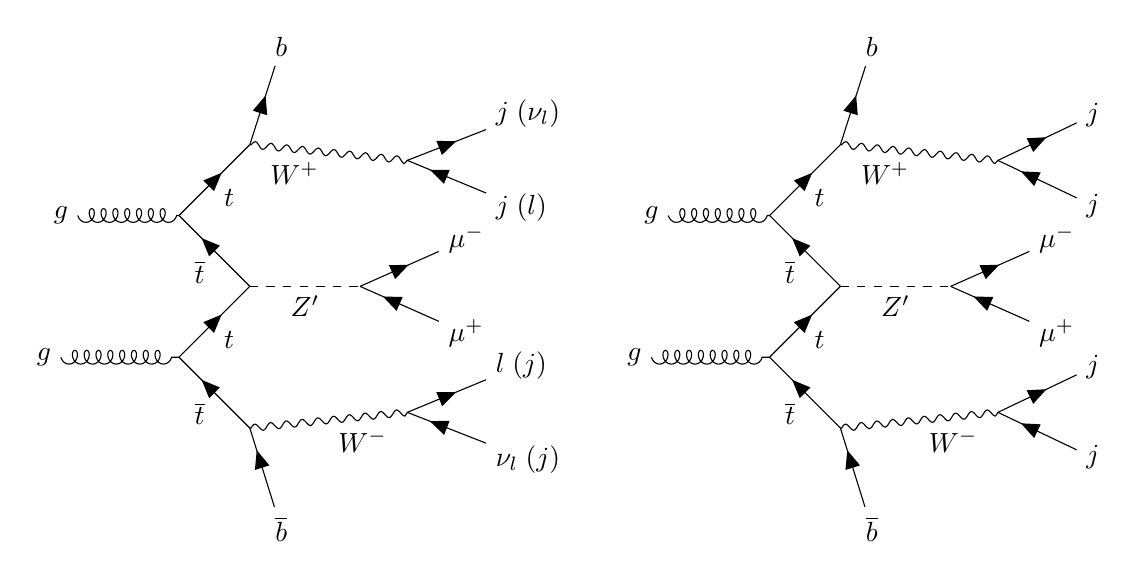
\begin{tikzpicture}
  \begin{feynman}
    \vertex (i1) {\(g\)};
    \vertex [right=of i1] (n11);
    \vertex [below right=0.9cm and 0.9cm of n11] (n22);
    \vertex [below left=0.9cm and 0.9cm of n22] (n12);
    \vertex [left=of n12] (i2) {\(g\)};
    
    \vertex [above right=0.9cm and 0.9cm of n11] (n21);
    \vertex [above right=1cm and 0.2cm of n21] (f1) {\(b\)};
    \vertex [below right=0.2cm and 2cm of n21] (n31);
    \vertex [above right=0.3cm and 1cm of n31] (f2) {\(j \; (\nu_l)\)};
    \vertex [below right=0.3cm and 1cm of n31] (f3) {\(j \; (l)\)};
    
    \vertex [below right=0.9cm and 0.9cm of n12] (n23);
    \vertex [below right=1cm and 0.2cm of n23] (f8) {\(\overline b\)};
    \vertex [above right=0.2cm and 2cm of n23] (n33);
    \vertex [above right=0.3cm and 1cm of n33] (f6) {\(l \; (j)\)};
    \vertex [below right=0.3cm and 1cm of n33] (f7) {\(\nu_{l} \; (j)\)};
    
    \vertex [right=1.4cm of n22] (n32);
    \vertex [above right=0.3cm and 1cm of n32] (f4) {\(\mu^{-}\)};
    \vertex [below right=0.3cm and 1cm of n32] (f5) {\(\mu^{+}\)};
    
    %SEGUNDO DIAGRAMA
    \vertex [right=7.5cm of i1] (j1) {\(g\)};
    \vertex [right=of j1] (m11);
    \vertex [below right=0.9cm and 0.9cm of m11] (m22);
    \vertex [below left=0.9cm and 0.9cm of m22] (m12);
    \vertex [left=of m12] (j2) {\(g\)};
    
    \vertex [above right=0.9cm and 0.9cm of m11] (m21);
    \vertex [above right=1cm and 0.2cm of m21] (g1) {\(b\)};
    \vertex [below right=0.2cm and 2cm of m21] (m31);
    \vertex [above right=0.3cm and 1cm of m31] (g2) {\(j\)};
    \vertex [below right=0.3cm and 1cm of m31] (g3) {\(j\)};
    
    \vertex [below right=0.9cm and 0.9cm of m12] (m23);
    \vertex [below right=1cm and 0.2cm of m23] (g8) {\(\overline b\)};
    \vertex [above right=0.2cm and 2cm of m23] (m33);
    \vertex [above right=0.3cm and 1cm of m33] (g6) {\(j\)};
    \vertex [below right=0.3cm and 1cm of m33] (g7) {\(j\)};
    
    \vertex [right=1.4cm of m22] (m32);
    \vertex [above right=0.3cm and 1cm of m32] (g4) {\(\mu^{-}\)};
    \vertex [below right=0.3cm and 1cm of m32] (g5) {\(\mu^{+}\)};

    \diagram* {
      (i1) -- [gluon] (n11) -- [anti fermion, edge label'=\(\overline t\)] (n22),
      (i2) -- [gluon] (n12) -- [fermion, edge label'=\(t\)] (n22),
      
      (n11) -- [fermion, edge label'=\(t\)] (n21) -- [boson, edge label'=\(W^{+}\)] (n31),
      (n31) -- [fermion] (f2), (n31) -- [anti fermion] (f3),
      (n21) -- [fermion] (f1),
      
      (n12) -- [anti fermion, edge label'=\(\overline t\)] (n23) -- [boson, edge label'=\(W^{-}\)] (n33),
      (n33) -- [fermion] (f6), (n33) -- [anti fermion] (f7),
      (n23) -- [anti fermion] (f8),
      
      (n22) -- [scalar, edge label'=\(Z'\)] (n32),
      (n32) -- [fermion] (f4), (n32) -- [anti fermion] (f5),
      
      %SEGUNDO DIAGRAMA
      (j1) -- [gluon] (m11) -- [anti fermion, edge label'=\(\overline t\)] (m22),
      (j2) -- [gluon] (m12) -- [fermion, edge label'=\(t\)] (m22),
      
      (m11) -- [fermion, edge label'=\(t\)] (m21) -- [boson, edge label'=\(W^{+}\)] (m31),
      (m31) -- [fermion] (g2), (m31) -- [anti fermion] (g3),
      (m21) -- [fermion] (g1),
      
      (m12) -- [anti fermion, edge label'=\(\overline t\)] (m23) -- [boson, edge label'=\(W^{-}\)] (m33),
      (m33) -- [fermion] (g6), (m33) -- [anti fermion] (g7),
      (m23) -- [anti fermion] (g8),
      
      (m22) -- [scalar, edge label'=\(Z'\)] (m32),
      (m32) -- [fermion] (g4), (m32) -- [anti fermion] (g5),
    };
  \end{feynman}
\end{tikzpicture}
\]
\vspace{-1\baselineskip}
\caption{Feynman diagrams of the two different channels of production and decay of $Z^{\prime}$ to be studied in the thesis, being these the semi-leptonic and fully-hadronic channels respectively.}
\label{diagrams}
\end{figure}

\subsection{Preliminary analysis} \label{ssec:1prelimresult}

\subsubsection{Leading order leptons}

The leading order leptons are the leptons generated with the highest transverse momentum, $\bm{p}_T$, and are denoted with a subindex 1. Normally, in the presence of other muons than the ones generated by the $Z^{\prime}$, it is expected that almost all leptons of leading order are the muons produced from the $Z^{\prime}$, due to its high mass, although in the fully-hadronic channel, no other final state leptons are generated. From relativity we know $E^2 = m^2 + \bm{p}^2$ (setting $c=1$), where in the case of the $Z^{\prime}: m(Z^{\prime}) \gg |\bm{p}(Z^{\prime})|$, and so $E(Z^{\prime}) \approx m(Z^{\prime})$, and for the muons: $m(\mu) \ll |\bm{p}(\mu)|$ due to the small mass of the muons, so $E(\mu) \approx |\bm{p}(\mu)|$. Because $m(Z^{\prime})\gg|\bm{p}(Z^{\prime})|$, most of its momentum is still on the $z$-axis, such that $\bm{p}_{T}(Z^{\prime})\approx 0$, then because of four-momentum conservation at the vertices of the interaction: $\bm{p}(\mu) \approx \bm{p}_{T}(\mu)$ and the muons are produced such that $\bm{p}_{T}(\mu^+) \approx -\bm{p}_{T}(\mu^-)$, therefore $|\bm{p}_{T}(\mu)| \approx m(Z^{\prime})/2$.


\begin{figure}[ht!]
     \begin{center}
        \subfigure[Distribution of $|\bm{p}_T|$ for $\mu_1$.]{
            \label{PTmu}
            \includegraphics[width=0.45\textwidth]{Sections/images/Preliminary/PTmu.png}
        }
        \subfigure[Distribution of $\phi$ for $\mu_1$.]{%
           \label{PHImu}
           \includegraphics[width=0.45\textwidth]{Sections/images/Preliminary/PHImu.png}
        }\\
        \subfigure[Distribution of $\eta$ for $\mu_1$.]{
            \label{ETAmu}
            \includegraphics[width=0.45\textwidth]{Sections/images/Preliminary/ETAmu.png}
        }
        \subfigure[Distribution of $\Delta R$ for $\mu^+_1$ and $\mu^-_1$.]{
            \label{DRmu}
            \includegraphics[width=0.45\textwidth]{Sections/images/Preliminary/DRmu.png}
        }
    \end{center}
    \vspace{-1\baselineskip}
    \caption{ Kinematic distributions for a $Z^{\prime}$ boson mass of 1 TeV for $\textrm{a) }|\bm{p}_T|,\textrm{b) } \phi \textrm{ (the azimuth angle)},\textrm{c) } \eta$ and $\textrm{d) }\Delta R$, defined as in Equations (\ref{eqeta}) and (\ref{eqdR}) respectively, for the leading order muons, where the first three graphs are only for $\mu^+_1$, as $\mu^+_1$ and $\mu^-_1$ have a similar distributions for these variables.} 
   \label{preliminarygraphs1}
\end{figure}

As can be seen from Figure \ref{PTmu}, effectively, the peak of the distribution of transverse momentum is around $\bm{p}_{T}(\mu) \approx m(Z^{\prime})/2$, with the mean at 525.4 GeV, reconstructing the mass of the $Z^{\prime}$ used in the simulation. In Figure \ref{PHImu} it is observed that the production of $\mu^+$ and $\mu^-$ does not have a preferred direction in the transverse plane, which is expected as the cross section for these processes does not depend on $\phi$. To analyse Figures \ref{ETAmu} and \ref{DRmu}, is needed to recall the definitions of $\eta$ and $\Delta R$ given before (see Section \ref{ssec:variables}).

Figure \ref{ETAmu} confirms again the validity of the approximation $\bm{p}(\mu) \approx \bm{p}_{T}(\mu)$, as the mean of the distribution is in zero, with the peak also at zero, meaning in most of the events the muons are produced in the transverse plane, so that $\bm{p}_T \gg \bm{p}_z$ or $\bm{p}_z \approx 0$. Finally, Figure \ref{DRmu} shows that in the majority of cases, the $\mu^+, \mu^-$ pair is produced with a difference of $\Delta\phi=\pi$, which means that although they do not have a preferential production direction in the transverse plane, they are produced in opposite directions to ensure that $\bm{p}_T \approx 0$.

\subsubsection{Reconstructed masses}

\begin{figure}[ht!]
     \begin{center}
        \subfigure[Distribution of reconstructed mass $m_{Z^{\prime}}$.]{
            \label{Mzp}
            \includegraphics[width=0.45\textwidth]{Sections/images/Preliminary/Mzp.png}
        }
        \subfigure[Distribution of reconstructed mass $m_{t}$.]{%
           \label{Mt}
           \includegraphics[width=0.45\textwidth]{Sections/images/Preliminary/Mt.png}
        }
    \end{center}
    \vspace{-1\baselineskip}
    \caption{Distributions for a $Z^{\prime}$ boson mass of 1 TeV for the invariant mass using the two leading muons (a) and the reconstructed mass using the two leading jets and the bottom-quark (b).} 
   \label{preliminarymasses}
\end{figure}

In Figures \ref{Mzp} and \ref{Mt}, average values of around $\overline m_{Z^{\prime}} \approx 990.3 \textrm{ GeV}$ and a RMS value for $ m_t = 172.5 \textrm{ GeV}$ are obtained, according to the values of mass given to $Z^{\prime}$ for the events generated, and the actual accepted value of mass of the top quark $m_t = 172.9 \pm 0.4 \textrm{ GeV}$. Although, it is important to note that here there is certain ambiguity on the choice of particles with which the top is reconstructed, as this channel has a total of 4 $j$'s and 2 $b$'s. Therefore, there are six different ways in which we can assign the particles coming from the two tops if we order them by their $|\bm{p}_T|$. This problem will be further studied.

\subsubsection{Cross section}

In Figure \ref{cross}, interpolations of simulated data of the total cross section $\sigma$ vs mass of the $Z^{\prime}$ are plotted for different coupling constants $g_l$ and $g_h$, which are the couplings of the $Z^{\prime}$ to light and heavy fermions respectively. The $y$-axis is the logarithm of $\sigma$ in fb$^{-1}$. From this graph it can be observed that as expected, $\sigma \sim m^{-1}$, making heavier $Z^{\prime}$ bosons harder to detect, as the total cross section decreases, indicating that the probability that the $Z^{\prime}$ interact with particles of the SM, and in particular with $\mu^+$ and $\mu^-$, is smaller. Also as one would expect, from the $S$-matrix expansion, $\sigma$ is proportional to the coupling constants, so that making the interaction stronger increases the probability of these processes occurring.

\begin{figure}[ht]
    \centering
    \includegraphics[width=12cm]{Sections/images/Preliminary/cross.png}
    \caption{Linearized cross section $\ln(\sigma)$ as a function of $m(Z^{\prime})$.}
    \label{cross}
\end{figure}

After doing some studies of the different backgrounds mentioned before, it was determined that, at MadGraph level, the relevant backgrounds are the $t\overline t$ backgrounds, being the diboson and triboson processes very sub-dominant. Some preliminary results of different variables for the signal and these two different backgrounds, $t\overline th$ and $t\overline t/h$, for the fully hadronic decay process will be shown. Prior to doing that, a quick explanation of the backgrounds is given.

\subsubsection{First background: $t\overline t/h$} \label{ssec:firstbkg}

The first and most important background considered in the analysis has a similar structure to the signals, but instead of being mediated by a $Z^{\prime}$ boson, is mediated by SM mediators, excluding the presence of the higgs boson. This means that in such case, the $t\overline t$ pair annihilates producing a $Z$ boson, or an off-shell photon ($\gamma^*$), which then decay into the muon pair. The diagram of this background is shown in Figure \ref{bkg1}.

\begin{figure}[ht!]
\[
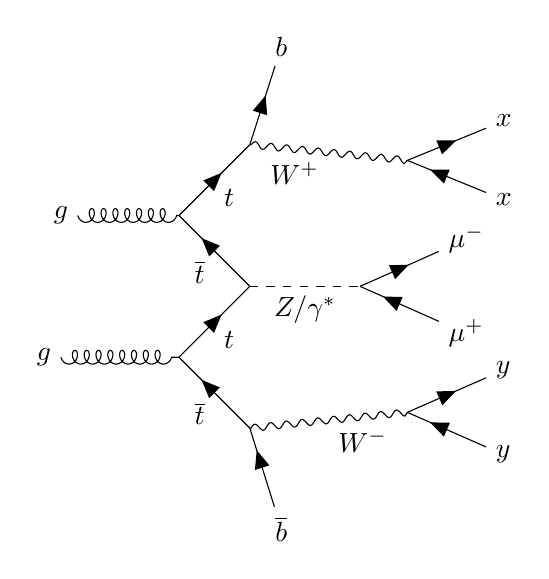
\begin{tikzpicture}
  \begin{feynman}
    \vertex (i1) {\(g\)};
    \vertex [right=of i1] (n11);
    \vertex [below right=0.9cm and 0.9cm of n11] (n22);
    \vertex [below left=0.9cm and 0.9cm of n22] (n12);
    \vertex [left=of n12] (i2) {\(g\)};
    
    \vertex [above right=0.9cm and 0.9cm of n11] (n21);
    \vertex [above right=1cm and 0.2cm of n21] (f1) {\(b\)};
    \vertex [below right=0.2cm and 2cm of n21] (n31);
    \vertex [above right=0.3cm and 1cm of n31] (f2) {\(x\)};
    \vertex [below right=0.3cm and 1cm of n31] (f3) {\(x\)};
    
    \vertex [below right=0.9cm and 0.9cm of n12] (n23);
    \vertex [below right=1cm and 0.2cm of n23] (f8) {\(\overline b\)};
    \vertex [above right=0.2cm and 2cm of n23] (n33);
    \vertex [above right=0.3cm and 1cm of n33] (f6) {\(y\)};
    \vertex [below right=0.3cm and 1cm of n33] (f7) {\(y\)};
    
    \vertex [right=1.4cm of n22] (n32);
    \vertex [above right=0.3cm and 1cm of n32] (f4) {\(\mu^{-}\)};
    \vertex [below right=0.3cm and 1cm of n32] (f5) {\(\mu^{+}\)};
    

    \diagram* {
      (i1) -- [gluon] (n11) -- [anti fermion, edge label'=\(\overline t\)] (n22),
      (i2) -- [gluon] (n12) -- [fermion, edge label'=\(t\)] (n22),
      
      (n11) -- [fermion, edge label'=\(t\)] (n21) -- [boson, edge label'=\(W^{+}\)] (n31),
      (n31) -- [fermion] (f2), (n31) -- [anti fermion] (f3),
      (n21) -- [fermion] (f1),
      
      (n12) -- [anti fermion, edge label'=\(\overline t\)] (n23) -- [boson, edge label'=\(W^{-}\)] (n33),
      (n33) -- [fermion] (f6), (n33) -- [anti fermion] (f7),
      (n23) -- [anti fermion] (f8),
      
      (n22) -- [scalar, edge label'=\(Z/\gamma^*\)] (n32),
      (n32) -- [fermion] (f4), (n32) -- [anti fermion] (f5),
    };
  \end{feynman}
\end{tikzpicture}
\]
\vspace{-1\baselineskip}
\caption{Feynman diagram of the first background, which excludes the production of a higgs boson ($h$).}
\label{bkg1}
\end{figure}

Here the $x$ and $y$ pairs can either be a pair of jets or a lepton-neutrino pair, depending on the signal being considered. In this background, the decay of the $Z$ into a pair of muons has a branching fraction of $(3.3662 \pm 0.0066)\%$.

To obtain this background, the following syntax was used in mg5 for the semi-leptonic channel:
\begin{alignat*}{2}
    &\texttt{mg5: generate p p $>$ t t$\sim$ mu+ mu- /h, (t > b j j), (t$\sim$ > b$\sim$ vl l) } \\
    &\texttt{mg5: add process p p $>$ t t$\sim$ mu+ mu- /h, (t > b vl l), (t$\sim$ > b$\sim$ j j)}
\end{alignat*}
in which /h is used to exclude the production of the higgs. For the fully-hadronic channel:
\begin{alignat*}{2}
    &\texttt{mg5: generate p p $>$ t t$\sim$ mu+ mu- /h, (t > b j j), (t$\sim$ > b$\sim$ j j) } \\
    &\texttt{mg5: add process p p $>$ t t$\sim$ mu+ mu- /h, (t > b j j), (t$\sim$ > b$\sim$ j j)}
\end{alignat*}

\subsubsection{Second background: $t\overline tWW$} \label{ssec:secondbkg}

This background is similar to the third one (Section \ref{ssec:thirdbkg}), but with an extra sub-process. The reason for this is that out of $5\times10^6$ simulated events for the semi-leptonic channel, and $10^6$ for the fully-hadronic, there was not a single event in which the higgs decayed into a pair of muons. In order to get around this problem, an intermediate decay of the higgs into $W$ bosons was included, with a branching fraction of $21.7\%$, which then decay leptonically, with a branching fraction of $10.63 \pm 0.15\%$, producing the two final state muons necessary for the event to be considered as a background of the signal. In this case, just as with the previous background, the pair of particles $x$ and $y$ may be either a pair of jets, or a pair of lepton-neutrino. The Feynman diagram of such process is shown below:

\begin{figure}[ht!]
\[
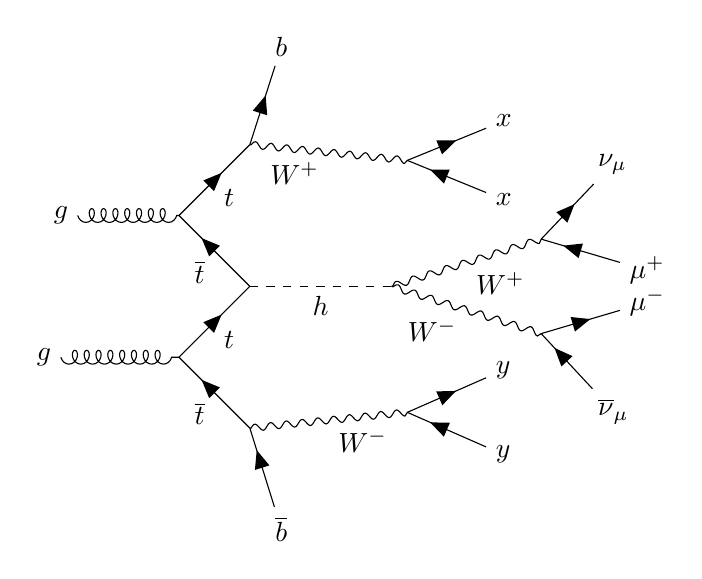
\begin{tikzpicture}
  \begin{feynman}
    \vertex (i1) {\(g\)};
    \vertex [right=of i1] (n11);
    \vertex [below right=0.9cm and 0.9cm of n11] (n22);
    \vertex [below left=0.9cm and 0.9cm of n22] (n12);
    \vertex [left=of n12] (i2) {\(g\)};
    
    \vertex [above right=0.9cm and 0.9cm of n11] (n21);
    \vertex [above right=1cm and 0.2cm of n21] (f1) {\(b\)};
    \vertex [below right=0.2cm and 2cm of n21] (n31);
    \vertex [above right=0.3cm and 1cm of n31] (f2) {\(x\)};
    \vertex [below right=0.3cm and 1cm of n31] (f3) {\(x\)};
    
    \vertex [below right=0.9cm and 0.9cm of n12] (n23);
    \vertex [below right=1cm and 0.2cm of n23] (f8) {\(\overline b\)};
    \vertex [above right=0.2cm and 2cm of n23] (n33);
    \vertex [above right=0.3cm and 1cm of n33] (f6) {\(y\)};
    \vertex [below right=0.3cm and 1cm of n33] (f7) {\(y\)};
    
    \vertex [right=1.8cm of n22] (n32);
    \vertex [above right=0.6cm and 1.9cm of n32] (n41);
    \vertex [below right=0.6cm and 1.9cm of n32] (n42);
    
    \vertex [above right=0.7cm and 0.6cm of n41] (f4) {\(\nu_{\mu}\)};
    \vertex [below right=0.1cm and 1cm of n41] (f5) {\(\mu^+\)};
    \vertex [above right=0.1cm and 1cm of n42] (f9) {\(\mu^-\)};
    \vertex [below right=0.7cm and 0.6cm of n42] (f10) {\(\overline \nu_{\mu}\)};
    
        \diagram* {
      (i1) -- [gluon] (n11) -- [anti fermion, edge label'=\(\overline t\)] (n22),
      (i2) -- [gluon] (n12) -- [fermion, edge label'=\(t\)] (n22),
      
      (n11) -- [fermion, edge label'=\(t\)] (n21) -- [boson, edge label'=\(W^{+}\)] (n31),
      (n31) -- [fermion] (f2), (n31) -- [anti fermion] (f3),
      (n21) -- [fermion] (f1),
      
      (n12) -- [anti fermion, edge label'=\(\overline t\)] (n23) -- [boson, edge label'=\(W^{-}\)] (n33),
      (n33) -- [fermion] (f6), (n33) -- [anti fermion] (f7),
      (n23) -- [anti fermion] (f8),
      
      (n22) -- [scalar, edge label'=\(h\)] (n32),
      (n32) -- [boson, edge label'=\(W^{+}\)] (n41),
      (n32) -- [boson, edge label'=\(W^{-}\)] (n42),
      
      (n41) -- [fermion] (f4), (n41) -- [anti fermion] (f5),
      (n42) -- [fermion] (f9), (n42) -- [anti fermion] (f10),
    };
  \end{feynman}
\end{tikzpicture}
\]
\vspace{-1\baselineskip}
\caption{\label{diagramas} Feynman diagram of the second background, which includes the production of a higgs boson, indirectly decaying to a muon pair.}
\label{bkg2}
\end{figure}

To generate this background, the results obtained for a similar process to that of Figure \ref{bkg3}, but generating $\tau$'s instead of $\mu$'s were used. This is because unlike muons, the coupling of the higgs to taus is considerably bigger due to its higher mass, having a branching fraction of around $6.24\%$. Then, this process's cross section was re-scaled such that
\begin{equation*}
    \sigma = \sigma_{\tau} \times \dfrac{B_{h \rightarrow W, W}}{B_{h \rightarrow \tau, \tau}} \times (B_{W \rightarrow \mu, \nu_{\mu}})^2 = 4.3623 \times \dfrac{0.217}{0.0624} \times (0.1063)^2 \textrm{ fb}^{-1} \approx 0.1714 \textrm{ fb}^{-1},
\end{equation*}
where $\sigma$ is the new cross section for this background, $\sigma_{\tau}$ is the cross section of the event corresponding to the Feynman diagram in Figure \ref{bkg3}, but replacing the muons coming from the $t\overline t$ annihilation by taus, and $B_p$ is the branching fraction of the process $p$. For example, 21.7\% of times that the higgs decays, it decays into a pair of $W^{\pm}$ bosons, such that $B_{h \rightarrow W, W} = 0.217$. The squared in $B_{W \rightarrow \mu, \nu_{\mu}}$ is due to the fact that both $W$'s have to decay into second generation leptons, having both processes the same branching fraction. The syntax used in mg5 to generate the process associated to $\sigma_{\tau}$ for the semi-leptonic and fully-hadronic channels was the same as for the third background.

\subsubsection{Third background: $t\overline th$} \label{ssec:thirdbkg}

The third background is also mediated by the production of a higgs bosons, which decays directly into muons. Nevertheless, as mentioned before, and due to the comparatively low mass of muons with respect to that of taus, the coupling of muons to the higgs bosons, mediated by their mass, is very small. Because of this, out of $5\times10^6$ events for the semi-leptonic channel, and $10^6$ for the fully-hadronic, not once did the higgs decay to muons: it always decayed into taus, as the mass of the electron is around 207 times smaller than that of the muon, being its expected coupling to higgs even smaller than that of muons. Therefore, this background is naturally suppressed, as it does not produce the two final state muons required. To generate this background, the following syntax was used in mg5 for the semi-leptonic channel:
\begin{alignat*}{2}
    &\texttt{mg5: generate p p $>$ t t$\sim$ h, (h > l+ l-), (t > b j j), (t$\sim$ > b$\sim$ vl l)} \\
    &\texttt{mg5: add process p p $>$ t t$\sim$ h, (h > l+ l-), (t > b vl l), (t$\sim$ > b$\sim$ j j)}
\end{alignat*}
and for the fully-hadronic channel:
\begin{alignat*}{2}
    &\texttt{mg5: generate p p $>$ t t$\sim$ h, (h > l+ l-), (t > b j j), (t$\sim$ > b$\sim$ j j)} \\
    &\texttt{mg5: add process p p $>$ t t$\sim$ h, (h > l+ l-), (t > b j j), (t$\sim$ > b$\sim$ j j)}
\end{alignat*}
where \texttt{l-} (\texttt{l+}) is a multiparticle defined such that in contains the three (anti)-leptons $e^-, \mu^-, \tau^-$ ($e^+, \mu^+, \tau^+$).

The Feynman diagram of this process is shown below, where again, the pair of particles $x$ and $y$ can either be a pair of jets or lepton-neutrino.

\begin{figure}[ht!]
\[
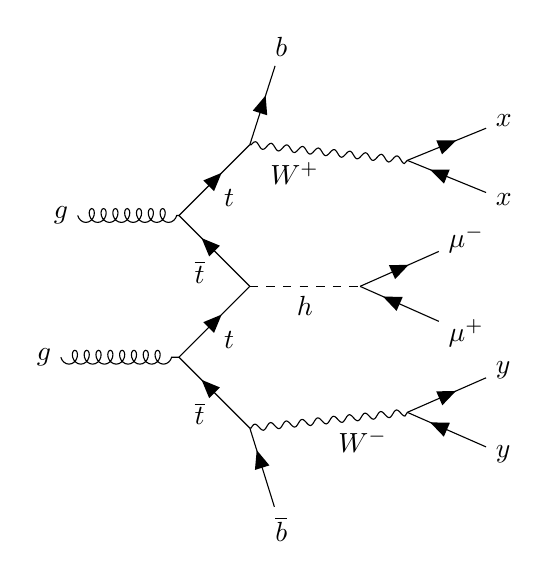
\begin{tikzpicture}
  \begin{feynman}
    \vertex (i1) {\(g\)};
    \vertex [right=of i1] (n11);
    \vertex [below right=0.9cm and 0.9cm of n11] (n22);
    \vertex [below left=0.9cm and 0.9cm of n22] (n12);
    \vertex [left=of n12] (i2) {\(g\)};
    
    \vertex [above right=0.9cm and 0.9cm of n11] (n21);
    \vertex [above right=1cm and 0.2cm of n21] (f1) {\(b\)};
    \vertex [below right=0.2cm and 2cm of n21] (n31);
    \vertex [above right=0.3cm and 1cm of n31] (f2) {\(x\)};
    \vertex [below right=0.3cm and 1cm of n31] (f3) {\(x\)};
    
    \vertex [below right=0.9cm and 0.9cm of n12] (n23);
    \vertex [below right=1cm and 0.2cm of n23] (f8) {\(\overline b\)};
    \vertex [above right=0.2cm and 2cm of n23] (n33);
    \vertex [above right=0.3cm and 1cm of n33] (f6) {\(y\)};
    \vertex [below right=0.3cm and 1cm of n33] (f7) {\(y\)};
    
    \vertex [right=1.4cm of n22] (n32);
    \vertex [above right=0.3cm and 1cm of n32] (f4) {\(\mu^{-}\)};
    \vertex [below right=0.3cm and 1cm of n32] (f5) {\(\mu^{+}\)};
    

    \diagram* {
      (i1) -- [gluon] (n11) -- [anti fermion, edge label'=\(\overline t\)] (n22),
      (i2) -- [gluon] (n12) -- [fermion, edge label'=\(t\)] (n22),
      
      (n11) -- [fermion, edge label'=\(t\)] (n21) -- [boson, edge label'=\(W^{+}\)] (n31),
      (n31) -- [fermion] (f2), (n31) -- [anti fermion] (f3),
      (n21) -- [fermion] (f1),
      
      (n12) -- [anti fermion, edge label'=\(\overline t\)] (n23) -- [boson, edge label'=\(W^{-}\)] (n33),
      (n33) -- [fermion] (f6), (n33) -- [anti fermion] (f7),
      (n23) -- [anti fermion] (f8),
      
      (n22) -- [scalar, edge label'=\(h\)] (n32),
      (n32) -- [fermion] (f4), (n32) -- [anti fermion] (f5),
    };
  \end{feynman}
\end{tikzpicture}
\]
\vspace{-1\baselineskip}
\caption{Feynman diagram of the third background, associated with the production of a higgs boson ($h$).}
\label{bkg3}
\end{figure}

\subsubsection{Top quark mass reconstruction}

Since in the fully hadronic process, as mentioned before, two pairs of jets are produced together with two  $b$-quarks, it is necessary to accurately determine which $j$'s and $b$'s came from the same mother particles, without relying on asking MadAnalysis if the mother particle of two given particles is the same, as this cannot be done experimentally. To do this, we analyse the different possible pairs of particles and see which ones are those that reconstruct best the mass of the top quark. 

For this first part of the analysis, it was found that the pairs of particles that seem to better reconstruct the mass of the top were $(j_1,j_4,b_2)$ and $(j_2,j_3,b_1)$. Here the sub-index as always denotes the order of particles from highest to lowest $\bm{p}_T$. For these pairs of particles, the histograms obtained of reconstructed mass for the top are shown in Figure \ref{Mtbien}.

\begin{figure}[ht!]
     \begin{center}
        \subfigure[Distribution of $m(t)$]{
            \label{Mtbien1}
            \includegraphics[width=0.45\textwidth]{Sections/images/Signal/Mtbien1.png}
        }
        \subfigure[Distribution of $m(t)$]{%
           \label{Mtbien2}
           \includegraphics[width=0.45\textwidth]{Sections/images/Signal/Mtbien2.png}
        }
    \end{center}
    \caption{Distribution of reconstructed mass, $m_(t)$, of the top quark for: a) the pair $(j_1, j_4, b_2)$ and b) the pair $(j_2, j_3, b_1)$.} 
    \label{Mtbien}
\end{figure}

For the other five different possible pairs, distributions with heavy tails or with peaks in wrong values of $m(t)$ were obtained, some of these are presented in Figure \ref{Mtmal} and show that in the majority of cases, these pairs did not correctly reconstruct the top. This is reflected on the value of the peak, which is significantly smaller compared to the ones shown in Figures \ref{Mtbien1} and \ref{Mtbien2}.

\begin{figure}[ht!]
     \begin{center}
        \subfigure[$m(t)$ distribution for the pair $(j_1,j_2,b_1)$.]{
            \label{Mtmal1}
            \includegraphics[width=0.45\textwidth]{Sections/images/Signal/Mtmal1.png}
        }
        \subfigure[$m(t)$ distribution for the pair $(j_1,j_2,b_2)$.]{
            \label{Mtmal2}
            \includegraphics[width=0.45\textwidth]{Sections/images/Signal/Mtmal2.png}
        }\\
        \subfigure[$m(t)$ distribution for the pair $(j_3,j_4,b_1)$.]{
            \label{Mtmal3}
            \includegraphics[width=0.45\textwidth]{Sections/images/Signal/Mtmal3.png}
        }
        \subfigure[$m(t)$ distribution for the pair $(j_3,j_4,b_2)$.]{
            \label{Mtmal4}
            \includegraphics[width=0.45\textwidth]{Sections/images/Signal/Mtmal4.png}
        }
    \end{center}
    \caption{Distribution of reconstructed $m(t)$ mass of the top quark for other possible pairs of jets and b-quark different from those of Figure \ref{Mtbien}.} 
    \label{Mtmal}
\end{figure}

As can be seen for example in Figures \ref{Mtmal2} or \ref{Mtmal3}, it seems that the pairs of jets (1,2) and (3,4) can also reconstruct correctly (with not so heavy tails) the mass of the $t$. Nevertheless, the pairs (1,4) and (2,3) shown in Figure \ref{Mtbien} not only have smaller tails, but as will be noted in the next section, pairs (1,2) and (3,4) do not reconstruct $m_W$ as correctly as the pairs (1,4) and (2,3).

\subsubsection{$W$ boson mass construction}

To further check if the top pairs did decay the majority of times in the pairs $(j_1,j_4,b_2)$ and $(j_2,j_3,b_1)$, the reconstructed mass of the $W^{\pm}$ was also checked. As mentioned before, even though the pairs $(j_1, j_2)$ and $(j_3, j_4)$ seemed to also be related one another via mass reconstruction of the top, it can be seen that for the mass of the $W^{\pm}$ bosons, these pairs present heavier tails (these graphs are shown in Figure \ref{MWbien1} through \ref{MWmal2}):

\begin{figure}[ht!]
     \begin{center}
        \subfigure[$m(W)$ distribution for the pair $(j_1, j_4)$.]{
            \label{MWbien1}
            \includegraphics[width=0.45\textwidth]{Sections/images/Signal/MWbien1.png}
        }
        \subfigure[$m(W)$ distribution for the pair $(j_2, j_3)$.]{
            \label{MWbien2}
            \includegraphics[width=0.45\textwidth]{Sections/images/Signal/MWbien2.png}
        }\\
        \subfigure[$m(W)$ distribution for the pair $(j_1, j_2)$.]{
            \label{MWmal1}
            \includegraphics[width=0.45\textwidth]{Sections/images/Signal/MWmal1.png}
        }
        \subfigure[$m(W)$ distribution for the pair $(j_3, j_4)$.]{
            \label{MWmal2}
            \includegraphics[width=0.45\textwidth]{Sections/images/Signal/MWmal2.png}
        }
    \end{center}
    \caption{Distribution of reconstructed mass $m_{W}$ of the $W^{\pm}$ bosons for different possible pairs of jets.} 
    \label{MWbienymal}
\end{figure}

Although it may be concluded that the pairs $(j_1, j_4, b_2)$ and $(j_2, j_3, b_1)$ reconstruct both top-quarks the majority of times, this will be further studied in the next section with madAnalysis expert mode. Additionally, the $\bm{p}_T$ of the two leading order muons, the ones coming from the $t\overline t$ annihilation, are shown in Figure \ref{Mmumal}.

From Figures \ref{Mmumal1} and \ref{Mmumal2}, it is observed that the higgs background ($t\overline th$) is suppressed, as out of this preliminary sample of $10^4$ events, no higgs boson decayed to muons. This is expected, as the decay width of the higgs decaying to muons is very small, since the higgs couples to particles by their mass, meaning that, the bigger the mass of the particles, the bigger the coupling constant, and therefore the branching fraction of this decay. Recent studies of this decay at the LHC have set an upper limit to this branching fraction of $6.4\times10^{-4}$ \cite{higgs1}, $4.7\times10^{-4}$ \cite{higgs2} and $0.8\times10^{-4} < B_{h \rightarrow \mu,\mu} < 4.5\times10^{-4}$ \cite{higgsmumu}.

\begin{figure}[ht!]
     \begin{center}
        \subfigure[Distribution of $\bm{p}_T(\mu_1)$]{
            \label{Mmumal1}
            \includegraphics[width=0.45\textwidth]{Sections/images/Signal/Mlep1.png}
        }
        \subfigure[Distribution of $\bm{p}_T(\mu_2)$]{%
           \label{Mmumal2}
           \includegraphics[width=0.45\textwidth]{Sections/images/Signal/Mlep2.png}
        }
    \end{center}
    \caption{Distribution of $\bm{p}_T$ of the two leading order muons.} 
    \label{Mmumal}
\end{figure}

\begin{comment}
\subsubsection{Signal over background histograms}

Finally, from this preliminary analysis, a series of histograms where the signal is bigger than the backgrounds were obtained. These histograms are very useful, as from them, one can determine the selection criteria necessary to separate signals from backgrounds.

\begin{figure}[ht!]
     \begin{center}
        \subfigure[$\bm{p}_T$ of $j_1$.]{
            \label{soverb1}
            \includegraphics[width=0.45\textwidth]{Sections/images/Signal/señal1.png}
        }
        \subfigure[$\Delta R$ between $j_1$ and $j_2$.]{
            \label{soverb2}
            \includegraphics[width=0.45\textwidth]{Sections/images/Signal/señal2.png}
        }\\
        \subfigure[$\bm{p}_T$ of $b_1$.]{
            \label{soverb3}
            \includegraphics[width=0.45\textwidth]{Sections/images/Signal/señal3.png}
        }
        \subfigure[$\Delta\bm{p}_T$ between $b_1$ and $b_2$.]{
            \label{soverb4}
            \includegraphics[width=0.45\textwidth]{Sections/images/Signal/señal4.png}
        }
    \end{center}
    \caption{Histogram with higher signal over background results for different topological and kinematic variables.} 
    \label{soverb}
\end{figure}
\end{comment}

\subsection{MadAnalysis expert mode} \label{ssec:resultsexpertmode}

In the last section, a preliminary run of the fully-hadronic channel for 10000 events was presented. In this section, both channels will be further studied, that is: perform specific cuts to the events to further distinguish the signal over the backgrounds, try to correctly reconstruct and tag the final state particles, and also study the semi-leptonic channel. For this, MadAnalysis in expert mode (see Section \ref{ssec:expertmode}), together with samples for the semi-leptonic (fully-hadronic) channel of $5\times10^5$ ($10^6$) events for the signal, and $5\times10^6$ ($10^6$) events for the backgrounds were used.

\subsubsection{Semi-leptonic channel} \label{ssec:semi-leptonic channel}

From the simulation of the signal and backgrounds for the semi-leptonic channel generated with MadGraph, the cross sections of these events can be obtained. Two different studies were carried out regarding the semi-leptonic channel: one for low masses of the $Z^{\prime}$, with $m(Z^{\prime}) < 350$ GeV, and another for high masses $m(Z^{\prime}) \geq 350$ GeV. Table \ref{crosssections} shows the different cross sections ($\sigma$) obtained for different masses of $Z^{\prime}$, including both low and high masses, and for the relevant backgrounds in GeV:

\begin{table}[ht!]
\centering
\caption{Table of the cross sections ($\sigma$) of the different signals and backgrounds used in the semi-leptonic analysis.}
\label{crosssections}
\begin{tabular}{cc}
\hline
\hline
Process & $\sigma$ (fb)$^{-1}$ \\
\hline
$m_{Z^{\prime}} = 125$ & $0.3337$ \\
$m_{Z^{\prime}} = 150$ & $0.2823$ \\
$m_{Z^{\prime}} = 250$ & $0.1670$ \\
$m_{Z^{\prime}} = 300$ & $0.1333$ \\
$m_{Z^{\prime}} = 350$ & $0.1080$ \\
$m_{Z^{\prime}} = 1000$ & $0.0134$ \\
$m_{Z^{\prime}} = 1500$ & $0.0041$ \\
$m_{Z^{\prime}} = 2500$ & $5.569\times10^{-4}$ \\
$t\overline t/h$ & $5.2420$ \\
$t\overline tWW$ & $0.1714$ \\
\hline
\hline
\end{tabular}
\end{table}

These results tell us that as one would expect, it is much more probable for the backgrounds to occur than the signals. Because of this, several different selection criteria for the events need to be applied, trying to exploit the differences between the kinematic and topological variables for the backgrounds and the signals. This, in order to eliminate the largest possible amount of events coming from the different backgrounds, affecting the signals as little as possible, so that the signals stand out over the backgrounds. In particular, five preliminary cuts (Section \ref{ssec:selectioncriteria}) where applied to distinguish $t\overline t$ processes from other possible process taking place at the LHC. 

Since the event analysis is made at MadAnalysis level, without considering hadronization shower and detector effects generated using Pythia and Delphes, the final state particles are composed by: two $b$-quarks coming from the top decay, two jets coming from one of the $W^{\pm}$ bosons generated by one of the top decays, one neutrino and lepton coming from the other $W^{\pm}$ boson from the other top decay, and two muons, coming from the $Z^{\prime}$ decay. Since a fully-leptonic decay, in which both tops decay leptonically is not considered, there will always be one pair of jets. Depending on how the daughter particles from the top that decays hadronically (or both in the fully-hadronic case) are produced, the events are classified into three categories:
\begin{itemize}
    \item Not merged: this case is when the two jets coming from the $W^{\pm}$ are not close together. This is measured by the $\Delta R$ between them, in particular when $\Delta R (j, \; j) > 0.8$, meaning that they are produced separated, and it is possible to experimentally differentiate their trajectories.
    \item Partially merged: this is when the two jets are produced close enough ($\Delta R (j, \; j) < 0.8$), then experimentally one would see a single object due to the closeness of the jets, a fat-jet ($j_f$). In partially merged cases, when the fat-jet is reconstructed, the $b$-quark coming from the weak interaction of the top decay is produced separated from the fat-jet, this is $\Delta R (b, \; j_f) > 1.0$.
    \item Fully merged: in this case, all daughter particles from the top decay are produced close to one another, meaning that not only one can see a fat-jet composed of the two jets from the $W^{\pm}$ decay, but as $\Delta R(b, \; j_f) < 1.0$, this fat-jet will also include the $b$-quark.
\end{itemize}

\paragraph{Primary selection criteria}\label{ssec:selectioncriteria}

In both cases, for high and low masses of $Z^{\prime}$, a set of five preliminary selection criteria, or cuts, were applied to the different signals and the relevant backgrounds, in order to experimentally be able to differentiate these events we are interested in, apart from any other possible process, taking advantage from the similar topology $t\overline t$ processes have. In Tables \ref{cut1} through \ref{cut5} these first five cuts are shown.

For convenience, lets denote the final state particles of the semi-leptonic decay in the following way: $j_1, j_2$, the jets coming from one of the $W^{\pm}$ decays, ordered by $\bm{p}_T$, as they are the only jets produced from these events, $b_1, b_2$, the two $b$-quarks coming from the top decays, $l, \nu_l$, the first or second generation lepton and neutrino coming from the other $W^{\pm}$ decay, and $\mu_1, \mu_2$, the two muons coming from the $Z^{\prime}$: here we assume we have already somehow tagged both muons coming from the $Z^{\prime}$, as in the case where $W^{\pm} \rightarrow \mu, \nu_{\mu}$, it is necessary to differentiate the muons coming from the $t\overline t$ annihilation, from the one coming from the $W$. In the notation for the muons coming from the $Z^{\prime}$, the sub-index does not necessarily represent their $\bm{p}_T$ ordering, as when $l$ is a muon, it could in some cases have higher $\bm{p}_T$ than $\mu_1$ and/or $\mu_2$. This is not expected to happen many times as we are considering higher masses of $Z^{\prime}$ than that of the $W$.

\begin{table}[ht!]
\centering
\caption{Table of the first cut applied to the events to characterize their topology.}
\label{cut1}
\begin{tabular}{cc}
\hline
\hline
 Criteria & Selections \\
\hline
 $N(\ell)$ & $\geq 1$ \\
 $|\bm{p}_T(l)|$ & $> 35\textrm{ GeV}$ \\
 $|\eta(l)|$ & $< 2.4$  \\
\hline
\hline
\end{tabular}
\end{table}

This first cut, shown in Table \ref{cut1}, differentiates by whether we are considering the case in which the leptonic decaying $W^{\pm}$ decays into first or second generation. In case the $W^{\pm}$ decays into first (second) generation fermions, we check that there is at least one electron (muon), $l$ in our notation, with a transverse momentum greater than 35 GeV, and $\eta$ smaller than 2.4. This criteria is applied as the mass of the electron (muon) and neutrino generated by the leptonic decaying $W^{\pm}$ are much more smaller than that of the $W$: approximately one would expect the lepton is produced with an energy of at least around half the mass of the $W$, giving some extra space for the experimental uncertainty in the measurement of the momentum. The value of $\eta$ is established from the experimental constrains of the tracking and muon detection systems, which have an angular coverage up to $\eta = 2.5$ and 2.4 respectively, as explained in Section $\ref{sec:colliders}$.

\begin{table}[ht!]
\centering
\caption{Table of the second cut applied to the events to characterize their topology.}
\label{cut2}
\begin{tabular}{cc}
\hline
\hline
 Criteria & Selections \\
\hline
 $N(j)$ & $= 2$ \\
 $|\bm{p}_T(j_i)|$ & $> 30\textrm{ GeV}$ \\
 $|\eta(j_i)|$ & $< 5$  \\
\hline
\hline
\end{tabular}
\end{table}

This cut checks that there are two jets, $j_i$, with $i=\{1,2\}$, the ones from the hadronic decaying $W$, with a transverse momentum greater than 30 GeV and $\eta$ less than 5, for reasons similar to those of the first cut. Naturally, as both conditions have to be fulfilled, this cut implicitly requires for the existence of exactly two jets in the final state particles.

\begin{table}[ht!]
\centering
\caption{Table of the third cut applied to the events to characterize their topology.}
\label{cut3}
\begin{tabular}{cc}
\hline
\hline
 Criteria & Selections \\
\hline
 $N(b)$ & $= 2$ \\
 $|\bm{p}_T(b_i)|$ & $> 30\textrm{ GeV}$ \\
 $|\eta(b_i)|$ & $< 2.4$  \\
\hline
\hline
\end{tabular}
\end{table}

The third cut, similar to the second cut, checks that there are two $b$-quarks, $b_i$, with $i=\{1,2\}$, the ones coming from the top decay, such that they have a transverse momentum greater than 30 GeV and an $\eta$ smaller than 2.4. This criteria also implicitly requires for the existence of two $b$-quarks.

\begin{table}[ht!]
\centering
\caption{Table of the fourth cut applied to the events to characterize their topology.}
\label{cut4}
\begin{tabular}{cc}
\hline
\hline
 Criteria & Selections \\
\hline
 $\slashed{E}_T$ & $> 30\textrm{ GeV}$  \\
\hline
\hline
\end{tabular}
\end{table}

This cut checks that the event has a total missing transverse energy greater than 30 GeV. This value for the cut is given by the fact that, as was explained before, one would expect the neutrino produced from the leptonic decaying $W^{\pm}$ to carry at least around half of the energy associated to the mass of the $W$, in case the $W$ decays at rest. This value gives the measurement some extra room for the uncertainty in the measurement of the missing energy at the LHC, which is of $\pm$10 GeV, establishing a lower limit for the measured amount of missing transverse energy the event must have.  

\begin{table}[ht!]
\centering
\caption{Table of the fifth cut applied to the events to characterize their topology.}
\label{cut5}
\begin{tabular}{cc}
\hline
\hline
 Criteria & Selections \\
\hline
 $N(\mu)$ & $\geq 2$ \\
 $|\bm{p}_T(\mu_i)|$ & $> 30\textrm{ GeV}$ \\
 $|\eta(\mu_i)|$ & $< 2.4$  \\
 $Q(\mu_1)\times Q(\mu_2)$ & < 1.0 \\
\hline
\hline
\end{tabular}
\end{table}

This final cut verifies several things: for starters, it checks the existence of two muons. This cut also checks that the two muons tagged as the ones coming from the $t\overline t$ annihilation have a $|\bm{p}_T| > 30$ GeV, as they are expected to be generated with high energy, due to the high mass of the $t\overline t$ pair. This cut also takes into account the aforementioned coverage of the muon detection system of $\eta < 2.4$. Finally, it checks that the multiplication of the charges of the muons tagged as the ones coming from the $t\overline t$ annihilation is smaller than 1.0, as if they were correctly tagged, we know their charges should multiply to $-1$.

Now, since the type of processes being studied produces three final state leptons, in order to know if the $W$ decayed into first or second generation, we need to be able to tell apart the two muons coming from the $t\overline t$ annihilation, such that we can check whether the other final state lepton is an electron or a muon. In order to do this, primarily the following criteria was used to tag these two muons: a loop over all final state leptons searched for all possible pairs of muons, and chose the ones coming from the $t\overline t$ annihilation as the ones with the smallest difference in their $\bm{p}_T$. This is, the ones such that $\Delta p_T = |\bm{p}_{T\mu_1}| - |\bm{p}_{T\mu_2}|$ is the smallest. Here, $\Delta p_T$ is positive definite, as the code loops over the muons from higher to smaller $\bm{p}_T$. The reason for this, is that they would be expected to carry around more or less the same $\bm{p}_T$: $\bm{p}_{T}(\mu) \approx m(Z^{\prime})/2$, which would also be expected to be much more higher than that of the other muon (when $W^{\pm} \rightarrow \mu, \nu_{\mu}$) in the high $Z^{\prime}$ masses cases.

Additionally, in case the events were catalogued as partially or fully merged, some of the cuts changed slightly, since as mentioned before, experimentally one would not detect two, but one (fat-)jet coming from the $W$ decay and two $b$-quarks, or in the fully-merged case, even only one fat-jet and one $b$-quark, as the $b$-quark produced by the leptonic decaying $W$ would also be produced close enough as to only see one fat-jet emitted from the $W$ decay. Then, as expected, the cuts change for these cases such that:

\vspace{0.2cm}

$\textbf{Partially merged events:}$

\begin{table}[ht!]
\centering
\caption{Table of the second cut applied to partially merged events.}
\label{cut2partially}
\begin{tabular}{cc}
\hline
\hline
 Criteria & Selections \\
\hline
 $N(j)$ & $= 1$ \\
 $|\bm{p}_T(j_f)|$ & $> 30\textrm{ GeV}$ \\
 $|\eta(j_f)|$ & $< 5$  \\
\hline
\hline
\end{tabular}
\end{table}

Now the second cut only checks if the fat-jet coming from both jets meets the criteria from Table $\ref{cut2}$.

\vspace{0.2cm}

$\textbf{Fully merged events:}$

Cut 2: Exactly the same second cut as for the partially merged case (Table \ref{cut2partially}).

\begin{table}[ht!]
\centering
\caption{Table of the third cut applied to fully merged events.}
\label{cut3fully}
\begin{tabular}{cc}
\hline
\hline
 Criteria & Selections \\
\hline
 $N(b)$ & $= 1$ \\
 $|\bm{p}_T(b)|$ & $> 30\textrm{ GeV}$ \\
 $|\eta(b)|$ & $< 2.4$  \\
\hline
\hline
\end{tabular}
\end{table}

In this case, only one $b$-quark is considered, as experimentally the one coming from the leptonic decaying $W$ is not differentiable from the two jets. Then, the third criteria only asks if the $b$-quark not used in the fat-jet reconstruction meets the criteria in Table $\ref{cut3}$.
 
The code used for this first analysis of the signal and backgrounds can be found on the GitHub user FelipeDiaz98, under the repository ``ma5-v3'': \url{https://github.com/FelipeDiaz98/ma5-v3}. In this folder two files can be found, the .h and .cpp as explained in Section \ref{ssec:codeframework}.

\paragraph{Efficiency} \label{ssec:efficiency}

When we start applying the cuts to the events, we have to quantify how good are these cuts at ruling out the background events, while keeping those from the signals as unaltered as possible. For this reason, we introduce the efficiency of a cut, say for example the $i$-th cut, as:
\begin{gather}
\label{eqeff}
    \epsilon_i = \dfrac{N_i}{N_{i-1}} \pm \delta \epsilon_i, \\
\label{eqefferr}
    \textrm{where:} \quad \delta \epsilon_i = \epsilon_i \sqrt{\dfrac{1}{N_i} + \dfrac{1}{N_{i-1}}},
\end{gather}
where $\epsilon_i$ is the efficiency of the $i$-th cut, $N_i$ is the number of events that passed the $i$-th cut, and $N_{i-1}$ are the events that passed the $i-1$-th cut, where naturally $N_0$ is the initial number of events after applying any cut. Additionally, $\delta\epsilon_i$ is the error, which is estimated assuming $N_i$ and $N_{i-1}$ as independent numbers, which is a good approximation when one of the numbers is much higher than the other. Then, the cumulative efficiency after applying $n$ cuts is defined as
\begin{equation*}
    \epsilon_c = \prod_{i=1}^{n}\epsilon_i = \dfrac{N_n}{N_0},
\end{equation*}
then, it is desirable that the cuts have efficiencies tending to 1 for the signals, while for the backgrounds tending to 0. 

The expected number of events of a given process, either signal or background, is estimated as:
\begin{equation}
\label{eqnumberofevents}
    \mathcal{N}_i = \epsilon_i\times \sigma\times L,
\end{equation}
where $\sigma$ is the production cross section, $\epsilon_i$ the cumulative efficiency, and $L$ the luminosity. This way, it is not important if the amount of generated events are different, as the efficiency is taken into account. This is, only the relative amount of events that pass a certain cut are counted, while also giving it a probabilistic sense as to how many events are expected experimentally after a certain cut is applied, as the cross section is also included. The total number of expected backgrounds is estimated as:
\begin{equation}
\label{eqnumberofeventsbkg}
    \mathcal{N}_B = \sum_i \epsilon_i \times \sigma_i \times L = \sum_{\textrm{bkg}}\mathcal{N}_{\textrm{bkg}},
\end{equation}
where the sum over $i$ is made over the different backgrounds.

\paragraph{High $Z^{\prime}$ boson masses}\label{ssec:highmass}

In this case, masses of the $Z^{\prime}$ boson above 350 GeV are considered. In particular, for this study the following masses were used: $m(Z^{\prime}) = \{$350, 500, 1000, 1500, 2000, 2500, 3000, 3500, 4000$\}$ in GeV. For each of these masses, a total of $5\times10^{5}$ events were simulated, and as mentioned before, in order to have as much statistics from the backgrounds as possible, for each of them a total of $5\times10^6$ events were simulated. The first five preliminary cuts, the ones in Section \ref{ssec:selectioncriteria}, were applied to these signals. Some of the important results obtained for the different variables after applying these cuts are shown below.

\begin{figure}[ht]
    \centering
    \includegraphics[width=10cm]{Sections/images/5_cuts_hm/N_Merged.png}
    \caption{Fraction of events falling in the categories of not, partially, and fully merged, for two of the main backgrounds and four different $Z^{\prime}$ masses.}
    \label{5cutsHm_Merged}
\end{figure}

Figure \ref{5cutsHm_Merged} shows the amount of events that were cataloged as not, partially and fully merged, normalized to unity, including both channels: $W^{\pm}\rightarrow e, \nu_e$ and $W^{\pm}\rightarrow \mu, \nu_{\mu}$. From this graph it can be seen that the majority of cases, from around 75\% to around 92\% of the events for the different signals, fall in the not-merged category.
The amount of not merged cases diminishes proportional to $m(Z^{\prime})$, while the fully merged cases increase with the mass, keeping the amount of partially merged cases almost equal for all processes.

$\bm{W^{\pm} \rightarrow e, \nu_e:}$ First, we will focus on the results obtained for the case in which the leptonic decaying $W$ decays into first generation leptons. In the results reported, only four different signals are shown together with the different backgrounds. In this case, the signals shown are for $m(Z^{\prime}) = \{$350, 1000, 1500, 2500$\}$ in GeV. Additionally, the $t\overline th$ background was suppressed, as the higgs never decayed to muons.

Now that with these first five cuts the $t\overline t$ processes are separated from other possible processes, it is desired to further clear the signal, this is, to reduce the number of events coming from the backgrounds. In order to do this, in Figure \ref{5cutsHm_Results_e} some plots were made for the events that passed the first five cuts, in order to look for a variable that would allow for the definition of a sixth cut:

\begin{figure}[ht!]
     \begin{center}
        \subfigure[Scalar sum of $\bm{p}_T$ for $\mu_1$ and $\mu_2$.]{
            \label{5cutsHm_PTScalar_e}
            \includegraphics[width=0.45\textwidth]{Sections/images/5_cuts_hm/PT_Scalar_leptons_e.png}
        }
        \subfigure[Vector sum of $\bm{p}_T$ for $\mu_1$ and $\mu_2$.]{%
           \label{5cutsHm_PTVector_e}
           \includegraphics[width=0.45\textwidth]{Sections/images/5_cuts_hm/PT_Vector_leptons_e.png}
        }\\
        \subfigure[$ST_{MET}$.]{
            \label{5cutsHm_StMet_e}
            \includegraphics[width=0.45\textwidth]{Sections/images/5_cuts_hm/StMet_e.png}
        }
    \end{center}
    \vspace{-1\baselineskip}
    \caption{Plots made after applying the first five cuts for high $Z^{\prime}$ masses in the $W^{\pm}\rightarrow e, \nu_e$ channel: a) Scalar sum of $\bm{p}_T$ for the two muons coming from the $t\overline t$ annihilation, b) Vector sum of $\bm{p}_T$ for the two muons coming from the $t\overline{ t}$ annihilation, c) Total scalar sum of $\bm{p}_T$ for the final state particles.} 
   \label{5cutsHm_Results_e}
\end{figure}

Figures \ref{5cutsHm_PTScalar_e} and \ref{5cutsHm_PTVector_e}, show the scalar and vectorial sum of the $\bm{p}_T$ between the two muon candidates from the $Z^{\prime}$ boson, respectively. Figure \ref{5cutsHm_StMet_e} shows the $ST_{MET}$ distribution. Note that the scalar sum of the $\bm{p}_T$ between the two muons peak at around the nominal signal mass, as expected, and gives a good separation among the signals and the backgrounds, better than the separation observed in the $ST_{MET}$ distribution. This result suggest the possibility of a sixth cut in the scalar sum of the muons coming from the $t\overline t$ annihilation of around 150 GeV.

Then, with these results from the first five backgrounds, a new sixth cut, shown in Table \ref{cut6} was defined. The code used to generate these results can be found under the repository ``ma5-v4'': \url{https://github.com/FelipeDiaz98/ma5-v4}. 
\begin{table}[ht!]
\centering
\caption{Table of the sixth cut applied to the events to eliminate backgrounds.}
\label{cut6}
\begin{tabular}{cc}
\hline
\hline
 Criteria & Selections \\
\hline
 $|\bm{p}_T(\mu_1)| + |\bm{p}_T(\mu_2)|$ & $> 150$ GeV  \\
\hline
\hline
\end{tabular}
\end{table}

After applying the sixth cut, the different kinematic and topological distributions obtained for the events that passed all six cuts were plotted. In figure \ref{6cutsHm_Mleptons_e}, the distribution obtained for the reconstructed dimuon mass normalized to the expected number of events is shown. Note that the last bin going from 1200-3000 GeV is an overflow bin made due to the lack of statistics for the backgrounds, as the higher the dimuon mass, the lower the number of background events.

\begin{figure}[ht]
    \centering
    \includegraphics[width=10cm]{Sections/images/6_cuts_hm/M_leptons_e.png}
    \caption{Reconstructed mass of the two muons coming from the $t\overline t$ annihilation after applying six cuts for the $e$ channel.}
    \label{6cutsHm_Mleptons_e}
\end{figure}

From the results obtained in Figure \ref{6cutsHm_Mleptons_e}, a seventh cut can be proposed, due to the fact that the backgrounds have their peaks in a small values of mass, unlike the signals, as they are produced from SM mediators, which are much more lighter than the $Z^{\prime}$ masses considered. Furthermore, it is important to notice that, as can be seen in Figure \ref{6cutsHm_Mleptons_e}, the signals are ``buried into the backgrounds'', as these have way more number of events (notice the $y$-axis of the graph is in log scale), this is because this graph uses the number of events $\mathcal{N}$ rather than $N$. Since the production cross sections for the backgrounds are higher than for the signals, the expected number of background events is larger with respect to the signal. Also, even though the backgrounds were generated with 10 times more events in order to have enough statistics, that does not play a relevant factor to the difference in order of magnitudes of number of events, as only the efficiencies, rather than $N$, are taken into account.

From Figure \ref{6cutsHm_Mleptons_e}, a seventh cut was proposed in order to further decrease the events from the backgrounds. Table \ref{cut7} shows the criteria used for this new cut.

\begin{table}[ht!]
\centering
\caption{Table of the seventh cut applied to the events to eliminate backgrounds.}
\label{cut7}
\begin{tabular}{cc}
\hline
\hline
 Criteria & Selections \\
\hline
 $m(\mu_1, \mu_2)$ & $> 290$ GeV  \\
\hline
\hline
\end{tabular}
\end{table}

The code used for the analysis of the seventh cut can be found in the folder ``ma5-v5'' in the link: \url{https://github.com/FelipeDiaz98/ma5-v5}. First, the plot of number of events ($N$) that passed each of the seven cuts is shown in Figure \ref{7cutsHm_Eff_e}. This figure is normalize to unity for each of the different processes considered separately.

\begin{figure}[ht!]
    \centering
    \includegraphics[width=10cm]{Sections/images/7_cuts_hm/Efficiencies_e.png}
    \caption{Plot of the number of events ($N$) for 7 cuts, high $Z^{\prime}$ masses and $W^{\pm}\rightarrow e, \nu_e$ channel, normalized to unity.}
    \label{7cutsHm_Eff_e}
\end{figure}

As can be seen from Figure \ref{7cutsHm_Eff_e}, with this last cut it is possible to filter almost all of the background events. The table obtained for the efficiencies ($\epsilon_i$) of each of the seven cuts and cumulative efficiency ($\epsilon_c$), together with the table of number of events ($\mathcal{N}_i$) after each cut in the $W^{\pm} \rightarrow e, \nu_e$ channel are shown in Tables \ref{Table_Eff_e} and \ref{Table_Num_e}. Remember that in the case of efficiencies, we desire values closer to 1 for the signals, while for the backgrounds we want an efficiency closer to 0. In Table \ref{Table_Eff_e}, the efficiencies are multiplied by 100, such that we want them (in percentage) to tend to 100 for the signals, rather than 1.

\begin{table}[ht!]
\centering
\caption{Table of efficiencies ($\epsilon$) of the seven cuts applied to the events for the $W^{\pm} \rightarrow e, \nu_e$ channel for high $Z^{\prime}$ masses.}
\label{Table_Eff_e}
\resizebox{\textwidth}{!}{\begin{tabular}{c|ccccccc|c}
\hline
\hline
Process & $\epsilon_1 \; (\%)$ & $\epsilon_2 \; (\%)$  & $\epsilon_3 \; (\%)$  & $\epsilon_4 \; (\%)$  & $\epsilon_5 \; (\%)$  & $\epsilon_6 \; (\%)$  & $\epsilon_7 \; (\%)$ & $\epsilon_c \; (\%)$ \\
\hline
$t\overline tWW$ & 64.4 $\pm$ 0.1 & 54.1 $\pm$ 0.2 & 73.6 $\pm$ 0.3 & 73.2 $\pm$ 0.3 & 86.8 $\pm$ 0.4 & 52.2 $\pm$ 0.3 & 0 & 0 \\
$t\overline t/h$ & 62.2 $\pm$ 0.1 & 53.6 $\pm$ 0.2 & 73.7 $\pm$ 0.3 & 73.2 $\pm$ 0.3 & 65.5 $\pm$ 0.3 & 56.6 $\pm$ 0.4 & 0.62 $\pm$ 0.04 & 0.041 $\pm$ 0.003\\
$m(Z^{\prime}) = 350$ & 63.9 $\pm$ 0.1 & 55.7 $\pm$ 0.2 & 76.1 $\pm$ 0.3 & 75.2 $\pm$ 0.3 & 94.3 $\pm$ 0.4 & 98.7 $\pm$ 0.5 & 94.5 $\pm$ 0.4 & 17.91 $\pm$ 0.06\\
$m(Z^{\prime}) = 1000$ & 67.6 $\pm$ 0.1 & 59.6 $\pm$ 0.2 & 77.2 $\pm$ 0.3 & 77.7 $\pm$ 0.3 & 97.5 $\pm$ 0.4 & 100.0 $\pm$ 0.4 & 99.8 $\pm$ 0.4 & 23.53 $\pm$ 0.08\\
$m(Z^{\prime}) = 1500$ & 69.4 $\pm$ 0.2 & 61.4 $\pm$ 0.2 & 78.1 $\pm$ 0.4 & 78.3 $\pm$ 0.4 & 97.8 $\pm$ 0.5 & 100.0 $\pm$ 0.6 & 99.9 $\pm$ 0.6 & 25.5 $\pm$ 0.1\\
$m(Z^{\prime}) = 2500$ & 71.7 $\pm$ 0.2 & 63.0 $\pm$ 0.2 & 78.4 $\pm$ 0.4 & 79.3 $\pm$ 0.4 & 98.2 $\pm$ 0.5 & 100.0 $\pm$ 0.5 & 99.9 $\pm$ 0.5 & 27.6 $\pm$ 0.1\\
\hline
\hline
\end{tabular}}
\end{table}

\begin{table}[ht!]
\centering
\caption{Table of number of events ($\mathcal{N}$) of the seven cuts applied to the events for the $W^{\pm} \rightarrow e, \nu_e$ channel for high $Z^{\prime}$ masses.}
\label{Table_Num_e}
\resizebox{\textwidth}{!}{\begin{tabular}{c|cccccccc}
\hline
\hline
Process & $\mathcal{N}_0$ & $\mathcal{N}_1$  & $\mathcal{N}_2$  & $\mathcal{N}_3$  & $\mathcal{N}_4$  & $\mathcal{N}_5$  & $\mathcal{N}_6$ & $\mathcal{N}_7$ \\
\hline
$t\overline tWW$ & $2.57\times10^1$ & $1.66\times10^1$ & 8.97 & 6.60 & 4.83 & 4.19 & 2.19 & 0 \\
$t\overline t/h$ & $7.86\times10^2$ & $4.89\times10^{2}$ & $2.62\times10^{2}$ & $1.93\times10^{2}$ & $1.41\times10^{2}$ & $9.26\times10^{1}$ & $5.24\times10^{1}$ & $3.26\times10^{-1}$ \\
$m(Z^{\prime}) = 350$ & $1.62\times10^1$ & $1.03\times10^{1}$ & 5.76 & 4.38 & 3.30 & 3.11 & 3.07 & 2.90 \\
$m(Z^{\prime}) = 1000$ & 2.01 & 1.36 & $8.12\times10^{-1}$ & $6.27\times10^{-1}$ & $4.87\times10^{-1}$ & $4.75\times10^{-1}$ & $4.74\times10^{-1}$ & $4.74\times10^{-1}$ \\
$m(Z^{\prime}) = 1500$ & $6.11\times10^{-1}$ & $4.24\times10^{-1}$ & $2.60\times10^{-1}$ & $2.03\times10^{-1}$ & $1.59\times10^{-1}$ & $1.56\times10^{-1}$ & $1.56\times10^{-1}$ & $1.56\times10^{-1}$ \\
$m(Z^{\prime}) = 2500$ & $8.35\times10^{-2}$ & $5.99\times10^{-2}$ & $3.77\times10^{-2}$ & $2.96\times10^{-2}$ & $2.35\times10^{-2}$ & $2.30\times10^{-2}$ & $2.30\times10^{-2}$ & $2.30\times10^{-2}$ \\
\hline
\hline
\end{tabular}}
\end{table}

From Table \ref{Table_Eff_e}, it can be seen that the first five cuts have slightly smaller efficiencies for the backgrounds than for the signals, because these cuts are not meant to rule out background events, but to characterise $t\overline t$ processes. The only exception is for the fifth cut for the $t\overline t/h$ background, which is considerably smaller than the rest of efficiencies for this cut, meaning that this cut filters out more events for this background than for the rest of processes. For the sixth and seventh cut it is observed how, consequence of the significantly smaller number of events for the backgrounds observed in Figure \ref{7cutsHm_Eff_e}, the efficiencies of these cuts are smaller than that for the signals, specially for the seventh cut, which eliminates completely the third background, and leaves only 0.62\% of the events that passed the first six cuts for the second background. This is reflected on the last column of Table \ref{Table_Num_e} (the one labeled $\mathcal{N}_7$), where it can be seen that with all seven cuts, even though the backgrounds initially had several order of magnitudes more number of events than the signals, the number of events of the signals are comparable to those of the backgrounds, and in the case of the 350 and 1000 GeV signals, they are even greater.

Finally, for the study of the significance of the four signals considered, the analysis will be done at the end in Section \ref{ssec:statistical} for the different channels, this is, for the electron and muon channel, for both, high and low mass signals.

$\bm{W^{\pm} \rightarrow \mu, \nu_{\mu}:}$ For the case in which one of the $W$'s decays leptonically to second generation leptons, the following results were obtained after applying the five preliminary cuts.

\begin{figure}[ht!]
     \begin{center}
        \subfigure[Scalar sum of $\bm{p}_T$ for $\mu_1$ and $\mu_2$.]{
            \label{5cutsHm_PTScalar_mu}
            \includegraphics[width=0.45\textwidth]{Sections/images/5_cuts_hm/PT_Scalar_leptons_mu.png}
        }
        \subfigure[Vector sum of $\bm{p}_T$ for $\mu_1$ and $\mu_2$.]{%
           \label{5cutsHm_PTVector_mu}
           \includegraphics[width=0.45\textwidth]{Sections/images/5_cuts_hm/PT_Vector_leptons_mu.png}
        }\\
        \subfigure[$ST_{MET}$.]{
            \label{5cutsHm_StMet_mu}
            \includegraphics[width=0.45\textwidth]{Sections/images/5_cuts_hm/StMet_mu.png}
        }
    \end{center}
    \vspace{-1\baselineskip}
    \caption{Plots made for the results of 5 cuts, high $Z^{\prime}$ masses and $W^{\pm}\rightarrow \mu, \nu_{\mu}$ channel: a) Scalar sum of $\bm{p}_T$ for the two muons coming from the $t\overline{ t}$ annihilation, b) Vector sum of $\bm{p}_T$ for the two muons coming from the $t\overline{ t}$ annihilation, c) Total scalar sum of $\bm{p}_T$ for the final state particles.} 
   \label{5cutsHm_Results_mu}
\end{figure}

With these results several things can be noted. First, from Figure \ref{5cutsHm_PTScalar_mu} it can be seen that it does seem that the method for tagging the two muons coming from the $Z^{\prime}$ is not correctly identifying them, as it can be seen that the lower the mass of $Z^{\prime}$, there tends to be another peak in the distribution of $|\bm{p}_T|$ shifted towards $m_{W^{\pm}}$, which should not be there, as the distribution should peak around $m(Z^{\prime})$. This can also be checked in the $e$ channel, where there is no ambiguity on the tagging of the muons, where the left maximum is not observed. 

Furthermore, it can also be seen that, just as with the $e$ channel, assuming one can correctly tag the muons, Figures \ref{5cutsHm_PTScalar_mu} and \ref{5cutsHm_StMet_mu} seem to also suggest a sixth cut to further differentiate the signal from the backgrounds. Because of this, a sixth cut equal to that shown in Table \ref{cut6} was applied to the events of the $\mu$ channel. The code used to generate this part of the analysis is the same as for the $e$ channel, and can be found in the ``ma5-v4'' repository. Also, in this part of the analysis, the method to tag the muons coming from the $Z^{\prime}$ was changed to the pair of muons that maximized the scalar sum of the momentum, this is, the ones such that $p_t = |\bm{p}_{\mu_1}| + |\bm{p}_{\mu_2}|$ was the biggest.

Similar to the case of six cuts for the $e$ channel, the reconstructed dimuon mass, the two muons coming from the $t\overline t$ annihilation, is plotted in Figure \ref{6cutsHm_Mleptons_mu}, in order to obtain a seventh cut that could help ruling out more background events.

\begin{figure}[ht]
    \centering
    \includegraphics[width=10cm]{Sections/images/6_cuts_hm/M_leptons_mu.png}
    \caption{Reconstructed mass of the two muons coming from the $t\overline t$ annihilation after applying six cuts for the $\mu$ channel.}
    \label{6cutsHm_Mleptons_mu}
\end{figure}

With the distribution obtained in Figure \ref{6cutsHm_Mleptons_mu}, it can be seen that, just as for the $e$ channel, the majority of events for the backgrounds are obtained for lower dimuon mass values. Therefore, a seventh cut for the $\mu$ channel similar to that of Table \ref{cut7} is applied. The code used to generate the results including this seventh cut is found under the repository ``ma5-v5''.

\vspace{0.6cm}

For this channel, the result of number of events obtained after each cut are shown in Figure \ref{7cutsHm_Eff_mu}. As can be seen, the backgrounds are diminished significantly with the last two cuts, while maintaining the number of events for the signals almost unaltered.

\begin{figure}[ht!]
    \centering
    \includegraphics[width=10cm]{Sections/images/7_cuts_hm/Efficiencies_mu.png}
    \caption{Plot of the number of events ($N$) for 7 cuts, high $Z^{\prime}$ masses and $W^{\pm}\rightarrow \mu, \nu_{\mu}$ channel, normalized to unity.}
    \label{7cutsHm_Eff_mu}
\end{figure}

With the results shown in Figure \ref{7cutsHm_Eff_mu}, it is again possible to determine all the efficiencies for the different cuts, and with them, obtain the number of events ($\mathcal{N}$) after each cut. The following tables show these results. Note again that in Table \ref{Table_Eff_mu}, the efficiencies are multiplied by 100.

\begin{table}[ht!]
\centering
\caption{Table of efficiencies ($\epsilon$) of the seven cuts applied to the events for the $W^{\pm} \rightarrow \mu, \nu_{\mu}$ channel for high $Z^{\prime}$ masses.}
\label{Table_Eff_mu}
\resizebox{\textwidth}{!}{\begin{tabular}{c|ccccccc|c}
\hline
\hline
Process & $\epsilon_1 \; (\%)$ & $\epsilon_2 \; (\%)$  & $\epsilon_3 \; (\%)$  & $\epsilon_4 \; (\%)$  & $\epsilon_5 \; (\%)$  & $\epsilon_6 \; (\%)$  & $\epsilon_7 \; (\%)$ & $\epsilon_c \; (\%)$ \\
\hline
$t\overline tWW$ & 64.3 $\pm$ 0.1 & 54.2 $\pm$ 0.2 & 73.9 $\pm$ 0.3 & 73.5 $\pm$ 0.3 & 86.6 $\pm$ 0.4 & 52.2 $\pm$ 0.3 & 0 & 0 \\
$t\overline t/h$ & 97.9 $\pm$ 0.2 & 52.9 $\pm$ 0.1 & 74.7 $\pm$ 0.2 & 79.8 $\pm$ 0.3 & 57.0 $\pm$ 0.2 & 62.4 $\pm$ 0.3 & 9.7 $\pm$ 0.1 & 1.06 $\pm$ 0.01 \\
$m(Z^{\prime}) = 350$ & 99.9 $\pm$ 0.2 & 54.8 $\pm$ 0.1 & 76.9 $\pm$ 0.2 & 81.0 $\pm$ 0.3 & 82.8 $\pm$ 0.3 & 98.6 $\pm$ 0.4 & 92.0 $\pm$ 0.4 & 25.62 $\pm$ 0.08 \\
$m(Z^{\prime}) = 1000$ & 100.0 $\pm$ 0.2 & 58.8 $\pm$ 0.1 & 78.3 $\pm$ 0.2 & 82.5 $\pm$ 0.3 & 94.6 $\pm$ 0.3 & 100.0 $\pm$ 0.3 & 99.7 $\pm$ 0.3 & 35.8 $\pm$ 0.1 \\
$m(Z^{\prime}) = 1500$ & 100.0 $\pm$ 0.3 & 60.7 $\pm$ 0.2 & 78.7 $\pm$ 0.3 & 83.1 $\pm$ 0.4 & 96.7 $\pm$ 0.4 & 100.0 $\pm$ 0.5 & 100.0 $\pm$ 0.5 & 38.4 $\pm$ 0.1 \\
$m(Z^{\prime}) = 2500$ & 100.0 $\pm$ 0.3 & 62.4 $\pm$ 0.2 & 79.1 $\pm$ 0.3 & 83.5 $\pm$ 0.4 & 98.0 $\pm$ 0.4 & 100.0 $\pm$ 0.4 & 99.9 $\pm$ 0.4 & 40.3 $\pm$ 0.2 \\
\hline
\hline
\end{tabular}}
\end{table}

\begin{table}[ht!]
\centering
\caption{Table of number of events ($\mathcal{N}$) of the seven cuts applied to the events for the $W^{\pm} \rightarrow \mu, \nu_{\mu}$ channel for high $Z^{\prime}$ masses.}
\label{Table_Num_mu}
\resizebox{\textwidth}{!}{\begin{tabular}{c|cccccccc}
\hline
\hline
Process & $\mathcal{N}_0$ & $\mathcal{N}_1$  & $\mathcal{N}_2$  & $\mathcal{N}_3$  & $\mathcal{N}_4$  & $\mathcal{N}_5$  & $\mathcal{N}_6$ & $\mathcal{N}_7$ \\
\hline
$t\overline tWW$ & $2.57\times10^{1}$ & $1.65\times10^{1}$ & 8.96 & 6.62 & 4.86 & 4.21 & 2.20 & 0 \\
$t\overline t/h$ & $7.86\times10^{2}$ & $7.69\times10^{2}$ & $4.07\times10^{2}$ & $3.04\times10^{2}$ & $2.43\times10^{2}$ & $1.38\times10^{2}$ & $8.64\times10^{1}$ & 8.35 \\
$m(Z^{\prime}) = 350$ & $1.62\times10^{1}$ & $1.62\times10^{1}$ & 8.87 & 6.82 & 5.53 & 4.57 & 4.51 & 4.15 \\
$m(Z^{\prime}) = 1000$ & 2.01 & 2.01 & 1.18 & $9.27\times10^{-1}$ & $7.64\times10^{-1}$ & $7.23\times10^{-1}$ & $7.23\times10^{-1}$ & $7.20\times10^{-1}$ \\
$m(Z^{\prime}) = 1500$ & $6.11\times10^{-1}$ & $6.11\times10^{-1}$ & $3.71\times10^{-1}$ & $2.92\times10^{-1}$ & $2.42\times10^{-1}$ & $2.35\times10^{-1}$ & $2.35\times10^{-1}$ & $2.34\times10^{-1}$ \\
$m(Z^{\prime}) = 2500$ & $8.35\times10^{-2}$ & $8.35\times10^{-2}$ & $5.21\times10^{-2}$ & $4.12\times10^{-2}$ & $3.44\times10^{-2}$ & $3.37\times10^{-2}$ & $3.37\times10^{-2}$ & $3.37\times10^{-2}$ \\
\hline
\hline
\end{tabular}}
\end{table}

\vspace{0.5cm}

Table \ref{Table_Eff_mu} shows efficiencies significantly higher for the $\mu$ channel than the $e$ channel: around 8\% to 13\% higher efficiencies for the signals. The difference in the efficiencies can be observed mainly in the first cut, where for the $e$ channel signals, around 30\% of the events considered are eliminated, while for the $\mu$ channel all events pass the cut. This is due to the fact that for the $e$ channel, the cut, as explained before, requires for an electron with a $|\bm{p}_T| > 35$ GeV (see Table \ref{cut1}), being the only possible electron which can meet this criteria, the one coming from the $W$ decay. In the case of the $\mu$ channel, this cut asks for a muon with said $\bm{p}_T$, where in this case, not only the muon of the $W$ decay can meet this criteria, but also any of the muons generated from the $t\overline t$ annihilation, which due to the high masses of the $Z^{\prime}$ considered, are expected to be highly boosted.

The other main differences in the efficiencies of the cuts are observed for the first, fifth, sixth and seventh cut for the $t\overline t/h$ background, whose first cut registers a much higher efficiency due to the reason explained above for the $\mu$ channel in comparison with the $e$ channel. Furthermore, in the fifth cut, a smaller value than for the $e$ channel is obtained: the reason for this might be that this background is generated in part by a $Z$, which has a mass close to that of the $W^{\pm}$, such that the $\bm{p}_T$ of the muons coming from the $t\overline t$ annihilation might be comparable to the $\bm{p}_T$ of the muon from the $W$ decay. This, naturally would lead to a possible incorrect muon tagging, such that the events from this process fail to meet the required charge criteria imposed by the cut. 

For the sixth and seventh cut, higher efficiencies for the $\mu$ channel compared with the $e$ channel are obtained for said background, likely because since the pair is sometimes incorrectly reconstructed, and the criteria for tagging the two muons from the $t\overline t$ annihilation is by searching for the ones with higher momentum, sometimes these two muons will have a higher $\bm{p}_T$ than the actual muon pair, not only sometimes having a greater scalar sum of their $\bm{p}_T$ (cut six), but reconstructing a higher mass than they should, such that more events pass both cut six and seven. 

This can be seen in Figures \ref{6cutsHm_Mleptons_e} and \ref{6cutsHm_Mleptons_mu}, where in the $\mu$ channel it is observed that the number of events for higher values of $m(\mu^+, \mu^-)$ tends to decrease slower than for the $e$ channel, in which there is no ambiguity in the muon tagging. This also can be noted in the fact that, due to the slower decrease of $\mathcal{N}$ towards higher values of $m(\mu^+, \mu^-)$, the signals for the smaller values of $m(Z^{\prime})$ such as 350 and 1000 GeV are more buried into the $t\overline t/h$ background for the $\mu$ channel compared to the $e$ channel.

Due to these differences in the efficiencies of both channels, it is observed from Tables \ref{Table_Num_e} and \ref{Table_Num_mu} that although the number of events obtained after all seven cuts for the signals is increased in almost twice for the $\mu$ channel with respect to the $e$ channel, the number of events for the $t\overline t/h$ background are increased twenty-five-fold, making for a cleaner $e$ channel.

\paragraph{Low $Z^{\prime}$ boson masses}\label{ssec:lowmass}

To finish the semi-leptonic channel study, a similar analysis to that made for high masses, presented in Section \ref{ssec:highmass}, was made for low masses. The following analysis was made specifically for masses of $m(Z^{\prime}) = \{$125, 150, 250, 300$\}$ in GeV. For this analysis, all the classifications, cuts and parameters explained in Sections \ref{ssec:selectioncriteria} and \ref{ssec:efficiency} were applied, this is: The merged categories, the first five preliminary cuts, the efficiency and number of events calculations. The code used for this part of the analysis can be found under the repository ``ma5-lm-v1'': \url{https://github.com/FelipeDiaz98/ma5-lm-v1}.

In the cases of lower masses of the $Z^{\prime}$ the muon tagging in the $\mu$ channel is more complicated, as now the muons coming from the $Z^{\prime}$ will not be as boosted as in the cases of high masses. Also, the lower the mass of the $Z^{\prime}$, the closer it gets to the mass of SM bosons such as the $Z, W^{\pm}$ and the higgs, allowing for the muons of the $t\overline t$ annihilation to, in some cases, have around the same momentum as the muon coming from the $W$ decay, making the tagging even harder. 

$\bm{W^{\pm} \rightarrow e, \nu_e:}$ In this case, since the $W$ decays into first generation leptons, the only muons in the final state particles are the ones coming from the $Z^{\prime}$, been no ambiguity in the muon tagging. After applying all first five preliminary cuts, Figure \ref{5cutsLm_Eff_e} was obtained for the number of events that passed each cut.

\begin{figure}[ht!]
    \centering
    \includegraphics[width=10cm]{Sections/images/5_cuts_lm/Efficiencies_e.png}
    \caption{Plot of the number of events ($N$) for 5 cuts, low $Z^{\prime}$ masses and $W^{\pm}\rightarrow e, \nu_e$ channel, normalized to unity.}
    \label{5cutsLm_Eff_e}
\end{figure}

In Figure \ref{5cutsLm_Eff_e} it can be seen how, for all signals and backgrounds, the number of events that pass each cut are very similar, without any significant difference between signal and backgrounds, other than in the fifth cut for the lower mass mediators, such as $m(Z^{\prime}) = 125$ GeV or $Z$, where slightly less events pass the cuts, as the muons are produced less boosted. These results are expected since, as explained for high masses, these first five preliminary cuts are used to distinguish $t\overline t$ processes from other possible processes at the LHC, having all very similar kinematic and topological distributions.

Different distributions for the different final state particles such as $\bm{p}_T,$ $\Delta \phi,$ $\Delta \eta,$ $ST_{MET}$, etc, were plotted, exhibiting a lack of possible further cuts to rule out background events, again, due to the similar mass of the $Z^{\prime}$ to the mass of SM model mediators, therefore generating similar (overlapped) distributions for the muons coming from the $t\overline t$ annihilation. Some of the plots obtained are shown in Figure \ref{5cutsLm_Results_e} to illustrate this.

\begin{figure}[ht!]
     \begin{center}
        \subfigure[$\Delta \eta(\mu_1, \mu_2)$.]{
            \label{5cutsLm_dETA_e}
            \includegraphics[width=0.45\textwidth]{Sections/images/5_cuts_lm/dETA_leptons_e.png}
        }
        \subfigure[$\Delta \phi(\mu_1, \mu_2)$.]{%
           \label{5cutsLm_dPHI_e}
           \includegraphics[width=0.45\textwidth]{Sections/images/5_cuts_lm/dPHI_leptons_e.png}
        }\\
        \subfigure[$ST_{MET}$.]{
            \label{5cutsLm_StMet_e}
            \includegraphics[width=0.45\textwidth]{Sections/images/5_cuts_lm/StMet_e.png}
        }
        \subfigure[$m(\mu_1, \mu_2)$.]{%
           \label{5cutsLm_Mleptons_e}
           \includegraphics[width=0.45\textwidth]{Sections/images/5_cuts_lm/M_leptons_e.png}
        }
    \end{center}
    \vspace{-1\baselineskip}
    \caption{Plots made for the results of 5 cuts, low $Z^{\prime}$ masses and $W^{\pm}\rightarrow e, \nu_e$ channel: a) Difference in $\eta$ between the two muons coming from the $t\overline t$ annihilation, b) Difference in $\phi$ between the two muons coming from the $t\overline t$ annihilation, c) Total scalar sum of $\bm{p}_T$ for the final state particles, d) Reconstructed mass of the two muons coming from the $t\overline t$ annihilation.} 
   \label{5cutsLm_Results_e}
\end{figure}

Figure \ref{5cutsLm_Results_e} shows similar kinematic and topological distributions for the backgrounds and signals, overlapping completely for the lower mass signals, making it difficult to define a cut that can differ from backgrounds and signals. The difference in the $\Delta \phi$ distribution in Figure \ref{5cutsLm_dPHI_e} is due to the fact that, the higher the mass of the $Z^{\prime}$, the greater tends to be its momentum in the beam axis. Then, less of the momentum is on the transverse plane, such that, due to momentum conservation, the two muons tend to be produced back-to-back, this is $\Delta \eta \rightarrow 0$ and $\Delta \phi \rightarrow \pm\pi$, in order to fulfill $\bm{p}_T \approx 0$.

With the results obtained in Figure \ref{5cutsLm_Eff_e}, the tables of efficiencies (multiplied by 100) and number of events for each cut are obtained and presented in Tables \ref{Table_Eff_Lm_e} and \ref{Table_Num_Lm_e}.

\begin{table}[ht!]
\centering
\caption{Table of efficiencies ($\epsilon$) of the five cuts applied to the events for the $W^{\pm} \rightarrow e, \nu_e$ channel for low $Z^{\prime}$ masses.}
\label{Table_Eff_Lm_e}
\resizebox{\textwidth}{!}{\begin{tabular}{c|ccccc|c}
\hline
\hline
Process & $\epsilon_1 \; (\%)$ & $\epsilon_2 \; (\%)$ & $\epsilon_3 \; (\%)$ & $\epsilon_4 \; (\%)$ & $\epsilon_5 \; (\%)$ & $\epsilon_c \; (\%)$ \\
\hline
$t\overline t/h$ & 62.15 $\pm$ 0.06 & 53.52 $\pm$ 0.07 & 73.7 $\pm$ 0.1 & 73.2 $\pm$ 0.1 & 65.5 $\pm$ 0.2 & 11.76 $\pm$ 0.02 \\
$t\overline tWW$ & 64.32 $\pm$ 0.07 & 54.20 $\pm$ 0.07 & 73.7 $\pm$ 0.1 & 73.2 $\pm$ 0.1 & 86.7 $\pm$ 0.2 & 16.31 $\pm$ 0.03 \\
$m(Z^{\prime}) = 300$ & 63.3 $\pm$ 0.2 & 55.6 $\pm$ 0.2 & 76.1 $\pm$ 0.4 & 74.8 $\pm$ 0.4 & 93.3 $\pm$ 0.6 & 18.72 $\pm$ 0.09 \\
$m(Z^{\prime}) = 250$ & 63.0 $\pm$ 0.2 & 54.9 $\pm$ 0.2 & 75.5 $\pm$ 0.4 & 74.9 $\pm$ 0.4 & 91.1 $\pm$ 0.6 & 17.81 $\pm$ 0.09 \\
$m(Z^{\prime}) = 150$ & 62.5 $\pm$ 0.2 & 54.3 $\pm$ 0.2 & 75.2 $\pm$ 0.4 & 74.0 $\pm$ 0.4 & 80.7 $\pm$ 0.6 & 15.25 $\pm$ 0.08 \\
$m(Z^{\prime}) = 125$ & 62.4 $\pm$ 0.2 & 54.1 $\pm$ 0.2 & 75.0 $\pm$ 0.4 & 73.9 $\pm$ 0.5 & 75.4 $\pm$ 0.5 & 14.10 $\pm$ 0.08 \\
\hline
\hline
\end{tabular}}
\end{table}

\begin{table}[ht!]
\centering
\caption{Table of number of events ($\mathcal{N}$) of the five cuts applied to the events for the $W^{\pm} \rightarrow e, \nu_e$ channel for low $Z^{\prime}$ masses.}
\label{Table_Num_Lm_e}
\resizebox{\textwidth}{!}{\begin{tabular}{c|cccccc}
\hline
\hline
Process & $\mathcal{N}_0$ & $\mathcal{N}_1$ & $\mathcal{N}_2$ & $\mathcal{N}_3$ & $\mathcal{N}_4$ & $\mathcal{N}_5$ \\
\hline
$t\overline t/h$ & $7.86\times10^{2}$ & $4.89\times10^{2}$ & $2.62\times10^{2}$ & $1.93\times10^{2}$ & $1.41\times10^{2}$ & $9.24\times10^{1}$ \\
$t\overline tWW$ & $2.57\times10^{1}$ & $1.65\times10^{1}$ & 8.96 & 6.61 & 4.84 & 4.19 \\
$m(Z^{\prime}) = 300$ & $2.00\times10^{1}$ & $1.27\times10^{1}$ & 7.04 & 5.36 & 4.01 & 3.74 \\
$m(Z^{\prime}) = 250$ & $2.50\times10^{1}$ & $1.58\times10^{1}$ & 8.67 & 6.54 & 4.90 & 4.46 \\
$m(Z^{\prime}) = 150$ & $4.23\times10^{1}$ & $2.65\times10^{1}$ & $1.44\times10^{1}$ & $1.08\times10^{1}$ & 8.00 & 6.46 \\
$m(Z^{\prime}) = 125$ & $5.00\times10^{1}$ & $3.12\times10^{1}$ & $1.69\times10^{1}$ & $1.27\times10^{1}$ & 9.36 & 7.06 \\
\hline
\hline
\end{tabular}}
\end{table}

$\bm{W^{\pm} \rightarrow \mu, \nu_{\mu}:}$ For the $\mu$ channel, and unlike in the $e$ channel, there is an added complexity in the muon tagging due to the closeness in mass of the mediators that generate the muons. Due to this reason, as can be seen in Figure \ref{5cutsLm_Eff_mu} and Table \ref{Table_Eff_Lm_mu}, smaller efficiencies than expected were obtained for this channel compared to the $e$ channel, both of which should have similar distributions, since the mass of the electron and the muon are both comparatively smaller than the mass of the $W$. Therefore, they should carry around the same momentum, observing similar kinematic and topological distributions, consequently having similar efficiencies, differing from the results obtained.

\begin{figure}[ht!]
    \centering
    \includegraphics[width=10cm]{Sections/images/5_cuts_lm/Efficiencies_mu.png}
    \caption{Plot of the number of events ($N$) for 5 cuts, low $Z^{\prime}$ masses and $W^{\pm}\rightarrow \mu, \nu_{\mu}$ channel, normalized to unity.}
    \label{5cutsLm_Eff_mu}
\end{figure}

The difficulty when tagging the muons can be observed in their momentum distribution, which, if correctly reconstructed, should peak around the mass of the $Z^{\prime}$ of each signal. Figure \ref{5cutsLm_PTs} shows the scalar $\bm{p}_T$ sum distribution for both channels to note the different behaviors obtained, exhibiting a local maximum closer to $m_{W}$ in the $\mu$ channel (Figure \ref{5cutsLm_PTScalar_mu}), which should not be there.

\begin{figure}[ht!]
     \begin{center}
        \subfigure[Scalar sum of $\bm{p}_T$ for $\mu_1$ and $\mu_2$.]{
            \label{5cutsLm_PTScalar_e}
            \includegraphics[width=0.45\textwidth]{Sections/images/5_cuts_lm/PT_Scalar_leptons_e.png}
        }
        \subfigure[Scalar sum of $\bm{p}_T$ for $\mu_1$ and $\mu_2$.]{%
           \label{5cutsLm_PTScalar_mu}
           \includegraphics[width=0.45\textwidth]{Sections/images/5_cuts_lm/PT_Scalar_leptons_mu.png}
        }
    \end{center}
    \vspace{-1\baselineskip}
    \caption{Comparison of the scalar sum of $\bm{p}_T$ of the muons coming from the $t\overline t$ annihilation for a) the $e$ channel, and b) the $\mu$ channel.} 
   \label{5cutsLm_PTs}
\end{figure}

Finally, from the results in Figure \ref{5cutsLm_Eff_mu}, the tables of efficiencies and number of events are obtained, and shown in Tables \ref{Table_Eff_Lm_mu} and \ref{Table_Num_Lm_mu}.

\begin{table}[ht!]
\centering
\caption{Table of efficiencies ($\epsilon$) of the five cuts applied to the events for the $W^{\pm} \rightarrow \mu, \nu_{\mu}$ channel for low $Z^{\prime}$ masses.}
\label{Table_Eff_Lm_mu}
\resizebox{\textwidth}{!}{\begin{tabular}{c|ccccc|c}
\hline
\hline
Process & $\epsilon_1 \; (\%)$ & $\epsilon_2 \; (\%)$ & $\epsilon_3 \; (\%)$ & $\epsilon_4 \; (\%)$ & $\epsilon_5 \; (\%)$ & $\epsilon_c \; (\%)$ \\
\hline
$t\overline t/h$ & 97.86 $\pm$ 0.09 & 52.88 $\pm$ 0.06 & 74.6 $\pm$ 0.1 & 79.8 $\pm$ 0.1 & 41.95 $\pm$ 0.09 & 12.92 $\pm$ 0.02 \\
$t\overline tWW$ & 64.39 $\pm$ 0.07 & 54.21 $\pm$ 0.07 & 73.8 $\pm$ 0.1 & 73.2 $\pm$ 0.1 & 86.7 $\pm$ 0.2 & 16.35 $\pm$ 0.03 \\
$m(Z^{\prime}) = 300$ & 99.9 $\pm$ 0.3 & 54.4 $\pm$ 0.2 & 76.7 $\pm$ 0.3 & 81.0 $\pm$ 0.4 & 55.4 $\pm$ 0.3 & 18.69 $\pm$ 0.09 \\
$m(Z^{\prime}) = 250$ & 99.8 $\pm$ 0.3 & 54.4 $\pm$ 0.2 & 76.3 $\pm$ 0.3 & 80.7 $\pm$ 0.4 & 52.8 $\pm$ 0.3 & 17.66 $\pm$ 0.09 \\
$m(Z^{\prime}) = 150$ & 99.5 $\pm$ 0.3 & 53.7 $\pm$ 0.2 & 75.8 $\pm$ 0.3 & 80.7 $\pm$ 0.4 & 46.8 $\pm$ 0.3 & 15.32 $\pm$ 0.08 \\
$m(Z^{\prime}) = 125$ & 99.2 $\pm$ 0.3 & 53.3 $\pm$ 0.2 & 75.7 $\pm$ 0.3 & 80.3 $\pm$ 0.4 & 44.5 $\pm$ 0.3 & 14.30 $\pm$ 0.08 \\
\hline
\hline
\end{tabular}}
\end{table}

\begin{table}[ht!]
\centering
\caption{Table of number of events ($\mathcal{N}$) of the five cuts applied to the events for the $W^{\pm} \rightarrow \mu, \nu_{\mu}$ channel for low $Z^{\prime}$ masses.}
\label{Table_Num_Lm_mu}
\resizebox{\textwidth}{!}{\begin{tabular}{c|cccccc}
\hline
\hline
Process & $\mathcal{N}_0$ & $\mathcal{N}_1$ & $\mathcal{N}_2$ & $\mathcal{N}_3$ & $\mathcal{N}_4$ & $\mathcal{N}_5$ \\
\hline
$t\overline t/h$ & $7.86\times10^{2}$ & $7.69\times10^{2}$ & $4.07\times10^{2}$ & $3.03\times10^{2}$ & $2.42\times10^{2}$ & $1.02\times10^{2}$ \\
$t\overline tWW$ & $2.57\times10^{1}$ & $1.66\times10^{1}$ & 8.98 & 6.62 & 4.85 & 4.20 \\
$m(Z^{\prime}) = 300$ & $2.00\times10^{1}$ & $2.00\times10^{1}$ & $1.09\times10^{1}$ & 8.33 & 6.74 & 3.74 \\
$m(Z^{\prime}) = 250$ & $2.50\times10^{1}$ & $2.50\times10^{1}$ & $1.36\times10^{1}$ & $1.04\times10^{1}$ & 8.37 & 4.42 \\
$m(Z^{\prime}) = 150$ & $4.23\times10^{1}$ & $4.21\times10^{1}$ & $2.26\times10^{1}$ & $1.72\times10^{1}$ & $1.39\times10^{1}$ & 6.49 \\
$m(Z^{\prime}) = 125$ & $5.00\times10^{1}$ & $4.97\times10^{1}$ & $2.65\times10^{1}$ & $2.00\times10^{1}$ & $1.61\times10^{1}$ & 7.16 \\
\hline
\hline
\end{tabular}}
\end{table}

Comparing Tables \ref{Table_Eff_Lm_e} and \ref{Table_Eff_Lm_mu} it can be seen that, despite the very similar cumulative efficiencies between both channels, the individual efficiencies are different, in particular those from the first and fifth cuts. The reason for this is that the first cut for the $e$ channel asks for a certain value of $\bm{p}_T$ and $\eta$ which only the electron coming from the $W$ decay can fulfill, while in the $\mu$ channel, any of the three muons can meet these criteria. Therefore, this cut has a higher efficiency for the $\mu$ channel, keeping the majority of events. On the other hand, the fifth cut has a much more smaller (of around half) efficiency for the $\mu$ channel with respect to the $e$ channel. This is due to the incorrect muon tagging, such that must likely, around half of the times the two chosen muons were not a $\mu^+, \mu^-$ pair, failing to meet the $Q(\mu_1)\times Q(\mu_2) < 1.0$ criteria, making for a smaller efficiency.

\subsubsection{Significance} \label{ssec:significance}

With the results obtained in Section \ref{ssec:semi-leptonic channel}, and to perform the statistical analysis of the different channels, the significance ($\mathcal{S}$) of the $i$-th signal is defined as:
\begin{equation}
\label{eqsignificance}
    \mathcal{S}_i = \dfrac{\mathcal{N}_i}{\sqrt{\mathcal{N}_i^2 + \mathcal{N}_B^2 + (0.25 \mathcal{N}_B)^2}}.
\end{equation}

The significance is a figure of merit used to determine how relevant is the possible finding of a signal with respect to the backgrounds, when analysing experimental data. With the significance, it is possible to determine at which energy ranges the difference between the predicted number of events and the experimentally observed number of events is more likely to be due to the presence of a signal event taking place at the LHC, and not due to possible fluctuations in the backgrounds. The equation of the significance is such that it takes into account the poissonian error in the number of events, as each event is an independent event from the others, also taking into account the systematic uncertainty on the background, which is customarily added as the $(0.25\mathcal{N}_B)^2$ factor.

\subsubsection{Statistical analysis} \label{ssec:statistical}

Finally, with the number of events for the backgrounds and the signals reported in Tables \ref{Table_Num_e}, \ref{Table_Num_mu}, \ref{Table_Num_Lm_e} and \ref{Table_Num_Lm_mu}, it is possible to compute the significance for the different signals studied using Equation (\ref{eqsignificance}). In the following Section, the significance and total significance for all the different channels studied will be calculated.

\paragraph{High $Z^{\prime}$ boson masses} \label{ssec:highmasssig}

$\bm{W^{\pm} \rightarrow e, \nu_e} \textbf{ channel:}$ Figure \ref{Sig_e} shows the significance of the high $Z^{\prime}$ mass signals as a function of mass. It can be observed that, as expected, the significance peaks for each signal around the nominal signal mass, since it is around these energy values where one would expect a $Z^{\prime}$ signal to be most likely produced, given their relatively small cross section compared to the backgrounds. Then, it is around these values of the peaks where a possible difference between the expected number of events and the experimentally observed number of events is less likely to be due to a fluctuation in the backgrounds.

\begin{figure}[ht!]
    \centering
    \includegraphics[width=13cm]{Sections/images/6_cuts_hm/sig_hm_e.png}
    \caption{Plot of the the significance as a function of mass for high $Z^{\prime}$ masses in the $W^{\pm}\rightarrow e, \nu_e$ channel.}
    \label{Sig_e}
\end{figure}

With these results, the cumulative significance for each signal in the $e$ channel is calculated. In order to do a preliminary study of the significance of these signals, and due to time shortages, instead of using a profile binned likelihood, the cumulative significance was calculated, for a given channel (the $i$-th signal, say for example the $m(Z^{\prime}) = 350$ GeV signal), as

\begin{equation}
\label{eqcumulativesignificance}
    S_c^i = \sum_j \dfrac{S_j}{\sqrt{N}}.
\end{equation}

In this last equation, the sum over $j$ is done over the bins in which the significance peaks, for example for the 350 GeV signal the fourth to sixth bins, and $N$ is the number of such added bins, in this case 3, such that the $1/\sqrt{N}$ factor is added in order to take into account the poissonian uncertainty when adding the different bins, which are independent from one another. Doing this process for all the different signals, the following results are obtained:

\begin{table}[ht!]
\centering
\caption{Table of cumulative significance of the different signals in the $W^{\pm} \rightarrow e, \nu_e$ channel for high $Z^{\prime}$ masses.}
\label{Table_cumulative_sig_hm_e}
\begin{tabular}{c|c}
\hline
\hline
Process & $S_c$ \\
\hline
$m(Z^{\prime}) = 350$ & 1.510 \\
$m(Z^{\prime}) = 1000$ & 2.173 \\
$m(Z^{\prime}) = 1500$ & 1.108 \\
$m(Z^{\prime}) = 2500$ & 0.995 \\
\hline
\hline
\end{tabular}
\end{table}

The results reported for the $e$ channel in Table \ref{Table_cumulative_sig_hm_e} show a lower significance for the higher mass signals, as one would expect, since these signals present a much more smaller cross section, meaning that these events are much less likely to occur than the lower mass signals, accounting for the lesser number of events, as shown in Table \ref{Table_Num_e}. For the lower mass signals, $m(Z^{\prime}) = 350$ and 1000 GeV, it is observed a higher significance, in agreement to the above explanation, and consequence of the higher probability of the signals to occur. On the other hand, these signals show a slightly lower significance for the 350 GeV signal than for the 1000 GeV signal, in contrast to the higher cross section of the former. The reason for this might be due to the fact that, the majority of background events that managed to pass all cuts are closer to low values in the momentum and reconstructed mass of the muons coming from the $t\overline t$ annihilation, since they are produced by SM mediators, which have masses of around 100 GeV, meaning that when calculating the significance as a function of mass, it naturally tends to be smaller for the lowest mass signal, since it peaks around 350 GeV, for which a higher number of background events is expected, in comparison to the expected background number of events for higher reconstructed mass values, which tends to zero.

$\bm{W^{\pm} \rightarrow e, \nu_e} \textbf{ channel:}$ The significance was plotted for the $\mu$ channel as a function of mass, for the different signals, obtaining the following results.

\begin{figure}[ht!]
    \centering
    \includegraphics[width=13cm]{Sections/images/6_cuts_hm/sig_hm_mu.png}
    \caption{Plot of the the significance as a function of mass for high $Z^{\prime}$ masses in the $W^{\pm}\rightarrow \mu, \nu_{\mu}$ channel.}
    \label{Sig_mu}
\end{figure}

These results show a similar behaviour to those of the $e$ channel as one would expect, having a greater significance around the nominal value of the mass of the $Z^{\prime}$. Due the almost 25 times higher efficiency for the $t\overline t/h$ background, it can be seen that the significance for the lowest signal is reduced to almost half with respect to the $e$ channel. This is because of the higher amount of number of events from the backgrounds, which increase for lower dimuon mass values, as these distributions show a monotonically decreasing number of events around the maximum, which for the SM mediators is around 90 GeV.

Using Equation (\ref{eqcumulativesignificance}), the cumulative efficiency for each signal in the $\mu$ channel is obtained and shown in Table \ref{Table_cumulative_sig_hm_mu}.

\begin{table}[ht!]
\centering
\caption{Table of cumulative significance of the different signals in the $W^{\pm} \rightarrow \mu, \nu_{\mu}$ channel for high $Z^{\prime}$ masses.}
\label{Table_cumulative_sig_hm_mu}
\begin{tabular}{c|c}
\hline
\hline
Process & $S_c$ \\
\hline
$m(Z^{\prime}) = 350$ & 0.623 \\
$m(Z^{\prime}) = 1000$ & 1.575 \\
$m(Z^{\prime}) = 1500$ & 2.155 \\
$m(Z^{\prime}) = 2500$ & 0.999 \\
\hline
\hline
\end{tabular}
\end{table}

Now, the total significance for each high mass signal is calculated using the results obtained for both channels, the electron and muon channel, again using Equation (\ref{eqcumulativesignificance}), but now taking into account the values of significance from the maximum of both Figure \ref{Sig_e} and \ref{Sig_mu}. The results are shown in Table \ref{Table_total_sig_hm}.

\begin{table}[ht!]
\centering
\caption{Table of the total significance of the different signals for both channels for high $Z^{\prime}$ masses.}
\label{Table_total_sig_hm}
\begin{tabular}{c|c}
\hline
\hline
Process & $S_T$ \\
\hline
$m(Z^{\prime}) = 350$ & 1.619 \\
$m(Z^{\prime}) = 1000$ & 2.683 \\
$m(Z^{\prime}) = 1500$ & 2.413 \\
$m(Z^{\prime}) = 2500$ & 1.410 \\
\hline
\hline
\end{tabular}
\end{table}

Finally, putting together the high mass signals significances obtained in this thesis, for the case in which the $Z^{\prime}$ decays into muons (reported in Table \ref{Table_total_sig_hm}), together with the results obtained by undergraduate student Liliana Quintero, who studied the $Z^{\prime}$ decay to taus (whose results are reported in \url{https://github.com/Liliana2410/thesis_document/blob/main/Final_document.pdf}), the total significance for the different $Z^{\prime}$ signals using both channels ($S_T^{\mu + \tau}$) are calculated, again, with the same method used to calculate $S_c$ and $S_T$. The results obtained are shown in Table \ref{Table_total_cumulative_sig_hm}.

\begin{table}[ht!]
\centering
\caption{Table of the total significance of the different signals for both channels ($Z^{\prime} \rightarrow \mu^+, \mu^-$, and $Z^{\prime} \rightarrow \tau^+, \tau^-$) for high $Z^{\prime}$ masses.}
\label{Table_total_cumulative_sig_hm}
\begin{tabular}{c|c}
\hline
\hline
Process & $S_T^{\mu + \tau}$ \\
\hline
$m(Z^{\prime}) = 350$ & 2.695 \\
$m(Z^{\prime}) = 1000$ & 3.967 \\
$m(Z^{\prime}) = 1500$ & 2.913 \\
$m(Z^{\prime}) = 2500$ & 1.994 \\
\hline
\hline
\end{tabular}
\end{table}

With the results obtained in Tables \ref{Table_cumulative_sig_hm_e}, \ref{Table_cumulative_sig_hm_mu}, \ref{Table_total_sig_hm} and \ref{Table_total_cumulative_sig_hm}, a plot of the significance as a function of $m(Z^{\prime})$ was made, for the different channels. The result obtained is shown in Figure \ref{result_sig_hm}.

\begin{figure}[ht!]
    \centering
    \includegraphics[width=14cm]{Sections/images/results_sig/total_sig_hm.png}
    \caption{Plot of the the significance as a function of mass for the different channels considered in the high $m(Z^{\prime})$ limit.}
    \label{result_sig_hm}
\end{figure}

\paragraph{Low $Z^{\prime}$ boson masses} \label{ssec:lowmasssig}

$\bm{W^{\pm} \rightarrow e, \nu_e} \textbf{ channel:}$ Using the results shown in Section \ref{ssec:lowmass}, the plot of the significance as a function of mass for the low mass signals in the $e$ channel is obtained. Figure \ref{Sig_lm_e} shows the result obtained.

\begin{figure}[ht!]
    \centering
    \includegraphics[width=13cm]{Sections/images/5_cuts_lm/sig_lm_e.png}
    \caption{Plot of the the significance as a function of mass for low $Z^{\prime}$ masses in the $W^{\pm}\rightarrow e, \nu_e$ channel.}
    \label{Sig_lm_e}
\end{figure}

With this plot, and using Equation (\ref{eqcumulativesignificance}), the cumulative efficiency for the $e$ channel is obtained, the results are shown in Table \ref{Table_cumulative_sig_lm_e}.

\begin{table}[ht!]
\centering
\caption{Table of cumulative significance of the different signals in the $W^{\pm} \rightarrow e, \nu_e$ channel for low $Z^{\prime}$ masses.}
\label{Table_cumulative_sig_lm_e}
\begin{tabular}{c|c}
\hline
\hline
Process & $S_c$ \\
\hline
$m(Z^{\prime}) = 300$ & 1.900 \\
$m(Z^{\prime}) = 250$ & 1.372 \\
$m(Z^{\prime}) = 150$ & 1.133 \\
$m(Z^{\prime}) = 125$ & 1.110 \\
\hline
\hline
\end{tabular}
\end{table}

$\bm{W^{\pm} \rightarrow \mu, \nu_{\mu}} \textbf{ channel:}$ Now, for the $\mu$ channel, Figure \ref{Sig_lm_mu} shows the results obtained for the significance as a function of the mass.

\begin{figure}[ht!]
    \centering
    \includegraphics[width=13cm]{Sections/images/5_cuts_lm/sig_lm_mu.png}
    \caption{Plot of the the significance as a function of mass for low $Z^{\prime}$ masses in the $W^{\pm}\rightarrow \mu, \nu_{\mu}$ channel.}
    \label{Sig_lm_mu}
\end{figure}

With these results of Figure \ref{Sig_lm_mu}, the significance of each signal is obtained, and reported in Table \ref{Table_cumulative_sig_lm_mu}.

\begin{table}[ht!]
\centering
\caption{Table of cumulative significance of the different signals in the $W^{\pm} \rightarrow \mu, \nu_{\mu}$ channel for low $Z^{\prime}$ masses.}
\label{Table_cumulative_sig_lm_mu}
\begin{tabular}{c|c}
\hline
\hline
Process & $S_c$ \\
\hline
$m(Z^{\prime}) = 300$ & 0.853 \\
$m(Z^{\prime}) = 250$ & 0.856 \\
$m(Z^{\prime}) = 150$ & 0.646 \\
$m(Z^{\prime}) = 125$ & 0.753 \\
\hline
\hline
\end{tabular}
\end{table}

As can be observed in Figures \ref{Sig_lm_e} and \ref{Sig_lm_mu} and Tables \ref{Table_cumulative_sig_lm_e} and \ref{Table_cumulative_sig_lm_mu}, for both channels the significance tends to decrease for lower $Z^{\prime}$ mass signals, due to, as explained in Section \ref{ssec:lowmass}, the lower the mass of the $Z^{\prime}$, the closer it gets to SM boson's masses, making it harder to distinguish between signals and backgrounds, reason for which only the first five preliminary cuts were applied, which are used only to differentiate $t\overline t$ processes, and not to discriminate between signals and backgrounds. Because of this, and in the muon channel due to the added difficulty to correctly tag the muons from the $t\overline t$ annihilation, comparatively smaller number of events between signal and backgrounds, and therefore significances, were obtained.

Now, the total significance of the different signals, taking into account both channels ($e$ and $\mu$) were computed. The results are shown in Table \ref{Table_total_sig_lm}.

\begin{table}[ht!]
\centering
\caption{Table of the total significance of the different signals for both channels for low $Z^{\prime}$ masses.}
\label{Table_total_sig_lm}
\begin{tabular}{c|c}
\hline
\hline
Process & $S_T$ \\
\hline
$m(Z^{\prime}) = 300$ & 2.002 \\
$m(Z^{\prime}) = 250$ & 1.491 \\
$m(Z^{\prime}) = 150$ & 1.236 \\
$m(Z^{\prime}) = 125$ & 1.318 \\
\hline
\hline
\end{tabular}
\end{table}

Finally, using the results obtained for the low masses $Z^{\prime} \rightarrow \tau^+, \tau^-$ signals, the total significance taking into account both channels is obtained. Table \ref{Table_total_cumulative_sig_lm} shows these results.

\begin{table}[ht!]
\centering
\caption{Table of the total significance of the different signals for both channels ($Z^{\prime} \rightarrow \mu^+, \mu^-$, and $Z^{\prime} \rightarrow \tau^+, \tau^-$) for low $Z^{\prime}$ masses.}
\label{Table_total_cumulative_sig_lm}
\begin{tabular}{c|c}
\hline
\hline
Process & $S_T^{\mu + \tau}$ \\
\hline
$m(Z^{\prime}) = 300$ & 3.013 \\
$m(Z^{\prime}) = 250$ & 2.404 \\
$m(Z^{\prime}) = 150$ & 1.659 \\
$m(Z^{\prime}) = 125$ & 1.929 \\
\hline
\hline
\end{tabular}
\end{table}

With the results of Tables \ref{Table_cumulative_sig_lm_e}, \ref{Table_cumulative_sig_lm_mu}, \ref{Table_total_sig_lm} and \ref{Table_total_cumulative_sig_lm}, the plot of significance vs $m(Z^{\prime})$ for the low mass signals was made. Figure \ref{result_sig_lm} shows the result obtained.

\begin{figure}[ht!]
    \centering
    \includegraphics[width=14cm]{Sections/images/results_sig/total_sig_lm.png}
    \caption{Plot of the the significance as a function of mass for the different channels considered in the low $m(Z^{\prime})$ limit.}
    \label{result_sig_lm}
\end{figure}

\subsubsection{Fully-hadronic channel} \label{ssec:fully-hadronic channel}

For the simulation of the signal and backgrounds, a total of $10^6$ events were generated using mg5. Initially for this study, a signal of $m(Z^{\prime}) = 1000$ GeV was used, together with the two relevant backgrounds: $t\overline t/h$ and $t\overline tWW$. Note that the $t\overline th$ background is suppressed, as from the $5\times10^6$ events simulated, not once a decay of the form $h\rightarrow\mu^+,\mu^-$ was observed, which as explained before, is expected, due to the small coupling between the higgs boson and muons. The cross sections obtained computationally for each of these processes are shown in Table \ref{crosssectionshadronic}.

\begin{table}[ht!]
\centering
\caption{Table of the cross sections ($\sigma$) of the signal and backgrounds used in the fully-hadronic analysis.}
\label{crosssectionshadronic}
\begin{tabular}{cc}
\hline
\hline
Process & $\sigma$ (fb)$^{-1}$ \\
\hline
$m_{Z^{\prime}} = 1000$ & $2.013\times10^2$ \\
$t\overline t/h$ & $7.863$ \\
$t\overline tWW$ & $4.041\times10^1$ \\
\hline
\hline
\end{tabular}
\end{table}

For this study, the same merged categories (not, partially and fully merged) as in the semi-leptonic channel (see Section \ref{ssec:semi-leptonic channel}) were used. It is important to note two remarks on the fully-hadronic channel: First, since both $W$'s decay hadronically, the only final state leptons are the ones coming from the $t\overline t$ annihilation, meaning that in this channel there is no added complexity in the muon tagging, unlike the muon channel in the semi-leptonic study. Nevertheless, another complication arises, from the fact that in this channel, there are not two but four final state jets, meaning that it is necessary to look for a way in which the pairs of jets coming from each of the top decays can be tagged. Due to this first remark, a second one is noted: events are not uniquely identified by their merged category as in the semi-leptonic study, as now each event will not be uniquely identified by one merged category but two, one for each $W$.

The final state particles for this channel, as can be seen in Figure \ref{diagrams}, are two $b$-quarks, four jets and the two muons from the $t\overline t$ annihilation. Organizing particles by their $\bm{p}_T$ ordering, this is such that for a certain event, the final state particles are $\mu^+, \mu^-, b_1, b_2, j_1, j_2, j_3$ and $j_4$. Then, there are six possible ways in which the final state particles can be arranged, ignoring the muons as there is no ambiguity on their tagging. For convenience, lets denote the two weakly interacting tops (the ones that decay to the $W$'s) as $t^+$ and $t^-$ as a way to differentiate them, then noting that once the daughter particles of one of the tops is given, for example if $t^{\pm} \rightarrow b_1, j_1, j_2$, then the other pair, composed of the remaining particles is given as well: $t^{\mp} \rightarrow b_2, j_3, j_4$, such that only defining the first group is necessary. Then the six possible combinations are: $t^{\pm} \rightarrow b_1, j_1, j_2; \; t^{\pm} \rightarrow b_1, j_1, j_3; \; t^{\pm} \rightarrow b_1, j_1, j_4; \; t^{\pm} \rightarrow b_1, j_2, j_3; \; t^{\pm} \rightarrow b_1, j_2, j_4; \; t^{\pm} \rightarrow b_1, j_3, j_4$.

The code used for this part of the analysis can be found under the repository ``ma5-v2'': \url{https://github.com/FelipeDiaz98/ma5-v2}. First, to tag the final states, the pair of jets coming from both $W$'s were determined with the relative mass difference between the proposed pair's reconstructed masses, and the $W^{\pm}$ mass from the PDG: $m_W = 80.379 \pm 0.012$ GeV. For this, the following parameters $\epsilon_1$ and $\epsilon_2$ were defined (one for each pair):
\begin{equation*}
    \epsilon_i = \dfrac{|m_i - m_W|}{m_W},
\end{equation*}
with $i=\{1,2\}$, the two pairs. If the pairs studied were the ones that minimized $\epsilon = \epsilon_1 + \epsilon_2$, it was checked if any of the two pairs of jets (or both) was produced not merged. In case any of the two pairs (or both) was produced not merged, it was checked that the charges of the jets from the pair added to $\pm 1.0$. Since if the jets are correctly tagged, they should conserve electric charge at the vertex of the interaction with the $W^{\pm}$. If any of the pairs which minimized $\epsilon$ was produced not merged, while meeting the charge criteria, they were chosen as the correct pairs coming from the $W$ decay. In case none of the two pairs which minimized $\epsilon$ was produced not merged, the pairs were simply chosen without checking the charge criteria, as experimentally the two jets would be indistinguishable, observing only a fat jet as explained in Section \ref{ssec:semi-leptonic channel}.

To gauge the efficiency of the method used to tag the final state particles, the ma5 mother particle function was used to check if the elements of the chosen pairs of jets had the same mother particles. Even though experimentally it cannot be done, as we are still working at MadAnalysis level, this is, with MC objects and not with reconstructed objects, allowing us to use this tool to see if the pairs where being reconstructed correctly. It was also checked that their mother particle was different from that of the other two jets (the ones in the other pair). Using this function, the following results normalized to unity were obtained for the amount of times the pairs chosen did had the same mother particle:

\begin{figure}[ht!]
     \begin{center}
        \subfigure[Amount of same mother particles.]{
            \label{hadronic_jet_mothers}
            \includegraphics[width=0.45\textwidth]{Sections/images/fully_hadronic/Mother_Particles_dijets.png}
        }
        \subfigure[Amount of chosen pairs.]{%
           \label{hadronic_jet_pairs}
           \includegraphics[width=0.45\textwidth]{Sections/images/fully_hadronic/Pairs.png}
        }
    \end{center}
    \vspace{-1\baselineskip}
    \caption{Results obtained for the pairs of jets chosen in the fully-hadronic channel: a) Amount of times the jets in both pair had the same particles and different mother particles than the jets in the other pair, b) Amount of times the different possible pairs of jets were chosen, ordered by $\bm{p}_T$.} 
   \label{hadronic_jet_results}
\end{figure}

Figure \ref{hadronic_jet_mothers} indicates that out of $1\times10^6$ events, only 103 times the method failed to choose the mother particle correctly, with an efficiency of approximately 99.99\% for the signal. From Figure \ref{hadronic_jet_pairs} it is observed how, specially for the signal, the distribution of amount of times one of the pairs was chosen does not seem to have a considerable preference for any of them. The same criteria was used for determining the $b$-quark that accompanies each pair of jets, but this time looking for the pairs of $b$-quark and dijet that minimized $\epsilon$ with respect to $m_t = 172.76 \pm 0.30$ GeV, existing 2 possible combinations. The pairs obtained are shown in Figure \ref{hadronic_bdijet_pairs}.

\begin{figure}[ht!]
    \centering
    \includegraphics[width=10cm]{Sections/images/fully_hadronic/Pairs_b.png}
    \caption{Amount of times the different possible pairs of $b$-quarks and dijets were chosen, ordered by $\bm{p}_T$.}
    \label{hadronic_bdijet_pairs}
\end{figure}

Figure \ref{hadronic_bdijet_pairs} indicates that just with the pairs of jets, Figure \ref{hadronic_jet_pairs}, there is no marked preference for the pair of particles that come from both tops when ordered by $\bm{p}_T$. Because of this reason, it was concluded that the identification and reconstruction of the event, given the multiplicity of the final state particles might be difficult, complicating the study of the fully-hadronic channel at this level. In order to try to further study this channel, it is proposed the possibility of using machine learning algorithms for further studies.

% SEC7
\clearpage
\vspace{1cm}
\section{Conclusions} \label{sec:conclusions}
\vspace{1cm}

The main objective of this thesis was to perform a phenomenological analysis of the production of $Z^{\prime}$ bosons at the LHC. In order to do this, a review of some important aspects of the SM and its theory were explained in Section \ref{sec:teo}. In Section \ref{sec:Zprime}, a motivation for beyond the SM theories, together with a brief review of current searches of $Z^{\prime}$ bosons in different models, and some basic aspects of the theory of this new vector boson were made. Section \ref{sec:colliders} explains some of the main variables used in particle physics, together with an explanation of the CMS experiment at the LHC and its experimental constraints, necessary for the determination of the selection criteria required to ensure events meet the specifications of the detector. Also, a brief explanation of the different software used for the analysis, together with the workflow of the code developed for the analysis was incorporated. Finally, in Section \ref{sec:results}, the different selection criteria was applied to the different signals generated, in order to perform a statistical analysis of the expected sensitivity of searches of the $Z^{\prime}$ boson at the CMS.

For this thesis, the signals and relevant backgrounds were studied at MadGraph level for high and low $Z^{\prime}$ masses, without the use of software such as Delphes or Pythia to generate shower and detector effects. At this level, different preliminary selection criteria were applied to the events, exploiting the similar topology of the signals and backgrounds, characteristic of $t\overline t$ processes, in order to differentiate measurable processes of interest from other possible processes taking place at the LHC. Further selection criteria was established to maximize the signal significance in the high $Z^{\prime}$ mass limit and showed optimal results for eliminating background data. With the results obtained, a preliminary statistical analysis was carried out, obtaining significances for the different signals ranging from 1.659 up to a value of 3.967. Even though significances of values around 5 were not obtained, the values presented a significant prevalence of the signals over the backgrounds, so it is expected to be able to achieve higher significances values with a higher luminosity, which could result in a potential discovery at the LHC.

As further work, it is proposed the possibility of using multi-varied analysis techniques for the fully-hadronic channel. Furthermore, it is still required the determination of efficient selection criteria to maximize the signal significance for the low $Z^{\prime}$ mass limit, which represents a complicated experimental region for searches of $Z^{\prime}$ bosons. Also, an accurate method for tagging the muons coming from the $t\overline t$ annihilation in the muon channel is required, since in the low $Z^{\prime}$ signals this proved to be a not so trivial task, making for considerably smaller significances in the muon channel. Finally, to further improve the results of this work for a LHC production study, a code that analyses samples taking into account detector and shower effects is currently under development.

\clearpage
\renewcommand*{\thesection}{}\textbf{}

\bibliographystyle{ieeetr}
\bibliography{references.bib}

%%%%%%%%%%%%%%%%%%%%%%%%%%%%%%%%%%%%%%%%%%%%%%%%%%%%%%%%%%%%%
%APPENDICES
%%%%%%%%%%%%%%%%%%%%%%%%%%%%%%%%%%%%%%%%%%%%%%%%%%%%%%%%%%%%%

\appendix
\renewcommand*{\thesection}{\Alph{section}}\textbf{}

% APPENDIX A
\clearpage
\section{Classical mechanics} 
\label{app:A}

In this appendix some explicit calculations of the results showed in Sections \ref{ssec:lagrangians} and \ref{ssec:noethertheorem} are worked. If the reader is familiarized with these derivations, it is not necessary to read this appendix. Regardless of this, even though understanding these derivations might prove useful for the development of Section \ref{sec:teo}, it is not strictly necessary to understand it thoroughly.

\subsection{The Euler-Lagrange equation}

In the case of relativity, in which space and time are all coordinates and not parameters treated on the same footing, unlike classical or non-relativistic physics in which time is a parameter, it is absolute. The fields and its derivatives are function of the space-time coordinates $x^{\mu}$, such that $\phi=\phi(x)$ and $\partial_{\mu}\phi = \partial_{\mu}\phi(x)$, where $\partial_{\mu}$ is the four vector of derivatives, which is a covariant vector (as its index is down), such that

\begin{equation*}
    \partial_{\mu} = \dfrac{\partial}{\partial x^{\mu}} = \left( \dfrac{\partial}{\partial x^0}, \dfrac{\partial}{\partial x^i}\right) = \left( \dfrac{\partial}{\partial t}, \dfrac{\partial}{\partial \bm{x}} \right) = \left( \dfrac{\partial}{\partial t}, \bm{\nabla} \right).
\end{equation*}

Now, as the Lagrangian is a function of the fields ($\phi^A$, where the superscript $A$ could denote different fields) and its derivatives: $\mathcal{L} = \mathcal{L}(\phi^A,\partial_{\mu}\phi^A)$, if we define the action as usual:
\begin{equation*}
    \mathcal{S} = \int dt \; L = \int d^4x \; \mathcal{L},
\end{equation*}
and apply the principle of least action, which tells us that the state of a system evolves from one space-time point to another (being these points fixed, meaning that the variation of the fields at these points are zero), in a way such that the action $\mathcal{S}$ is a extremum, more specifically a minimum normally \cite{Peskin}, such that $\delta\mathcal{S} = 0$ for variations of the fields
\begin{gather*}
    \phi^A \rightarrow \phi^A + \delta\phi^A, \\
    \partial_{\mu}\phi^A \rightarrow \partial_{\mu}\phi^A + \partial_{\mu}(\delta\phi^A).
\end{gather*}

Then, the variation of the action is given by
\begin{align*}
    \delta\mathcal{S} &= \int_{\Omega}d^4x \left[ \dfrac{\partial\mathcal{L}}{\partial\phi^A}\delta\phi^A + \dfrac{\partial\mathcal{L}}{\partial(\partial_{\mu}\phi^A)}\delta(\partial_{\mu}\phi^A) \right] \\
    &= \int_{\Omega}d^4x \left[ \dfrac{\partial\mathcal{L}}{\partial\phi^A}\delta\phi^A - \partial_{\mu}\left( \dfrac{\partial\mathcal{L}}{\partial(\partial_{\mu}\phi^A)} \right)\delta\phi^A + \partial_{\mu}\left( \dfrac{\partial\mathcal{L}}{\partial(\partial_{\mu}\phi^A)}\delta\phi^A \right) \right].
\end{align*}
In this last expression, the rightmost term is a total divergence, which by using Gauss theorem in four dimensions can be turned into a surface term, such that
\begin{equation*}
    \int_{\Omega} d^4x \; \partial_{\mu}\left( \dfrac{\partial\mathcal{L}}{\partial(\partial_{\mu}\phi^A)}\delta\phi^A \right) = \int_{\partial\Omega} dB_{\mu} \left( \dfrac{\partial\mathcal{L}}{\partial(\partial_{\mu}\phi^A)}\delta\phi^A \right) = 0,
\end{equation*}
here $dB_{\mu}$ is the outward pointing volume element over the boundary of $\Omega$ ($\partial\Omega$), such that, as was fixed before, here $\delta\phi^A = 0$. Then we have that
\begin{equation*}
    \delta\mathcal{S} = \int_{\Omega}d^4x \left[ \dfrac{\partial\mathcal{L}}{\partial\phi^A} - \partial_{\mu}\left( \dfrac{\partial\mathcal{L}}{\partial(\partial_{\mu}\phi^A)} \right) \right]\delta\phi^A = 0.
\end{equation*}

For this result to hold for an arbitrary variation of the fields $\delta\phi^A$, then we have that the fields $\phi^A$ must satisfy
\begin{equation*}
    \dfrac{\partial\mathcal{L}}{\partial\phi^A} - \partial_{\mu}\left( \dfrac{\partial\mathcal{L}}{\partial(\partial_{\mu}\phi^A)} \right) = 0.
\end{equation*}
This equation is known as the Euler-Lagrange equation, which as mentioned before, holds for all the fields $\phi^A$ contained in $\mathcal{L}$.

\subsection{Noether theorem in space-time}

As mentioned before, Noether theorem states that for every continuous symmetry in the Lagrangian, there is a conserved quantity associated to it. In the following  the form of said conserved quantities will be derived.

First, consider an infinitesimal transformation of the fields, which can be written in the form:
\begin{equation}
    \label{changeoffields}
    \phi(x) \rightarrow \phi'(x) = \phi(x) + \delta\phi(x),
\end{equation}
where $\delta\phi$ is an infinitesimal deformation of the field. As Noether theorem is concerned with transformation that leave the equations of motion unaltered, it is easy to note that the change in the Lagrangian can be equal to a total divergence of some function $\mathcal{F}^{\mu}$, such that it does not alters said equations of motion. This is, considering two Lagrangians $\mathcal{L}$ and $\mathcal{L}'$ of the form $\mathcal{L'} = \mathcal{L} + \partial_{\mu}\mathcal{F}^{\mu}$, so that
\begin{gather}
    \delta\mathcal{L} = \dfrac{\partial\mathcal{L}}{\partial\phi}\delta\phi + \dfrac{\partial\mathcal{L}}{\partial(\partial_{\mu}\phi)}\partial_{\mu}(\delta\phi), \nonumber \\
    \delta\mathcal{L}' = \dfrac{\partial\mathcal{L}}{\partial\phi}\delta\phi + \dfrac{\partial\mathcal{L}}{\partial(\partial_{\mu}\phi)}\partial_{\mu}(\delta\phi) + \partial_{\mu}\left( \dfrac{\partial\mathcal{F^{\mu}}}{\partial\phi}\delta\phi \right), \nonumber \\
    \label{divergence}
    \textrm{so:} \quad \delta\mathcal{S} - \delta\mathcal{S}' = \int_{\Omega} d^4x \; \partial_{\mu}\left( \dfrac{\partial\mathcal{F^{\mu}}}{\partial\phi}\delta\phi \right) = \int_{\partial\Omega} dB_{\mu} \; \left( \dfrac{\partial\mathcal{F^{\mu}}}{\partial\phi}\delta\phi \right) = 0.
\end{gather}

In the last step of Equation (\ref{divergence}), Gauss theorem for four dimensions has been used, where $dB_{\mu}$ is the outward pointing volume element over the boundary $(\partial\Omega)$ of the space-time volume $\Omega$ being studied. This way the last expression vanishes as $\phi$ is fixed in the boundary such that $\delta\phi = 0$ \cite{Lahiri}\cite{Mandl}, meaning that $\delta\mathcal{S} = \delta\mathcal{S}'$, yielding both Lagrangians the same equations of motion.

Then, under this variation of the field in Equation (\ref{changeoffields}), the Lagrangian must change up to a total divergence, such that
\begin{IEEEeqnarray}{rCl}
\IEEEeqnarraymulticol{3}{l}{
    \label{variationlag1}
    \qquad\qquad\mathcal{L} \rightarrow \mathcal{L} + \partial_{\mu}\mathcal{F}^{\mu}(\phi), \quad \textrm{so} \quad \delta\mathcal{L} = \partial_{\mu}\mathcal{F}^{\mu}.
} \\
    \quad \textrm{Also} \quad \delta\mathcal{L} & = & \dfrac{\partial\mathcal{L}}{\partial\phi}\delta\phi + \left( \dfrac{\partial\mathcal{L}}{\partial(\partial_{\mu}\phi)}\partial_{\mu}(\delta\phi) \right) \nonumber \\
    \label{variationlag2}
     & = & \partial_{\mu}\left( \dfrac{\partial\mathcal{L}}{\partial(\partial_{\mu}\phi)}\delta\phi \right) + \left[ \dfrac{\partial\mathcal{L}}{\partial\phi} - \partial_{\mu}\left( \dfrac{\partial\mathcal{L}}{\partial(\partial_{\mu}\phi)} \right) \right]\delta\phi,
\end{IEEEeqnarray}
such that when the Euler-Lagrange equations are satisfied, equating Equations (\ref{variationlag1}) and (\ref{variationlag2}):
\begin{gather}
    \label{conservationlaw}
    \partial_{\mu}J^{\mu} = 0, \quad \textrm{where} \\
    \label{conservedcurrent}
    J^{\mu} = \dfrac{\partial\mathcal{L}}{\partial(\partial_{\mu}\phi)}\delta\phi - \mathcal{F}^{\mu}.
\end{gather}

This formalism can also be applied to space-time transformations, for example, considering an infinitesimal transformation of the form
\begin{gather*}
    x^{\mu} \rightarrow x^{\mu} + a^{\mu}, \quad \textrm{such that} \\
    \phi(x^{\mu}) \rightarrow \phi(x^{\mu} + a^{\mu}) = \phi(x^{\mu}) + a^{\mu}\partial_{\mu}\phi(x^{\mu}),
\end{gather*}
then, as the Lagrangian is also a scalar, it must transform similarly \cite{Peskin}:
\begin{equation}
    \label{transformationlag}
    \mathcal{L} \rightarrow \mathcal{L} + a^{\mu}\partial_{\mu}\mathcal{L} = \mathcal{L} + \partial_{\mu}(a^{\nu}\delta^{\mu}_{\nu}\mathcal{L}).
\end{equation}

Then, in virtue of Equations (\ref{conservationlaw}) and (\ref{conservedcurrent}), using $\mathcal{F}^{\mu}$ of Equation (\ref{transformationlag}):
\begin{equation}
    \label{stressenergytensor}
    \partial_{\mu} \left( a^{\nu}\left[ \dfrac{\partial\mathcal{L}}{\partial(\partial_{\mu}\phi)}\partial_{\nu}\phi(x) - \delta^{\mu}_{\nu}\mathcal{L} \right] \right) = 0,
\end{equation}
where the conserved quantity inside the [brackets] can be identified as the stress-energy tensor $T^{\mu}_{\nu}$. Naturally this implies there are four different conserved currents, associated to the index $\nu$, depending on which of the four components of $x^{\nu}$ are transformed. Associated to each of these currents is a conserved quantity, given by the integral over all space of the components $T^{0\nu}$, of the stress-energy tensor, so that its clear to see from Equation (\ref{stressenergytensor}) the quantity conserved from time translations is the energy, and for space translations is the momentum. With all this, Noether theorem can be written in the form
\begin{equation*}
    J^{\mu} = \dfrac{\partial\mathcal{L}}{\partial(\partial_{\mu}\phi)}\delta\phi - T^{\mu}_{\nu}\delta x^{\nu} - \mathcal{F}^{\mu}.
\end{equation*}

Finally, to see that associated to each conserved current $J^{\mu}$ is a conserved charge $Q$ defined by
\begin{equation*}
    Q = \int d^3x \; J^0,
\end{equation*}
note that, in virtue of Equation (\ref{conservationlaw}), the change in the charge is given by
\begin{align*}
    \dfrac{dQ}{dt} = \int d^3x \; \dfrac{\partial J^0}{\partial t} = \int d^3x \; \bm{\nabla}\cdot\bm{J} = \int_{\partial\Omega} \; d\bm{B} \cdot \bm{J} = 0, 
\end{align*}
where again, in the penultimate step Gauss theorem (for three dimensions) has been used, where $\partial\Omega$ is the boundary at infinity and $d\bm{B}$ is the outward pointing area element. The last step is due to the boundary conditions that the fields should banish at infinity \cite{Nagashima}.


% APPENDIX B
\clearpage
\section{On the scalar field}
\label{app:B}


\subsection{The Klein-Gordon equation derivation}

Remembering that using the metric ($g_{\mu\nu}=g^{\mu\nu}$) one can raise or lower indexes of different tensor quantities such that for example for any $x^{\mu}$:
\begin{equation*}
    x^{\mu} = g^{\mu\nu}x_{\nu},
\end{equation*}
it is straightforward to see that for any $A^{\mu}$ and $B_{\mu}$ it holds that $A_{\mu}B^{\mu} = A_{\mu}g^{\mu\nu}B_{\nu} = A^{\nu}B_{\nu}$, such that replacing the dummy index $\nu$ by $\mu$: $A_{\mu}B^{\mu} = A^{\mu}B_{\mu}$. Now, using the Euler-Lagrange Equation (\ref{Euler-Lagrange}) on the Lagrangian
\begin{equation*}
    \mathcal{L}_r = \dfrac{1}{2}(\partial_{\mu}\phi)(\partial^{\mu}\phi) - \dfrac{1}{2}m^2\phi^2,
\end{equation*}
it is necessary compute two quantities:
\begin{equation}
\label{firsttermkg}
    \dfrac{\partial \mathcal{L}_r}{\partial\phi} = \dfrac{\partial}{\partial\phi}\left[\dfrac{1}{2}(\partial_{\mu}\phi)(\partial^{\mu}\phi) - \dfrac{1}{2}m^2\phi^2\right] = -\dfrac{1}{2}m^2 \dfrac{\partial}{\partial\phi}\phi^2 = -m^2\phi,
\end{equation}
and,
\begin{align}
    \partial_{\mu}\left(\dfrac{\partial\mathcal{L}_r}{\partial(\partial_{\mu}\phi)}\right) &= \partial_{\mu}\left(\dfrac{\partial}{\partial(\partial_{\mu}\phi)}\left[\dfrac{1}{2}(\partial_{\mu}\phi)(\partial^{\mu}\phi) - \dfrac{1}{2}m^2\phi^2\right]\right) = \dfrac{1}{2}\partial_{\mu} \left(\dfrac{\partial}{\partial(\partial_{\mu}\phi)}\left[(\partial_{\mu}\phi)(\partial^{\mu}\phi)\right]\right) \nonumber \\
    &= \dfrac{1}{2}\partial_{\mu}\left(\dfrac{\partial(\partial_{\mu}\phi)}{\partial(\partial_{\mu}\phi)}(\partial^{\mu}\phi) + (\partial_{\mu}\phi)\dfrac{\partial(\partial^{\mu}\phi)}{\partial(\partial_{\mu}\phi)}\right) = \dfrac{1}{2}\partial_{\mu}\left(\dfrac{\partial(\partial_{\mu}\phi)}{\partial(\partial_{\mu}\phi)}(\partial^{\mu}\phi) + (\partial^{\mu}\phi)\dfrac{\partial(\partial_{\mu}\phi)}{\partial(\partial_{\mu}\phi)}\right) \nonumber \\
\label{secondtermkg}
    &= \partial_{\mu}\partial^{\mu}\phi.
\end{align}

Then, using the results obtained in Equations (\ref{firsttermkg}) and (\ref{secondtermkg}), the equation of movement (the Klein-Gordon equation) of the field $\phi$ described by the Lagrangian $\mathcal{L}_r$ is
\begin{equation*}
    (\partial_{\mu}\partial^{\mu} + m^2)\phi = (\square + m^2)\phi = 0,
\end{equation*}
with $\square = \partial_{\mu}\partial^{\mu} = \partial^{\mu}\partial_{\mu}$, the d'Alembert operator.

\subsection{Field decomposition}

First, start by considering the Fourier decomposition of the field $\phi(x)$ in the form
\begin{gather}
\label{phitransf}
    \phi(x) = \dfrac{1}{(2\pi)^4}\int d^4p \; 2\pi \; \delta(p^2 - m^2) A(p)e^{-ix\cdot p}.
\end{gather}
In this expression, $A(p)$ is the Fourier transform of $\phi(x)$, the whole $(2\pi)^4$ factor was included in the Fourier transform such that the inverse transform has no $2\pi$ factor, and the factor $\delta(p^2 - m^2)$ is introduced such that the integral goes to zero when introducing Expression (\ref{phitransf}) in Equation (\ref{eqklein}), this is as $\partial_{\mu}\partial^{\mu} = \partial^2/\partial t^2 - \nabla^2 = -E^2 + \bm{p}^2 = -p^2$, using the first canonical quantization mentioned in Equation (\ref{eqklein}). Then Equation (\ref{eqklein}) $(\square + m^2)\phi(x)$  translates to $(-p^2 + m^2)\phi(x) \sim \int d^4p \; (-p^2 + m^2) \delta(p^2 - m^2) = 0$.

Now, as we are discussing the case of a real scalar field, this means that $\phi^{\dagger}(x) = \phi(x)$, which in terms of its Fourier decomposition means that
\begin{align*}
    \phi(x) &= \dfrac{1}{(2\pi)^3}\int d^4p \; \delta(p^2 - m^2) A(p)e^{-ix\cdot p} \\
    &= \dfrac{1}{(2\pi)^3}\int d^4p \; \delta(p^2 - m^2) A^{\dagger}(p)e^{ix\cdot p} = \phi^{\dagger}(x),
\end{align*}
then, making the change of variable of the form $p\rightarrow-p$, such that $d^4p\rightarrow d^4p$ and $J=1$, the Jacobian of the transformation. Then:
\begin{align*}
    &\dfrac{1}{(2\pi)^3}\int d^4p \; \delta(p^2 - m^2) A(p)e^{-ix\cdot p} \\
    = \; &\dfrac{1}{(2\pi)^3}\int d^4p \; \delta((-p)^2 - m^2) A^{\dagger}(-p)e^{-ix\cdot p},
\end{align*}
then, it must hold that $A(-p) = A^{\dagger}(p)$. Now, definiding the Heaviside step-function as
\[   
\Theta(x) =
\begin{cases}
    1 \quad &\textrm{if}\;\ x > 0\\
    1/2 \quad &\textrm{if}\;\ x = 0\\
    0 \quad &\textrm{if}\;\ x < 0,
\end{cases} 
\]
is evident that for any variable $x$, in particular for $p^0: \Theta(p^0) + \Theta(-p^0) = 1$. Putting this into the Fourier decomposition of $\phi(x)$, we have that
\begin{align*}
    \phi(x) &= \dfrac{1}{(2\pi)^3}\int d^4p \; \delta(p^2 - m^2) A(p)e^{-ix\cdot p} \left[\Theta(p^0) + \Theta(-p^0)\right] \\
    &= \dfrac{1}{(2\pi)^3}\int d^4p \left[ \; \delta(p^2 - m^2) A(p)e^{-ix\cdot p}\Theta(p^0) + \delta(p^2 - m^2) A(p)e^{-ix\cdot p}\Theta(-p^0)\right].
\end{align*}

Again using the change of variable $p\rightarrow -p$ on the second integral, we have that
\begin{equation}
\label{phidecomp}
    \phi(x) = \dfrac{1}{(2\pi)^3}\int d^4p \; \delta(p^2 - m^2)\Theta(p^0) \left[ A(p)e^{-ix\cdot p} + A^{\dagger}(p)e^{ix\cdot p} \right],
\end{equation}
where we have used the fact that $A(-p) = A^{\dagger}(p)$. In this result we can see that only the positive energy states are included, as $\Theta(p^0)\neq0$ for $p^0\geq0$. Now lets rewrite $\delta(p^2 - m^2)$ in a more convenient way. For a function $f(z)$ which has $m$ zeros in the points $z_n$, for $n = 1, 2, ..., m$, if the function has a derivative diferent from zero at these points $z_n$, we can rewrite $\delta(f(z))$ as
\begin{equation}
\label{trucodelta}
    \delta(f(z)) = \sum_n \dfrac{\delta(z-z_n)}{|df/dz|_{z=z_n}},
\end{equation}
such that for $\delta(p^2 - m^2)$ we have that $p^2 = (p^0)^2 - \bm{p}^2$, then $p^2 - m^2 = (p^0)^2 - (\bm{p}^2 + m^2)$, where the term in brackets is well known from the energy relation of a relativistic particle: $E_{\bm{p}}^2 = \bm{p}^2 + m^2$, then: $p^2 - m^2 = (p^0)^2 - E_{\bm{p}}^2$. In this case we have the function $f(p^0)=(p^0)^2 - E_{\bm{p}}^2$, with zeros in $p'^0=\{E_{\bm{p}}, -E_{\bm{p}}\}$ (with $E_{\bm{p}} = \sqrt{\bm{p}^2 + m^2}$ positive-definite), and with non banishing derivatives at these points: $df/dp^0 |_{p^0=p'^0}=\{2E_{\bm{p}}, -2E_{\bm{p}}\}$, then, we can use Equation (\ref{trucodelta}) such that
\begin{equation}
\label{resultdelta}
    \delta(p^2 - m^2) = \dfrac{1}{2|E_{\bm{p}}|}[\delta(p^0 - E_{\bm{p}}) + \delta(p^0 + E_{\bm{p}})].
\end{equation}

Finally, replacing Expression (\ref{resultdelta}) into Equation (\ref{phidecomp}), we see that the second delta function in Equation (\ref{resultdelta}) gives $p^0 = -E_{\bm{p}}$, where as explained before, $E_{\bm{p}}$ is positive-definite, such that $p^0 < 0$, and so $\Theta(p^0) = 0$, so only the first term gives a non-trivial contribution to the decomposition of $\phi(x)$. For the first delta, $\Theta(p^0) = 1$, and so, replacing this delta function into Equation (\ref{phidecomp}) eliminates the integration over $p^0$, forcing $p^0=E_{\bm{p}}$, such that $p^{\mu} = (E_{\bm{p}},\bm{p})$, with $E_{\bm{p}}=\sqrt{\bm{p}^2 + m^2}$, the positive root of Equation (\ref{energy}). Then $\phi(x)$ can be write as:
\begin{equation*}
    \phi(x) = \int \dfrac{d^3p}{\sqrt{(2\pi)^{3}2E_{\bm{p}}}} [a(\bm{p})e^{-ip\cdot x} + a^{\dagger}(\bm{p})e^{ip\cdot x}],
\end{equation*}
obtaining the result of Equation (\ref{scalarfield}), where we define the complex coefficient $a(\bm{p})$ as (note that $A(p)$ is now only a function of $\bm{p}$ as $p^0$ is also a function of $\bm{p}$)
\begin{equation*}
    a(\bm{p}) = \dfrac{A(\bm{p})}{\sqrt{2E_{\bm{p}}(2\pi)^3}}.
\end{equation*}

\subsection{Commutation relations}

Lets start noting that $\Pi(x) = \dot{\phi}(x)$. From Equation (\ref{canonical momemtum}), we know that the canonical momentum $\Pi(x)$ associated to the field $\phi(x)$ is given by
\begin{equation*}
    \Pi(x) = \dfrac{\partial\mathcal{L}}{\partial_0\phi},
\end{equation*}
then, computing this derivative for the Klein-Gordon Lagrangian:

\begin{align*}
    \dfrac{\partial\mathcal{L}_r}{\partial_0\phi} &= \dfrac{1}{2}\dfrac{\partial}{\partial_0\phi}(\partial_{\mu}\phi\partial^{\mu}\phi - m^2\phi^2) = \dfrac{1}{2}\dfrac{\partial}{\partial_0\phi}(\partial_0\phi\partial^0\phi + \partial_i\phi\partial^i\phi - m^2\phi^2) = \dfrac{1}{2}\dfrac{\partial}{\partial_0\phi}(\partial_0\phi\partial^0\phi) \\
    &= \dfrac{1}{2}\left[ \dfrac{\partial_0\phi}{\partial_0\phi}\partial^0\phi + \partial_0\phi\dfrac{\partial^0\phi}{\partial_0\phi} \right] = \dfrac{1}{2}\left[ \cancel{\dfrac{\partial_0\phi}{\partial_0\phi}}\partial^0\phi + \partial^0\phi\cancel{\dfrac{\partial_0\phi}{\partial_0\phi}} \right] = \partial^0\phi = \dot{\phi}(x) = \Pi(x).
\end{align*}

Here, as explained before, the fact that $A_{\mu}B^{\mu} = A^{\mu}B_{\mu}$ was used to rise and lower the indexes in the two partial derivatives respectively from the second term in the first equality of the lower expression. Now, going to the quantum realm $[\phi^A,\Pi_A] =i\delta^{(3)}(\bm{x}-\bm{y})$, then we want to express $\Pi(x)$ in its Fourier decomposition, where now the complex coefficients $a(\bm{p})$ and $a^{\dagger}(\bm{p})$ have been promoted to operators, and so, they do not necessarily commute with one another, lets see this:

\begin{align*}
    \phi(x) &= \int \dfrac{d^3p}{\sqrt{(2\pi)^{3}2E_{\bm{p}}}} [a(\bm{p})e^{-ip\cdot x} + a^{\dagger}(\bm{p})e^{ip\cdot x}] \\
    &= \int \dfrac{d^3p}{\sqrt{(2\pi)^{3}}} \left[ \dfrac{1}{\sqrt{2E_{\bm{p}}}} \{a(\bm{p}) + a^{\dagger}(\bm{p})e^{i2p\cdot x}\}\right] e^{-ip\cdot x},
\end{align*}
then, inverting the Fourier transform, the term under [brackets] is the inverse transform of $\phi(x)$, such that 
\begin{equation}
\label{aadagger1}
     a^{\dagger}(\bm{p})e^{i2p\cdot x} + a(\bm{p}) = \sqrt{2E_{\bm{p}}}\int \dfrac{d^3x}{\sqrt{(2\pi)^3}}\phi(x)e^{ip\cdot x}.
\end{equation}

Now, doing exactly the same for $\Pi(x)$:
\begin{align*}
    \Pi(y) &= \dfrac{\partial}{\partial t} \int \dfrac{d^3q}{\sqrt{(2\pi)^{3}2E_{\bm{q}}}} [a(\bm{q})e^{-iq\cdot y} + a^{\dagger}(\bm{q})e^{iq\cdot y}] \\
    &=  \int \; d^3q \; i\sqrt{\dfrac{E_{\bm{q}}}{(2\pi)^{3}2}} [a^{\dagger}(\bm{q})e^{iq\cdot y} - a(\bm{q})e^{-iq\cdot y}] \\
    &=  \int \dfrac{d^3q}{\sqrt{(2\pi)^{3}}} \left[ i\sqrt{\dfrac{E_{\bm{q}}}{2}} \{a^{\dagger}(\bm{q})e^{i2q\cdot y} - a(\bm{q})\} \right] e^{-iq\cdot y},
\end{align*}
also inverting the Fourier transform for the term insider [brackets]:
\begin{equation}
\label{aadagger2}
    a^{\dagger}(\bm{q})e^{i2q\cdot y} - a(\bm{q}) = -i\sqrt{\dfrac{2}{E_{\bm{q}}}} \int \dfrac{d^3y}{\sqrt{(2\pi)^3}}\Pi(y)e^{iq\cdot y}.
\end{equation}

Then subtracting Equations (\ref{aadagger1}) and (\ref{aadagger2}) for $p = q$ such that $x = y$, canceling the term proportional to $a^{\dagger}(\bm{p})$ and obtaining an expression for $a(\bm{p})$
\begin{equation*}
    a(\bm{p}) = \dfrac{1}{2} \int \dfrac{d^3x}{\sqrt{(2\pi)^3}} \left[ \sqrt{2E_{\bm{p}}}\phi(x) + i\sqrt{\dfrac{2}{E_{\bm{p}}}}\Pi(x) \right] e^{ip\cdot x}.
\end{equation*}
Now adding both equations for $q = p$ such that $y = x$, canceling the term proportional to $a(\bm{q})$, obtaining an equation for $a^{\dagger}(\bm{q})$
\begin{equation*}
    a^{\dagger}(\bm{q}) = \dfrac{1}{2e^{i2q\cdot y}} \int \dfrac{d^3y}{\sqrt{(2\pi)^3}} \left[ \sqrt{2E_{\bm{q}}}\phi(y) - i\sqrt{\dfrac{2}{E_{\bm{q}}}}\Pi(y) \right] e^{iq\cdot y}.
\end{equation*}

Then, using the property that $[a + b, c + d] = [a, c] + [a,d] + [b, c] + [b, d]$, then
\begin{align*}
    [a(\bm{p}), a^{\dagger}(\bm{q})] = \; &\dfrac{1}{4e^{i2q\cdot y}} \dfrac{1}{(2\pi)^3} \int\int d^3x d^3y \left\{ 2\sqrt{E_{\bm{p}}E_{\bm{q}}}\cancel{[\phi(x), \phi(y)]} - i2\sqrt{\dfrac{E_{\bm{p}}}{E_{\bm{q}}}}[\phi(x), \Pi(y)] + \dotsm \right.\\
    &\dotsm + \left. i2\dfrac{E_{\bm{q}}}{E_{\bm{p}}}[\Pi(x), \phi(y)] + \dfrac{2}{\sqrt{E_{\bm{p}}}E_{\bm{q}}}\cancel{[\Pi(x), \Pi(y)]} \right\} e^{ip\cdot x}e^{iq\cdot y},
\end{align*}
then as $[\phi(x), \Pi(y)] = i\delta(\bm{x} - \bm{y})$, one of the integrals cancels, forcing $\bm{x} = \bm{y}$, such that at equal times (making $x = y$):
\begin{equation*}
    [a(\bm{p}), a^{\dagger}(\bm{q})] = \dfrac{2}{4}\dfrac{1}{(2\pi)^3} \left( \sqrt{\dfrac{E_{\bm{p}}}{E_{\bm{q}}}} + \sqrt{\dfrac{E_{\bm{q}}}{E_{\bm{p}}}} \right) \int d^3x \; e^{ix\cdot(p-q)} = \delta(p-q),
\end{equation*}
which can be written as $[a(\bm{p}), a^{\dagger}(\bm{q})] = \delta(E_{\bm{p}} - E_{\bm{q}})\delta(\bm{p} - \bm{q}) = \delta(\bm{p} - \bm{q})$. Similarly the other commutators can be easily calculated such that $[a(\bm{p}), a(\bm{q})] = [a^{\dagger}(\bm{p}), a^{\dagger}(\bm{q})] = 0$.

\subsection{Conserved current of the complex scalar field}

In the case of considering a complex scalar field, such that $\phi \neq \phi^{\dagger}$, case in which both fields ($\phi$ and $\phi^{\dagger}$) are considered as independent, we have a Lagrangian given by
\begin{equation*}
    \mathcal{L}_c = \partial_{\mu}\phi\partial^{\mu}\phi^{\dagger} - m^2\phi^{\dagger}\phi,
\end{equation*}
and by definition, the conserved current given a transformation that leaves the Lagrangian invariant, is given by
\begin{equation*}
    j^{\mu} = \sum_A \dfrac{\partial\mathcal{L}}{\partial(\partial_{\mu}\phi^A)}\delta\phi^A,
\end{equation*}
for all the fields $\phi^A$ included in the Lagrangian. In this case then:
\begin{equation*}
    j^{\mu} = \dfrac{\partial\mathcal{L}}{\partial(\partial_{\mu}\phi)}\delta\phi + \dfrac{\partial\mathcal{L}}{\partial(\partial_{\mu}\phi^{\dagger})}\delta\phi^{\dagger},
\end{equation*}
where taking $\theta$ as an infinitesimal parameter, expanding in series the exponentials of the form $e^{iq\theta}$ up to second order:
\begin{gather}
\label{var1}
    \phi' = e^{-iq\theta}\phi \approx \phi(1 - iq) \rightarrow \delta\phi = -iq\phi, \\
\label{var2}
    \phi'^{\dagger} = \phi^{\dagger}e^{iq\theta} \approx \phi^{\dagger}(1 + iq) \rightarrow \delta\phi^{\dagger} = iq\phi^{\dagger}.
\end{gather}

Finally, for example for the first term
\begin{align*}
    \dfrac{\partial\mathcal{L}_c}{\partial(\partial_{\mu}\phi)} &= \dfrac{\partial}{\partial(\partial_{\mu}\phi)} [\partial_{\mu}\phi\partial^{\mu}\phi^{\dagger} - m^2\phi^{\dagger}\phi] \\
    & = \dfrac{\partial(\partial_{\mu}\phi)}{\partial(\partial_{\mu}\phi)}\partial^{\mu}\phi^{\dagger} + \partial_{\mu}\phi\cancel{\dfrac{\partial(\partial^{\mu}\phi^{\dagger})}{\partial(\partial_{\mu}\phi)}} - m^2 \cancel{\dfrac{\partial(\phi^{\dagger}\phi)}{\partial(\partial_{\mu}\phi)}} = \partial^{\mu}\phi^{\dagger},
\end{align*}
where the second term cancels as both fields are taken as independent from one another. Doing exactly the same process for the second term, this is, the one involving the derivative with respect to $\phi^{\dagger}$, and plugging the variations of the fields from Equations (\ref{var1}) and (\ref{var2}), one obtains
\begin{equation*}
    j^{\mu} = iq[(\partial^{\mu}\phi)\phi^{\dagger} - (\partial^{\mu}\phi^{\dagger})\phi].
\end{equation*}

\subsection{Propagator}

Finally, since we are interested on solving the Klein-Gordon equation with a source term, we introduce the Green function $G(x- y)$ such that it ``invert'' the operator $(\square_x + m^2)$ and $\phi(x)$ that satisfies the source equation can be obtained:
\begin{equation}
\label{defprop}
    (\square_x + m^2)G(x - y) = -\delta^4(x - y),
\end{equation}
then, $\phi(x)$ can be obtained, such that
\begin{equation*}
    \phi(x) = \phi_0(x) - \int d^4y \; G(x - y)J(y),
\end{equation*}
with $\phi_0(x)$ is the solution to the homogeneous Klein-Gordon equation. Then, defining that Fourier transform of $G(x - y)$:
\begin{equation}
\label{transfprop}
    G(x - y) = \int \dfrac{d^4p}{(2\pi)^4}e^{-ip\cdot(x - y)}G(p),
\end{equation}
such that acting by left the operator $(\square_x + m^2) = (-p^2 + m^2)$ and comparing with Equation (\ref{defprop}) then
\begin{equation*}
    G(p) = \dfrac{1}{p^2 - m^2} = \dfrac{1}{(p^0)^2 - E_{\bm{p}}^2}.
\end{equation*}

Then, plugging back this result into Equation (\ref{transfprop}), and performing the integral over $p^0$, $G(x - y)$ has poles in $p^0 = \pm E_{\bm{p}}$. To get around this problem, and extra term ($\epsilon$, an infinitesimal parameter) in the denominator is added to avoid the poles, such that at the end of calculations it is taken to zero, then:
\begin{equation*}
    G(p) \rightarrow \Delta_F(p) = \dfrac{1}{p^2 - m^2 + i\epsilon'} = \dfrac{1}{(p^0)^2 - (E_{\bm{p}}^2 - i\epsilon)^2 }.
\end{equation*}

% APPENDIX C
\input{Appendices/Appendix_3.tex}

% APPENDIX D
\clearpage
\section{Other fields}
\label{app:D}

\subsection{EWT Theory}

As mentioned in Section \ref{EWT}, the Intermediate Vector Boson (IVB) theory originally proposed to describe the weak interaction (which should only consider the existence of left chirality neutrinos and right chirality anti-neutrinos) had two charged currents $J_{\alpha}(x)$ and $J^{\dagger}_{\alpha}(x)$ that matched the experimental data. In the following it is showed how these currents are consistent with the parity violation.

\subsubsection{IVB charged currents} \label{ssec:IVBcurrents}

Starting with the first charged current, and remembering the definition of the chirality projection operator $P_{\pm} = (1\pm\gamma_5)/2$:
\begin{align}
    J_{\alpha}(x) &= \sum_{l} \Bar{\psi}_l(x) \gamma_{\alpha} (1-\gamma_5) \psi_{\nu_l}(x) = 2\sum_{l} \Bar{\psi}_l(x) \gamma_{\alpha} \dfrac{1}{2}(1-\gamma_5) \psi_{\nu_l}(x) \nonumber \\
    &= 2 \sum_l \Bar{\psi}_l(x) \gamma_{\alpha}P_-\psi_{\nu_l} = 2\sum_l \Bar{\psi}_l(x)\gamma_{\alpha}\psi^L_{\nu_l}(x) \nonumber \\
    &= 2 \sum_l \Bar{\psi}_l(x) (P_+ + P_-) \gamma_{\alpha} \psi^L_{\nu_l}(x) = 2\sum_l\left\{ \Bar{\psi}_l(x)P_+\gamma_{\alpha}\psi^L_{\nu_l}(x) + \Bar{\psi}_l(x)P_-\gamma_{\alpha}\psi^L_{\nu_l}(x) \right\} \nonumber \\
\label{firstcurrent}
    &= 2\sum_l\left\{ \Bar{\psi}^L_l(x)\gamma_{\alpha}\psi^L_{\nu_l}(x) + \cancel{\Bar{\psi}_l(x)\gamma_{\alpha}P_+\psi^L_{\nu_l}(x)} \right\} = 2\sum_l \Bar{\psi}^L_l(x)\gamma_{\alpha}\psi^L_{\nu_l}(x).
\end{align}

In the third line the fact that, as $P_{\pm}$ is an orthonormal projection: $P_{\pm} + P_{\mp} = 1$ was used. In the fourth line, two different important consequences of the chirality operator were used: first that to obtained the Dirac adjoint spinor with left (right) chirality, the right (left) chirality operator needs to be applied by right to the spinor. To see this, denote left chirality with the sign ($-$) and right chirality with (+), and remembering that $\gamma_5^{\dagger} = \gamma_5, \{\gamma_{\mu},\gamma_5\} = 0$:
\begin{align*}
    \psi^{\pm} = P_{\pm}\psi \; \rightarrow \; \Bar{\psi}^{\pm} &= (P_{\pm}\psi)^{\dagger}\gamma_0 = \psi^{\dagger}P_{\pm}^{\dagger}\gamma_0 = \psi^{\dagger}\dfrac{1}{2}(1\pm\gamma_5)^{\dagger}\gamma_0 = \psi^{\dagger}\dfrac{1}{2}(1\pm\gamma_5)\gamma_0 \\
    &= \dfrac{1}{2}\psi^{\dagger}\gamma_0 \pm \dfrac{1}{2}\psi^{\dagger}\gamma_5\gamma_0 = \dfrac{1}{2}\psi^{\dagger}\gamma_0 \mp \dfrac{1}{2}\psi^{\dagger}\gamma_0\gamma_5 = \psi^{\dagger}\gamma_0\dfrac{1}{2}(1 \mp \gamma_5) = \Bar{\psi}P_{\mp},
\end{align*}
then, it is straightforward to see from this result that for example $\Bar{\psi}^L_l(x) = \Bar{\psi}_l(x)P_+$. In the second term that goes to zero, it was used that $P_{\pm}\gamma_{\mu} = \frac{1}{2}(1\pm\gamma_5)\gamma_{\mu} = \frac{1}{2}(\gamma_{\mu} \pm \gamma_{5}\gamma_{\mu}) = \frac{1}{2}(\gamma_{\mu} \mp \gamma_{\mu}\gamma_5) = \gamma_{\mu}\frac{1}{2}(1\mp\gamma_5) = \gamma_{\mu}P_{\mp}$, such that the second term is proportional to $P_+\psi^L_{\nu_l} = P_+P_-\psi_{\nu_l} = 0$, since $P_{\pm}P_{\mp} = 0$, as the chirality operator projects into orthonormal subspaces.

Now, for the second charged current, lets first note how $J^{\dagger}_{\alpha}(x) = (J_{\alpha}(x))^{\dagger}$, this is, that the charged currents are the Hermitian adjoint of the other:

\begin{align*}
    (J_{\alpha}(x))^{\dagger} &= \left[\sum_l \Bar{\psi}_l(x)\gamma_{\alpha}(1-\gamma_5)\psi_{\nu_l}(x)\right]^{\dagger} = \sum_l \left[\Bar{\psi}_l(x)\gamma_{\alpha}(1-\gamma_5)\psi_{\nu_l}(x)\right]^{\dagger} \\
    &= \sum_l \psi_{\nu_l}^{\dagger}(x)(1-\gamma_5)^{\dagger}\gamma_{\alpha}^{\dagger}\Bar{\psi}_l^{\dagger}(x) = \sum_l \psi_{\nu_l}^{\dagger}(x)(1-\gamma_5)\gamma_0\gamma_{\alpha}\gamma_0(\psi_l^{\dagger}(x)\gamma_0)^{\dagger} \\
    &= \sum_l \psi_{\nu_l}^{\dagger}(x)(1-\gamma_5)\gamma_0\gamma_{\alpha}\cancel{\gamma_0\gamma_0^{\dagger}}\psi_l(x) = \sum_l \psi_{\nu_l}^{\dagger}(x)\gamma_0(1+\gamma_5)\gamma_{\alpha}\psi_l(x) \\
    &= \sum_l \Bar{\psi}_{\nu_l}(x)\gamma_{\alpha}(1-\gamma_5)\psi_l(x) = J^{\dagger}_{\alpha}(x).
\end{align*}

Naturally, the converse is easily proved as $(A^{\dagger})^{\dagger} = A$, such that, with what we have just proven: $(J_{\alpha}(x))^{\dagger} = J^{\dagger}_{\alpha}(x)$, taking the Hermitian adjoint on both sides: $((J_{\alpha}(x))^{\dagger})^{\dagger} = J_{\alpha}(x) = (J^{\dagger}_{\alpha}(x))^{\dagger}$. Then taking the adjoint of the result obtained in Equation (\ref{firstcurrent}), it is easy to see that
\begin{align}
    J_{\alpha}^{\dagger}(x) &= 2\sum_l \left[\Bar{\psi}^L_l(x)\gamma_{\alpha}\psi^L_{\nu_l}(x)\right]^{\dagger} = 2\sum_l (P_-\psi_{\nu_l}(x))^{\dagger}\gamma_{\alpha}^{\dagger}(\Bar{\psi}_l(x)P_+)^{\dagger} \nonumber \\
    &= 2\sum_l \psi_{\nu_l}^{\dagger}(x)P_-\gamma_0\gamma_{\alpha}\gamma_0P_+ (\psi^{\dagger}_l(x)\gamma_0)^{\dagger} = 2\sum_l \psi_{\nu_l}^{\dagger}(x)\gamma_0P_+\gamma_{\alpha}P_-\cancel{\gamma_0\gamma_0^{\dagger}}\psi_l(x) \nonumber \\
\label{secondcurrent}
    &= 2\sum_l \Bar{\psi}_{\nu_l}(x)P_+\gamma_{\alpha}P_-\psi_l(x) = 2\sum_l \Bar{\psi}_{\nu_l}^L(x)\gamma_{\alpha}\psi_l^L(x).
\end{align}

Then, from the results obtained in Equations (\ref{firstcurrent}) and (\ref{secondcurrent}), if the electrons (positrons) generated via weak interaction are highly energetic (such that $p >> m$), they will have negative (positive) helicity \cite{Mandl}.

\subsubsection{EWT Lagrangian}

Dropping the mass terms in the Dirac equation of the charged ($e, \mu$ and $\tau$) and neutral ($\nu_e, \nu_{\mu}$ and $\nu_{\tau}$) leptons, we obtain the Lagrangian
\begin{align*}
    \mathcal{L}_0 &\sim i\Bar{\psi}\slashed{\partial}\psi = i\Bar{\psi} (P_+ + P_-) \gamma_{\mu}\partial^{\mu} (P_+ + P_-) \psi \\
    &\sim i(\Bar{\psi}^- + \Bar{\psi}^+)\gamma_{\mu}\partial^{\mu}(\psi^+ + \psi^-) \\
    &\sim \cancel{i\Bar{\psi}^-\gamma_{\mu}\partial^{\mu}\psi^+} + i\Bar{\psi}^-\gamma_{\mu}\partial^{\mu}\psi^- + i\Bar{\psi}^+\gamma_{\mu}\partial^{\mu}\psi^+ + \cancel{i\Bar{\psi}^+\gamma_{\mu}\partial^{\mu}\psi^-} \\
    &\sim i\Bar{\psi}^-\gamma_{\mu}\partial^{\mu}\psi^- + i\Bar{\psi}^+\gamma_{\mu}\partial^{\mu}\psi^+.
\end{align*}

The terms on the sides naturally canceled, since as noted before, when commuting the $\gamma_5$ matrix on the projection operator on one side of $\slashed{\partial}$ with the $\gamma_{\mu}$ matrix from the $\slashed{\partial}$, these terms are proportional to $P_{\pm}P_{\mp} = 0$. 

On the other side, if the mass terms were to be considered, as these terms do not include any $\gamma$ matrix, it is easy to see how these terms could be written in the form
\begin{align*}
    \mathcal{L}_0 &\sim \Bar{\psi}m\psi = \Bar{\psi}(P_+ + P_-)m(P_+ + P_-)\psi \\
    &\sim m\Bar{\psi}(P_+ + P_-)^2\psi = m\Bar{\psi}(P_+^2 + \cancel{P_+P_-} + \cancel{P_-P_+} + P_-^2)\psi \\
    &\sim m(\Bar{\psi}^-\psi^+ + \Bar{\psi}^+\psi^-),
\end{align*}
then the mass $m$ of a given particle can be interpreted as the coupling between left and right chiral states, and so, the theoretical model forces neutrinos to have $m=0$.

\subsubsection{Conserved charges and currents}

Recalling the results obtained from Noether's theorem, when there is a change in the fields of the form $\phi \rightarrow \phi' = \phi + \delta\phi$, with $\delta\phi$ an infinitesimal variation, such that the Lagragian does not change: $\delta\mathcal{L}$, then there is a conserved current given by $\partial_{\mu}J^{\mu}$, given by
\begin{equation*}
    J^{\mu} = \dfrac{\partial\mathcal{L}}{\partial(\partial_{\mu}\phi)}\delta\phi.
\end{equation*}

In the case of the EWT Theory, its Lagrangian and variation of the fields are given by
\begin{gather*}
    \mathcal{L}_0 = i\Bar{\Psi}^L_l\slashed{\partial}\Psi^L_l + i\Bar{\Psi}^L_l\slashed{\partial}\Psi^L_l + i\Bar{\psi}^R_l\slashed{\partial}\psi^R_l + i\Bar{\psi}^R_{\nu_l}\slashed{\partial}\psi^R_{\nu_l}, \\
    \Psi^L_l \rightarrow \Psi'^L_l = e^{i\alpha_i\frac{\sigma_i}{2}}\Psi^L_l; \quad \Bar{\Psi}^L_l \rightarrow \Bar{\Psi}'^L_l = \Bar{\Psi}^L_le^{-i\alpha_i\frac{\sigma_i}{2}},
\end{gather*}
then, taking the parameters $\alpha_i$ to be infinitesimal, then new fields are given by $\Psi'^L_l = (1 + i\alpha_i\frac{\sigma_i}{2})\Psi^L_l$, such that $\delta\Psi^L_l = i\frac{\sigma_i}{2}\Psi^L_l$ (recall the infinitesimal parameter $\alpha_i$ is not included). Note that we do not bother to calculate the variation of the field $\Bar{\Psi}^L_l$ ($\delta\Bar{\Psi}^L_l$) as the Lagrangian of ETW ($\mathcal{L}_0$) does not depend on $\partial_{\mu}\Bar{\Psi}^L_l$. Then, the current $J^{\mu}$ is given by
\begin{align*}
    J^{\mu} = \dfrac{\partial\mathcal{L}_0}{\partial(\partial_{\mu}\Psi^L_l)}\delta\Psi^L_l = i\Bar{\Psi}^L_l\gamma^{\mu}(i\dfrac{\sigma_i}{2}\Psi^L_l) = -\dfrac{1}{2}\Bar{\Psi}^L_l\gamma^{\mu}\sigma_i\Psi^L_l.
\end{align*}

Here, naturally if $\partial_{\mu}J^{\mu} = 0$, then also it is true that $\partial_{\mu}(-J^{\mu}) = 0$, so that we can multiply by $-1$ to get rid of the minus sign. Now, as can be noted, this current has three different components $J^{\mu}_i$, one for each Pauli matrix, such that
\begin{equation}
\label{sumofcurrents}
    \partial_{\mu}(J^{\mu}_1 + J^{\mu}_2 + J^{\mu}_3) = 0,
\end{equation}
but since these matrices are the base of our $2\times2$ matrix space, they cannot be expressed in terms of one another, so the only possible way that Equation (\ref{sumofcurrents}) holds, is if $\partial_{\mu}J^{\mu}_i = 0$ for each component separately, then, there are three different conserved currents $J^{\mu}_i$, and from each one of these, one conserved charge, such that there are also three conserved charges $I^W_i$. 

Now, naturally, any combination of these currents will also be a conserved current. Then, lets note how with these three currents $J^{\mu}_i$ we can recover the two currents from the IVB theory, and obtain a third conserved current, which will be neutral in charge. Lets start by defining the following combinations:
\begin{align*}
    J^{\mu} = 2(J^{\mu}_1 - iJ^{\mu}_2) = 2\left[ \dfrac{1}{2}\Bar{\Psi}^L_l\gamma^{\mu}\sigma_1\Psi^L_l - i\dfrac{1}{2}\Bar{\Psi}^L_l\gamma^{\mu}\sigma_2\Psi^L_l \right] = \Bar{\Psi}^L_l\gamma^{\mu}(\sigma_1 - i\sigma_2)\Psi^L_l,
\end{align*}
with $\sigma_1-i\sigma_2$ equal to
\begin{equation*}
    \sigma_1-i\sigma_2 = \left( \begin{array}{ccc}
0 & 1 \\
1 & 0 \end{array} \right) -i\left( \begin{array}{ccc}
0 & -i \\
i & 0 \end{array} \right) = \left( \begin{array}{ccc}
0 & 0 \\
2 & 0 \end{array} \right).
\end{equation*}

Then
\begin{equation*}
    J^{\mu} = (\Bar{\psi}^L_{\nu_l} \;\; \Bar{\psi}^L_l)\gamma^{\mu}\left( \begin{array}{ccc}
0 & 0 \\
2 & 0 \end{array} \right)  \left( \begin{array}{c}
    \psi^L_{\nu_l} \\
    \psi^L_l\end{array} \right) = 2\Bar{\psi}^L_l\gamma^{\mu}\psi^L_{\nu_l}.
\end{equation*}
Naturally, as was noted in Section \ref{ssec:IVBcurrents} if we define a second current as $J^{\mu\dagger} = (J^{\mu})^{\dagger} = 2(J^{\mu}_1 + iJ^{\mu}_2)$, we know that we will immediately obtain
\begin{equation*}
    J^{\mu\dagger} = 2\Bar{\psi}^L_{\nu_l}\gamma^{\mu}\psi^L_l.
\end{equation*}

These two currents, as can be easily noted putting again the sum over all leptons $l$, are exactly the two currents from the IVB theory, but there is also a third current:
\begin{align*}
    J^{\mu}_3 &= \dfrac{1}{2}\Bar{\Psi}^L_l\gamma^{\mu}\sigma_3\Psi^L_l = \dfrac{1}{2}(\Bar{\psi}^L_{\nu_l} \;\; \Bar{\psi}^L_l)\gamma^{\mu}\left( \begin{array}{ccc}
1 & 0 \\
0 & -1 \end{array} \right)  \left( \begin{array}{c}
    \psi^L_{\nu_l} \\
    \psi^L_l\end{array} \right) \\
    &= -\dfrac{1}{2}(\Bar{\psi}^L_l\gamma^{\mu}\psi^L_l - \Bar{\psi}^L_{\nu_l}\gamma^{\mu}\psi^L_{\nu_l}),
\end{align*}
which is straightforward to see is a neutral current, as it involves destruction and creation operators of the same particle, just as in QED.

%%%%%%%%%%%%%%%%%%%%%%%%%%%%%%%%%%%%%%%%%%%%%%%%%%%%%%%%%%%%%
%BIBLIOGRAPHY
%%%%%%%%%%%%%%%%%%%%%%%%%%%%%%%%%%%%%%%%%%%%%%%%%%%%%%%%%%%%%

\end{document}